%%%%%%%%%%%%%%%%%%%%%%%%%%%%%%%%%%%%%%%%%
% Beamer Presentation
% LaTeX Template
% Version 1.0 (10/11/12)
%
% This template has been downloaded from:
% http://www.LaTeXTemplates.com
%
% License:
% CC BY-NC-SA 3.0 (http://creativecommons.org/licenses/by-nc-sa/3.0/)
%
%%%%%%%%%%%%%%%%%%%%%%%%%%%%%%%%%%%%%%%%%

%----------------------------------------------------------------------------------------
%	PACKAGES AND THEMES
%----------------------------------------------------------------------------------------

\documentclass[aspectratio=43]{beamer}

\mode<presentation> {

% The Beamer class comes with a number of default slide themes
% which change the colors and layouts of slides. Below this is a list
% of all the themes, uncomment each in turn to see what they look like.

%\usetheme{default}
%\usetheme{AnnArbor}
%\usetheme{Antibes}
%\usetheme{Bergen}
%\usetheme{Berkeley}
%\usetheme{Berlin}
%\usetheme{Boadilla} %!
%\usetheme{CambridgeUS}
%\usetheme{Copenhagen}
%\usetheme{Darmstadt} %!
%\usetheme{Dresden}
%\usetheme{Frankfurt}
%\usetheme{Goettingen}
%\usetheme{Hannover}
%\usetheme{Ilmenau}
%\usetheme{JuanLesPins}
%\usetheme{Luebeck}
%\usetheme{Madrid}
%\usetheme{Malmoe}
%\usetheme{Marburg}
%\usetheme{Montpellier}
%\usetheme{PaloAlto}
%\usetheme{Pittsburgh}
%\usetheme{Rochester}
\usetheme{Singapore}
%\usetheme{Szeged}
%\usetheme{Warsaw}

% As well as themes, the Beamer class has a number of color themes
% for any slide theme. Uncomment each of these in turn to see how it
% changes the colors of your current slide theme.

%\usecolortheme{albatross}
%\usecolortheme{beaver}
%\usecolortheme{beetle}
%\usecolortheme{crane}
%\usecolortheme{dolphin}
%\usecolortheme{dove}
%\usecolortheme{fly}
%\usecolortheme{lily}
%\usecolortheme{orchid}
%\usecolortheme{rose}
%\usecolortheme{seagull}
%\usecolortheme{seahorse}
%\usecolortheme{whale}
%\usecolortheme{wolverine}

%\setbeamertemplate{footline} % To remove the footer line in all slides uncomment this line
\setbeamertemplate{footline}[page number] % To replace the footer line in all slides with a simple slide count uncomment this line

\setbeamertemplate{navigation symbols}{} % To remove the navigation symbols from the bottom of all slides uncomment this line
}

\usefonttheme{default}
\usepackage{graphicx} % Allows including images
\usepackage{booktabs} % Allows the use of \toprule, \midrule and \bottomrule in tables
\usepackage[utf8]{inputenc}
\usepackage{geometry}
\usepackage{tikz}
\usetikzlibrary{positioning}
\usepackage[absolute,overlay]{textpos}
\usepackage[mediumspace,squaren,binary]{SIunits}
\usepackage{multicol}

\usepackage[absolute,overlay]{textpos}

% beamer: How to place images behind text (z-order)
% (http://tex.stackexchange.com/a/134311)
\makeatletter
\newbox\@backgroundblock
\newenvironment{backgroundblock}[2]{%
  \global\setbox\@backgroundblock=\vbox\bgroup%
    \unvbox\@backgroundblock%
    \vbox to0pt\bgroup\vskip#2\hbox to0pt\bgroup\hskip#1\relax%
}{\egroup\egroup\egroup}
\addtobeamertemplate{background}{\box\@backgroundblock}{}
\makeatother

%----------------------------------------------------------------------------------------
%	TITLE PAGE
%----------------------------------------------------------------------------------------


\defbeamertemplate*{title page}{customized}[1][]
{
\center
\inserttitlegraphic\par
\usebeamerfont{institute}\insertinstitute\par
%\medskip
\noindent\rule{10cm}{0.8pt}
\usebeamerfont{title}\usebeamercolor[fg]{title page}\inserttitle\par
\noindent\rule{10cm}{0.8pt}
  %\usebeamerfont{subtitle}\usebeamercolor[fg]{subtitle}\insertsubtitle\par
  
  \usebeamerfont{author}\usebeamercolor[fg]{normal text}\bigskip\insertauthor\par
  \bigskip
  \usebeamerfont{date}\insertdate\par
}

 \title[CRU Interface Design]{\textbf{Interface Design for the \\ Gigabit Transceiver Common Readout Unit}} % The short title appears at the bottom of every slide, the full title is only on the title page
\titlegraphic{
\includegraphics[width=.2\textwidth]{../img/uib-emblem-svart}}

 \author{Anders Østevik} % Your name
 \institute[Department of Physics and Technology] % Your institution as it will appear on the bottom of every slide, may be shorthand to save space
 {
 Department of Physics and Technology \\
 %University of Bergen \\ % Your institution for the title page
 \medskip
 \textmd{Master Thesis} % Your email address
 }
 \date{June 2016} % Date, can be changed to a custom date

%------------------------------------------------

\begin{document}

\setbeamercolor{title page}{fg=black}
\setbeamercolor{frametitle}{fg=blue}
\setbeamercolor{normal text}{fg=black}

\setbeamerfont*{title}{family=\sffamily,series=\bfseries,size=\large}
\setbeamerfont*{author}{family=\sffamily,series=\mdseries, size=\scriptsize}

%\setbeamerfont*{caption}{size=\footnotesize}

\makeatletter
\newenvironment{noheadline}{
    \setbeamertemplate{headline}{}
    \addtobeamertemplate{frametitle}{\vspace*{-0.9\baselineskip}}{}
}{}
\makeatother

\begin{noheadline}
\begin{frame}
\titlepage % Print the title page as the first slide
\end{frame}
\end{noheadline}

%{\usebackgroundtemplate{% 
%\tikz[overlay,remember picture] \node[opacity=0.1] at ([xshift=-2.5cm,yshift=2.4cm]current page.south east) { 
\includegraphics[
%width=0.4\dimexpr\paperwidth-2.5cm\relax]{../img/uib-emblem-svart}}; }

{\usebackgroundtemplate{% 
\tikz[overlay,remember picture] \node[opacity=0.06] at ([xshift=-5.2cm,yshift=-3.5cm]current page.center) { 
\includegraphics[
width=0.2\dimexpr\paperwidth-2.5cm\relax]{../img/uib-emblem-svart}}; }

\begin{frame}
\frametitle{Overview} % Table of contents slide, comment this block out to remove it
\begin{multicols}{2}
\tableofcontents
\end{multicols} % Throughout your presentation, if you choose to use \section{} and \subsection{} commands, these will automatically be printed on this slide as an overview of your presentation
\end{frame}

%----------------------------------------------------------------------------------------
%	PRESENTATION SLIDES
%----------------------------------------------------------------------------------------

%------------------------------------------------
\section{Introduction} % Sections can be created in order to organize your presentation into discrete blocks, all sections and subsections are automatically printed in the table of contents as an overview of the talk
\subsection{LHC Upgrade} 
\subsection{Gigabit Transceiver System}
\subsection{Primary Objectives}
%------------------------------------------------ 

\begin{frame}
\frametitle{LHC Upgrade}

\begin{backgroundblock}{7cm}{2.8cm}
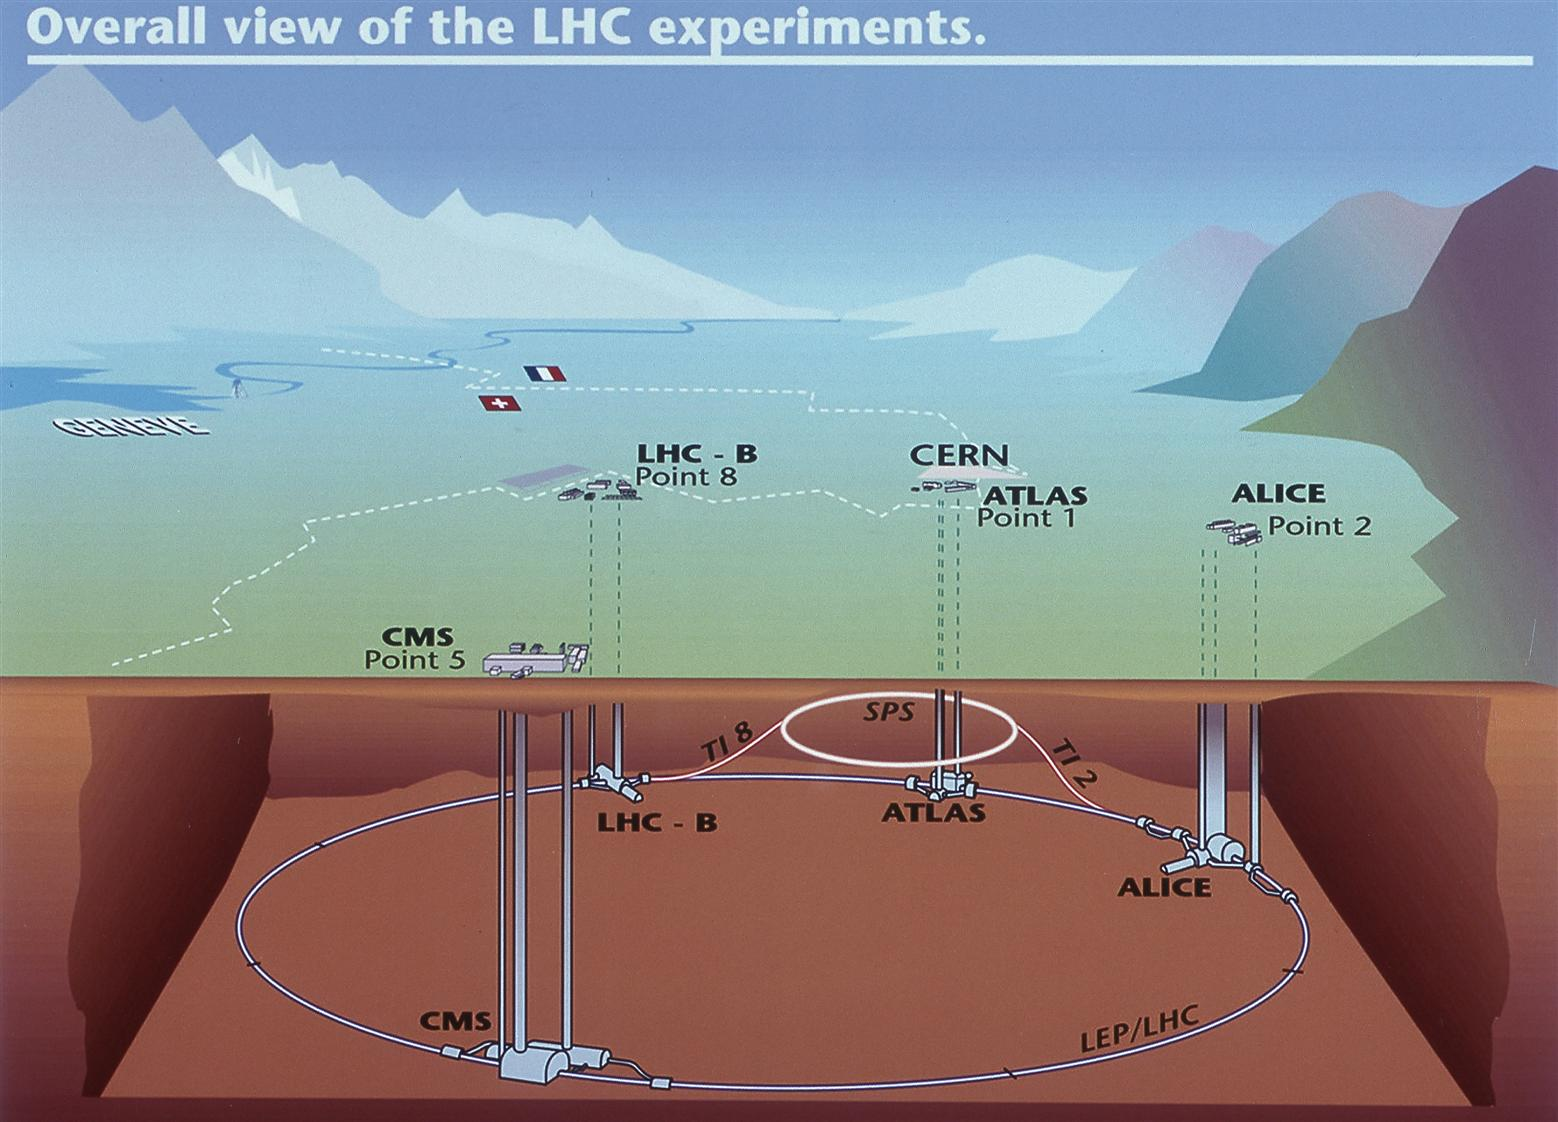
\includegraphics[width=5cm]{../img/lhc.jpg}
\end{backgroundblock}

\begin{itemize}
\item Large Hadron Collider (LHC)
	\begin{itemize}
	\item Particle accelerator
	\item $27~\kilo\meter$ circular tunnel
	\item 13 TeV
	\end{itemize}
\item High-Lumiosity LHC
	\begin{itemize}
	\item 10x beam lumiosity
	\item Increase in radiation \\ and amount of data
	\item $\rightarrow$ Gigabit Transceiver
	\end{itemize}
\end{itemize}

\end{frame}

%------------------------------------------------

\begin{frame}[t]
\frametitle{Gigabit Transceiver System}

\begin{backgroundblock}{7.5cm}{2.8cm}
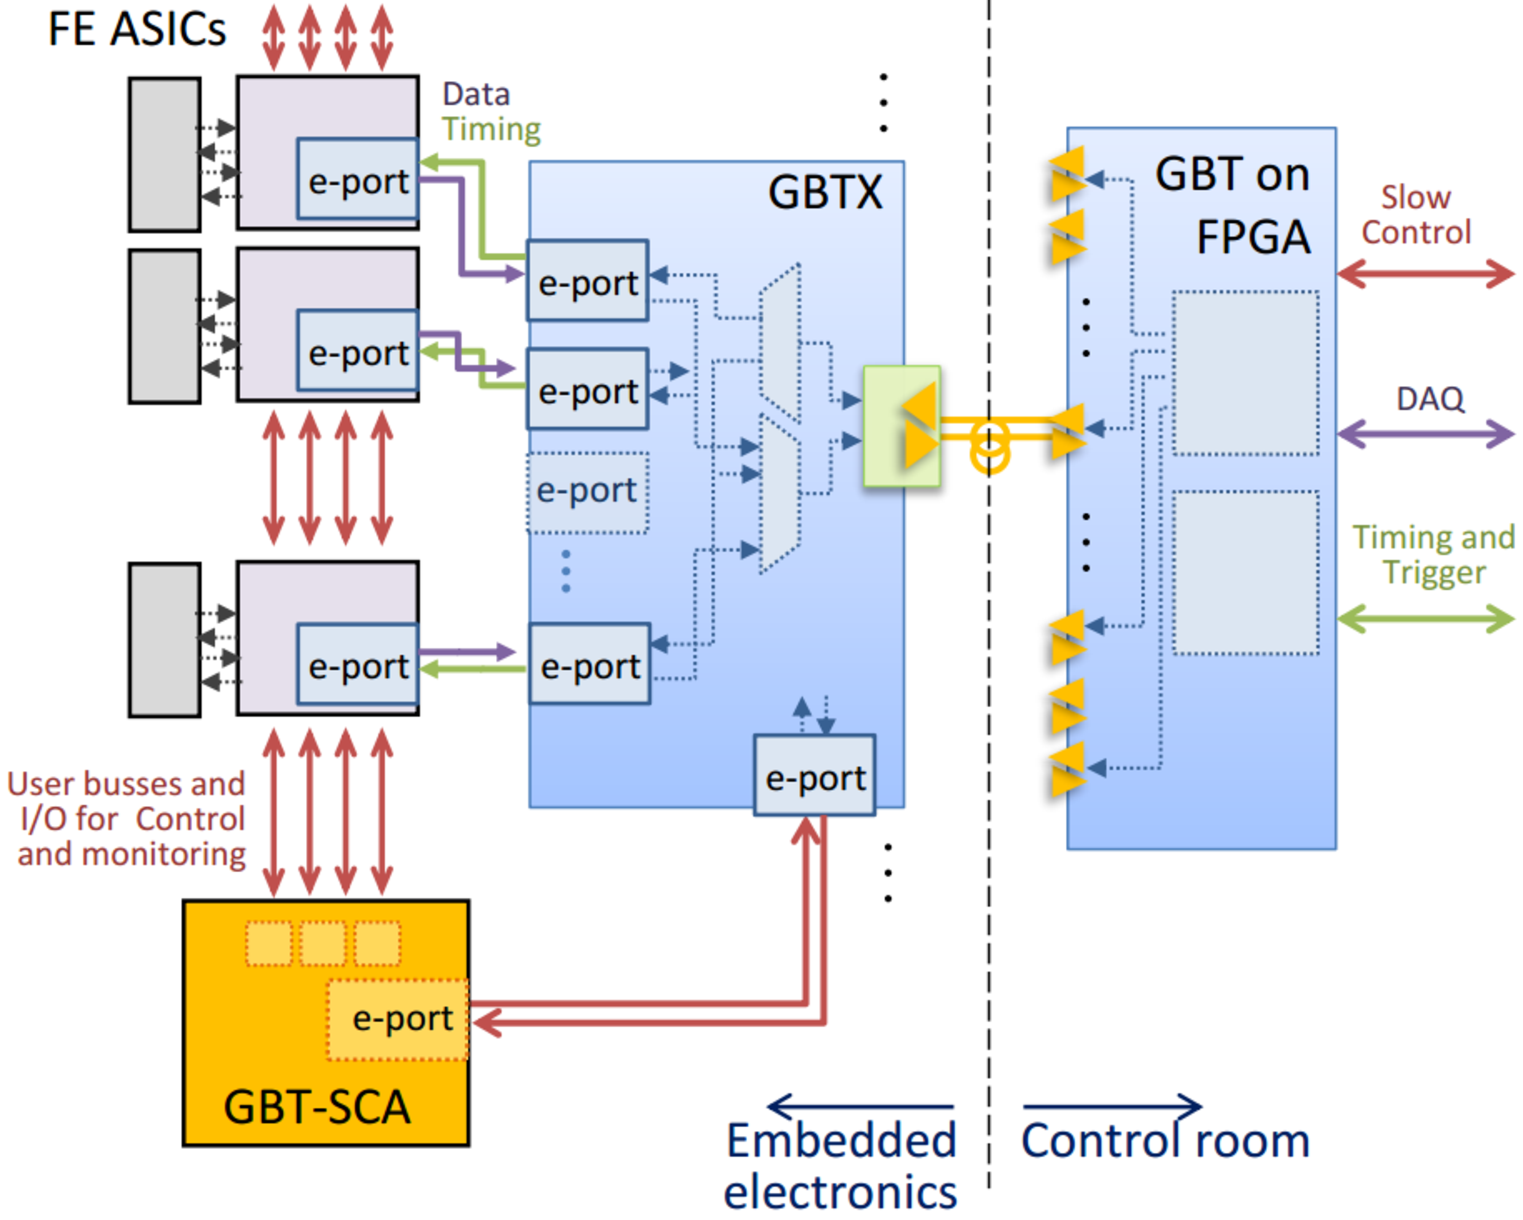
\includegraphics[width=5cm]{../img/gbtsys}
\end{backgroundblock}

\begin{itemize}
\item On-detector - Custom ASICs
	\begin{itemize}
	\item GBTx, GBT-SCA, VTTx/VTRx
	\item E-links
	\end{itemize}
\item Off-detector - Control room
	\begin{itemize}
	\item CRU (FPGA)
	\item \textgreater~ $4.8~\giga\bit\per\second$ transceivers
	\item GBT-FPGA
	\end{itemize}
\item Optical communication
	\begin{itemize}
	\item Timing and Trigger Control (TTC)
	\item Data Acquisition	(DAQ)
	\item Slow Control (SC)
	\end{itemize}
\end{itemize}

\begin{textblock*}{\paperwidth}(10pt,8cm)
{\small \color{gray} GBT - Gigabit Transceiver, CRU - Common Readout Unit \\ SCA - Slow Control Adapter, FPGA - Field-Programmable Gate Array}
\end{textblock*}

\end{frame}

%------------------------------------------------

\begin{frame}[t]
\frametitle{GBTx encoding modes}

\begin{backgroundblock}{1.5cm}{2.5cm}
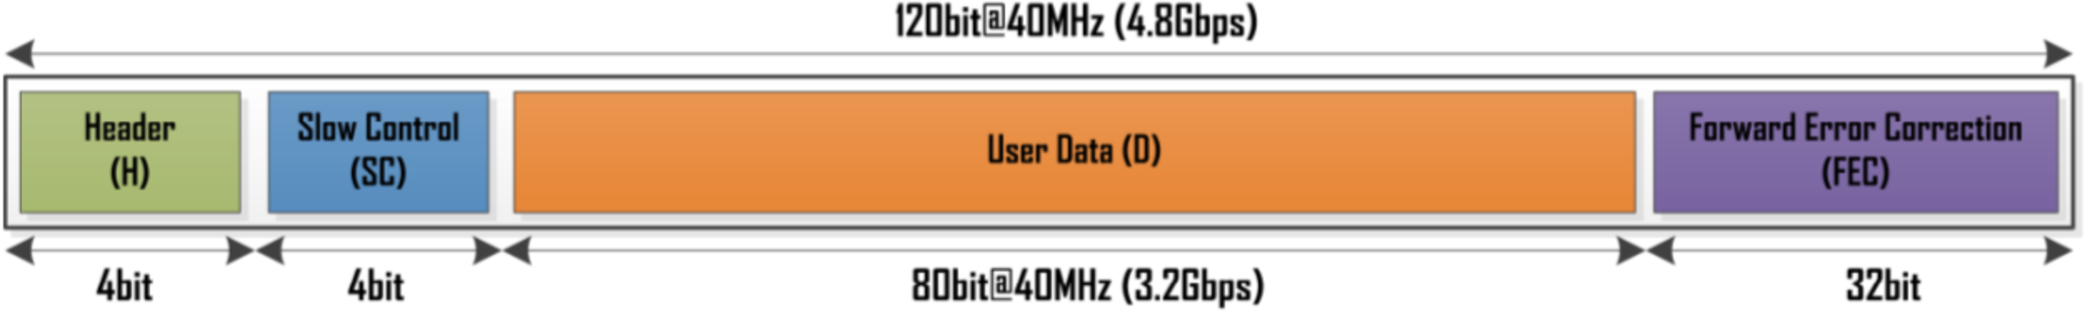
\includegraphics[width=10cm]{../img/gbtframe}
\end{backgroundblock}

\begin{backgroundblock}{1.5cm}{4.5cm}
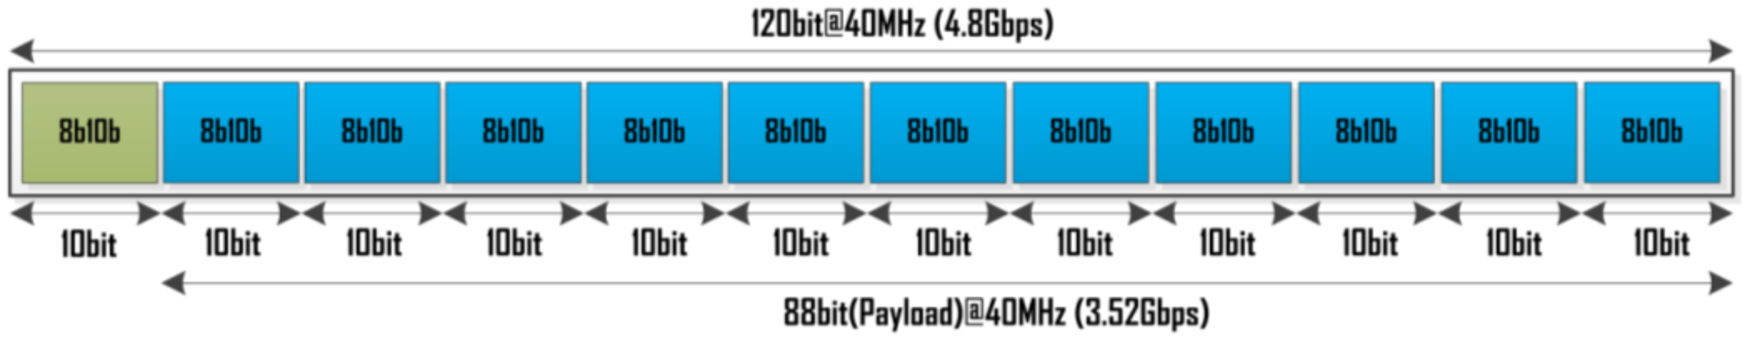
\includegraphics[width=10cm]{../img/8b10b}
\end{backgroundblock}

\begin{backgroundblock}{1.5cm}{6.7cm}
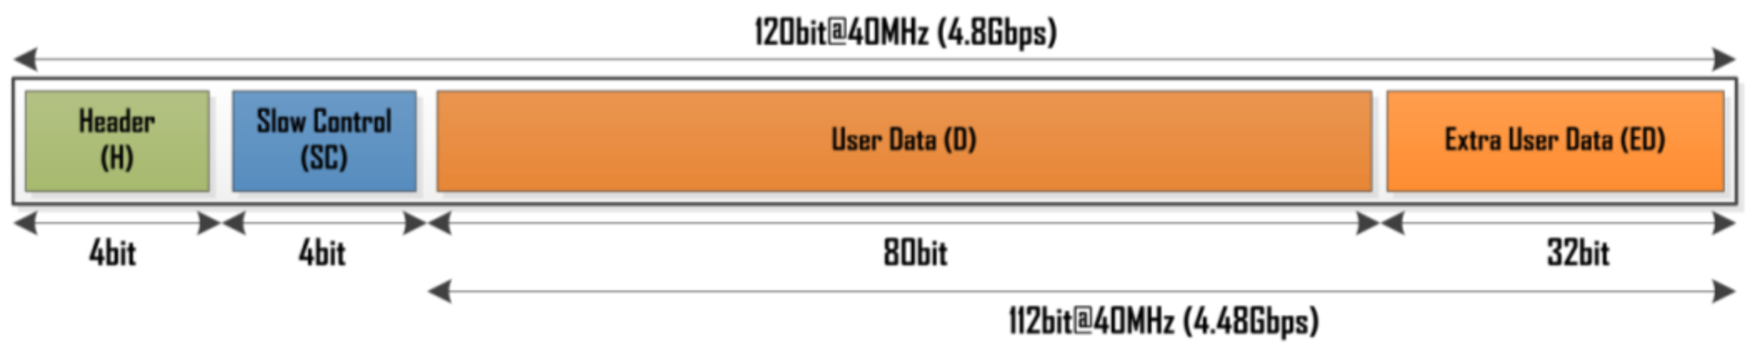
\includegraphics[width=10cm]{../img/widebus}
\end{backgroundblock}

\begin{itemize}
\item GBT-Frame - Standard \vspace{45pt}
\item 8B/10B  \vspace{45pt}
\item Wide-Bus  \vspace{45pt}
\end{itemize}

\begin{textblock*}{\paperwidth}(4cm,9cm)
{\tiny \color{gray} (figures taken from the GBT-FPGA User Manual)}
\end{textblock*}

\end{frame}

%------------------------------------------------

\begin{frame}
\frametitle{GBT-FPGA}

%\begin{figure}
\begin{backgroundblock}{7.5cm}{2.8cm}
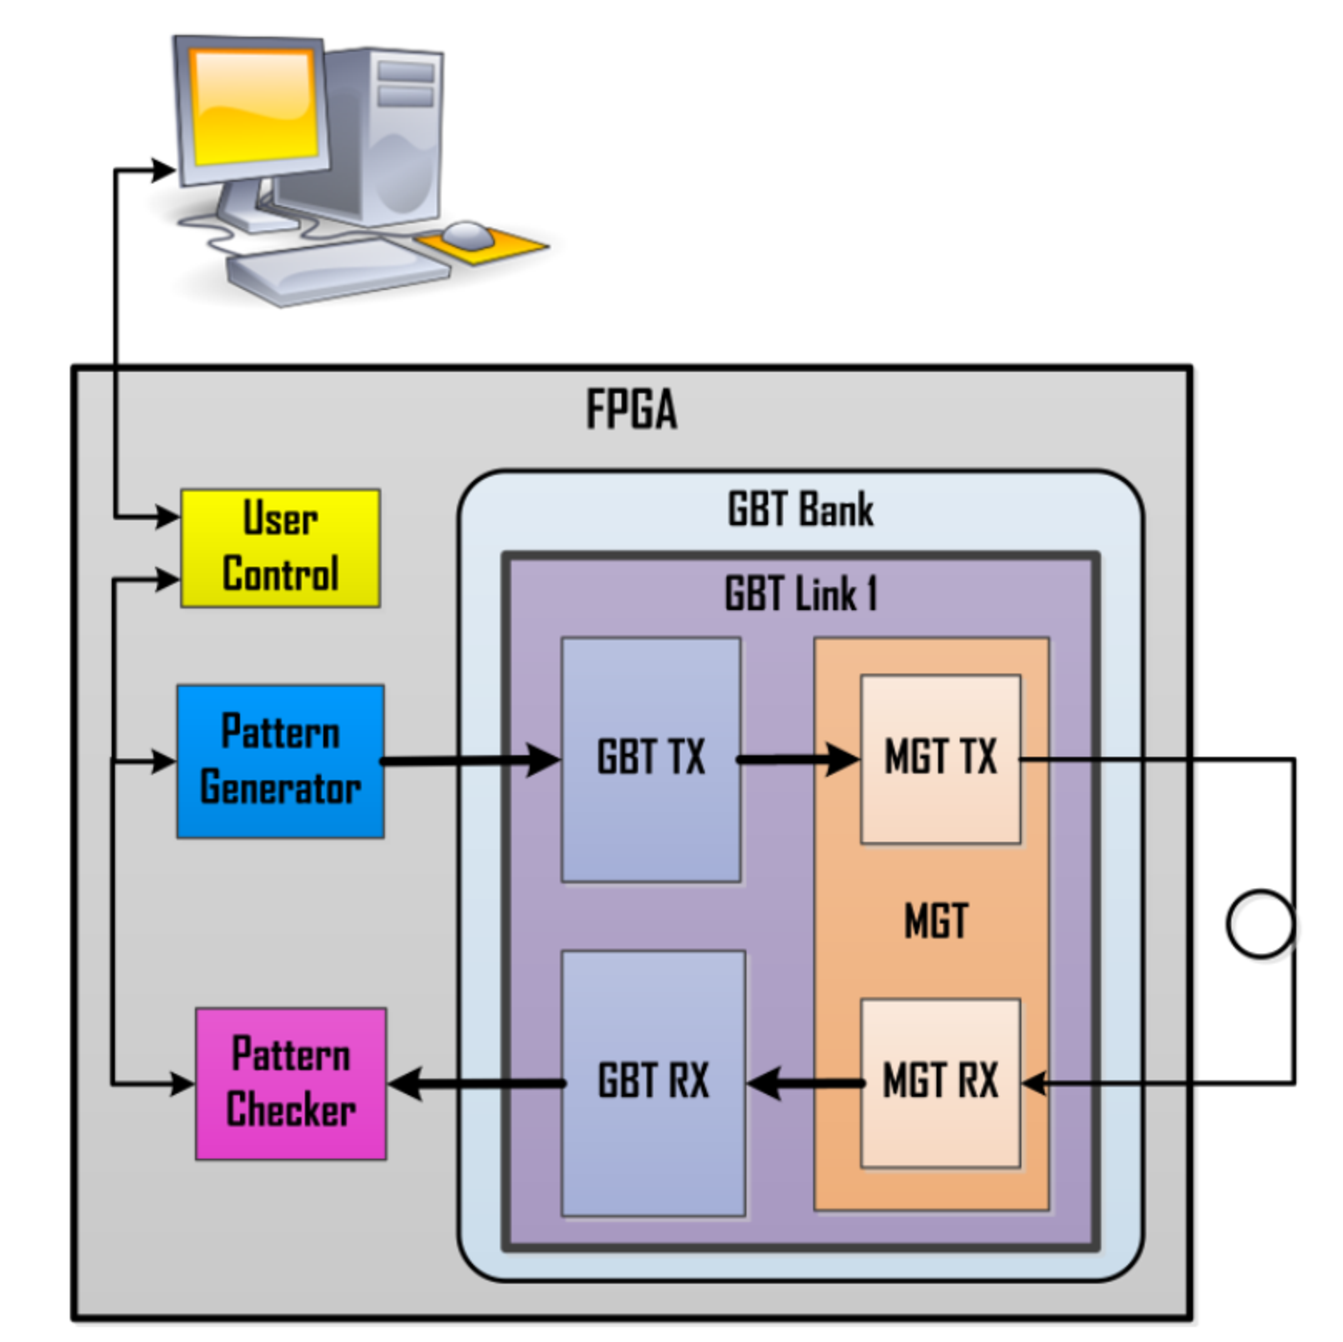
\includegraphics[width=5cm]{../img/gbtex}
\end{backgroundblock}
%\caption{GBT example design \cite{gbt_fpga}}
%\end{figure}

\begin{itemize}
\item Firmware library for \\ Altera/Xilinx FPGAs
\item GBT Link
	\begin{itemize}
	\item "Standard", "Latency-Optimized"
	\item GBT Rx, GBT Tx, GBT MGT 
	\end{itemize}
\item GBT-example Design
\end{itemize}

\begin{textblock*}{\paperwidth}(10pt,8cm)
{\small \color{gray} MGT - Multi-Gigabit Transceiver}
\end{textblock*}

\end{frame}

%------------------------------------------------

\begin{frame}
\frametitle{Versatile Link Demo Board (VLDB)}
%\begin{figure}
\begin{backgroundblock}{2.5cm}{2.5cm}
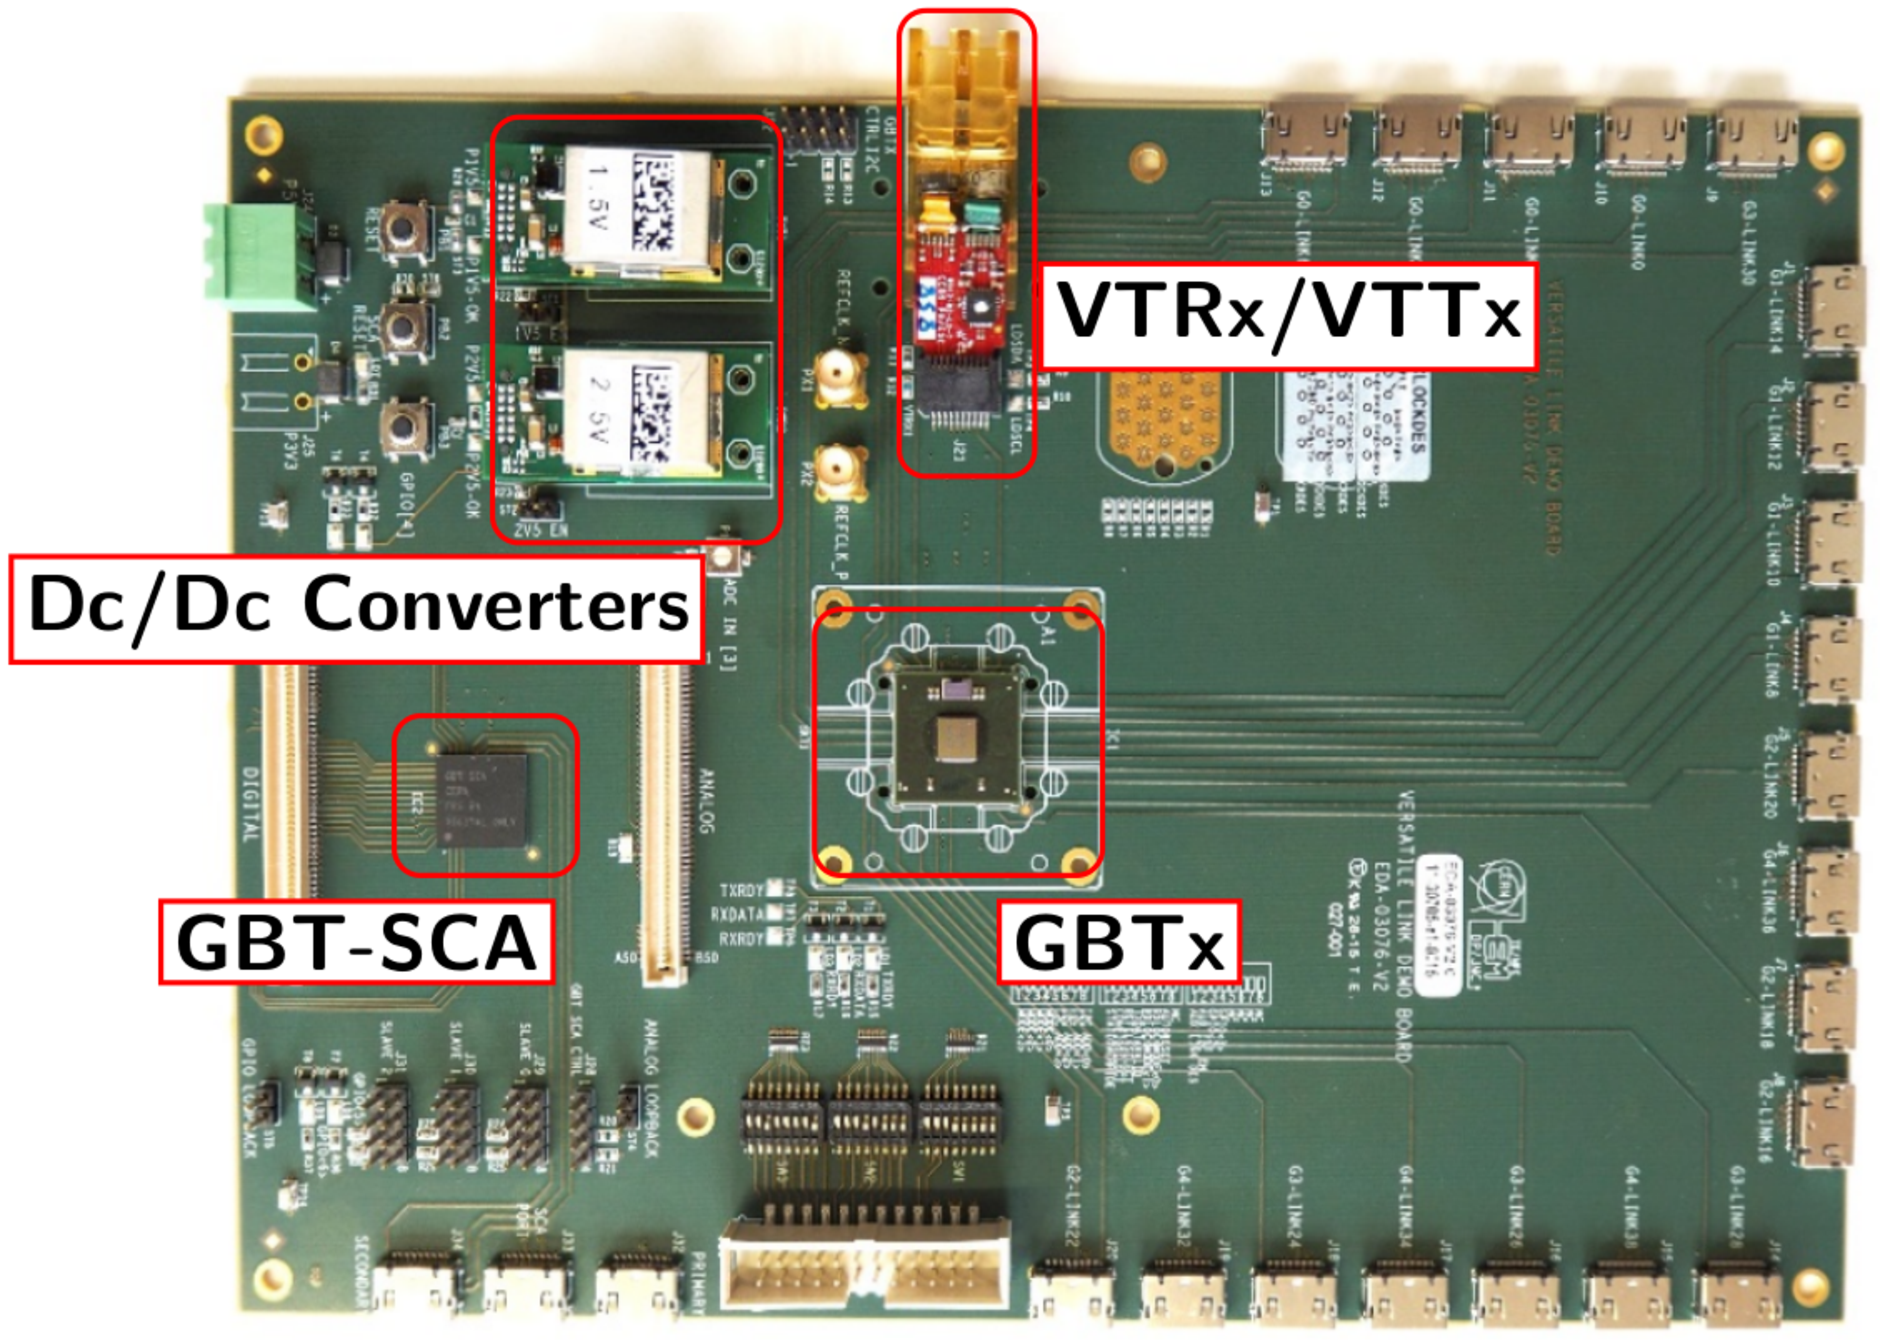
\includegraphics[width=0.6\paperwidth]{../img/vldbex}
\end{backgroundblock}
%\caption{GBT example design \cite{gbt_fpga}}
%\end{figure}
\end{frame}


%------------------------------------------------

\begin{frame}
\frametitle{Primary Objective}

\begin{itemize}
\item Software Design
	\begin{itemize}
	\item Serial communication between PC and CRU
	\item Interface allowing control over CRU
	\end{itemize}
\item PCB Design
	\begin{itemize}
	\item Connection between CRU and VLDB 
	\item HDMI for e-link communication
	\item High-speed Optical-Fiber module for GBT-frame
	\end{itemize}
\end{itemize}

\begin{textblock*}{\paperwidth}(10pt,8cm)
{\small \color{gray} CRU - Common Readout Unit \\ VLDB - Versatile Link Demo Board}
\end{textblock*}

\end{frame}

%------------------------------------------------

%------------------------------------------------
\section{PCB Design}
%------------------------------------------------
\subsection{Design Discussion} 
\subsection{Transmission Lines} 
\subsection{Design Parameters}
%------------------------------------------------

\begin{frame}
\frametitle{PCB Design}

\begin{backgroundblock}{1.8cm}{2.0cm}
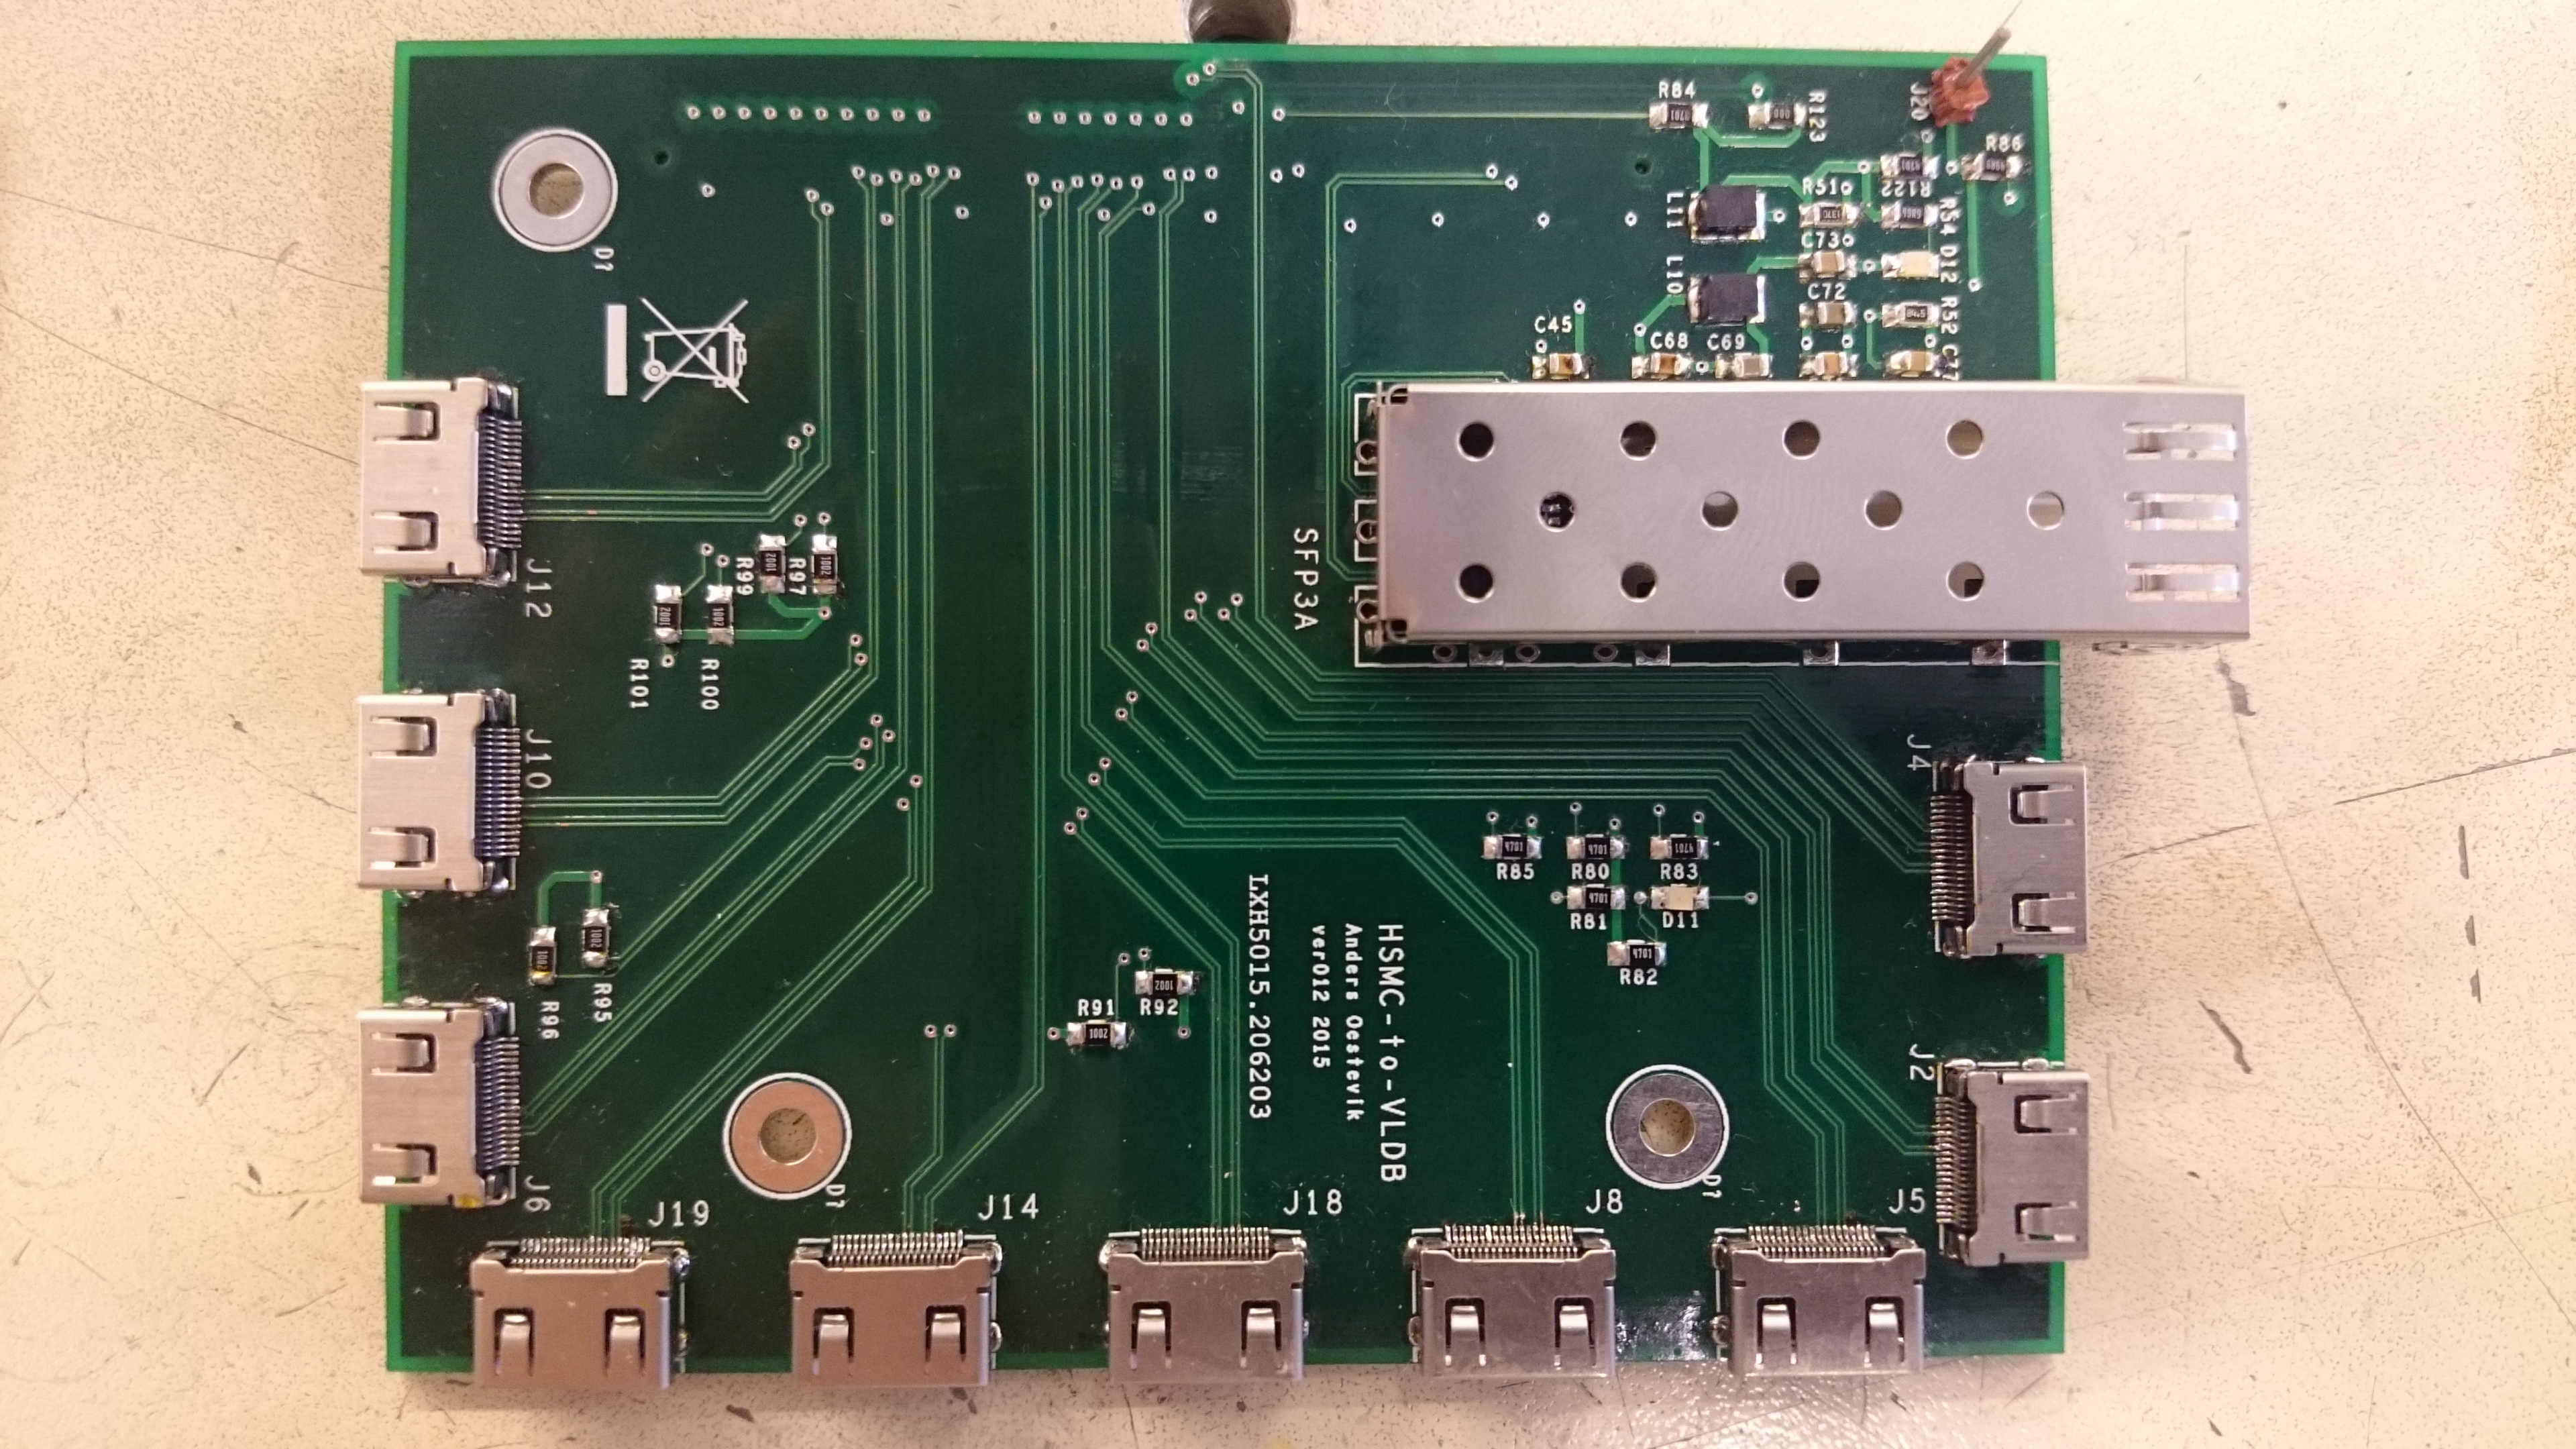
\includegraphics[width=0.7\paperwidth, trim={16cm 0cm 15cm 0cm}, clip]{../img/pcb_1.JPG}
\end{backgroundblock}

\end{frame}
%------------------------------------------------

\begin{frame}
\frametitle{PCB Design}

\begin{backgroundblock}{6.2cm}{2.0cm}
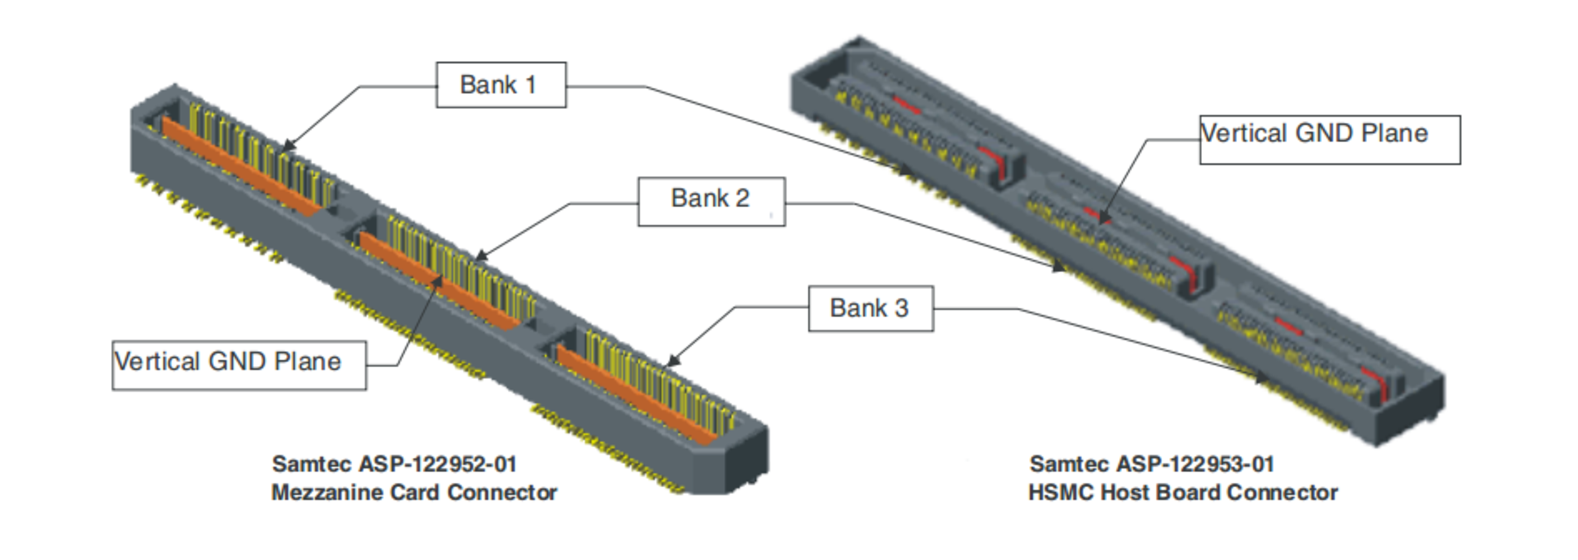
\includegraphics[width=0.5\paperwidth]{../img/HSMC_52_53_hsmcspec.pdf}
\end{backgroundblock}
\Large Specifications:\\
\normalsize
\begin{itemize}
\item Connect board between CRU and VLDB using HSMC-connector
\item E-links $\rightarrow$ $320~\mega\bit\per\second$ detector data $\rightarrow$ LVDS
\item Optical-Fiber $\rightarrow$ $4.8~\giga\bit\per\second$ GBT data $\rightarrow$ PCML
\end{itemize}

\begin{textblock*}{\paperwidth}(10pt,8cm)
{\small \color{gray} HSMC - High-Speed Mezzanine Card \\ LVDS - Low-Voltage Differential Signaling \\ PCML - Pseudo Current Mode Logic}
\end{textblock*}

\end{frame}
%------------------------------------------------

\begin{frame}
\frametitle{PCB Design}

\begin{backgroundblock}{3.7cm}{2.0cm}
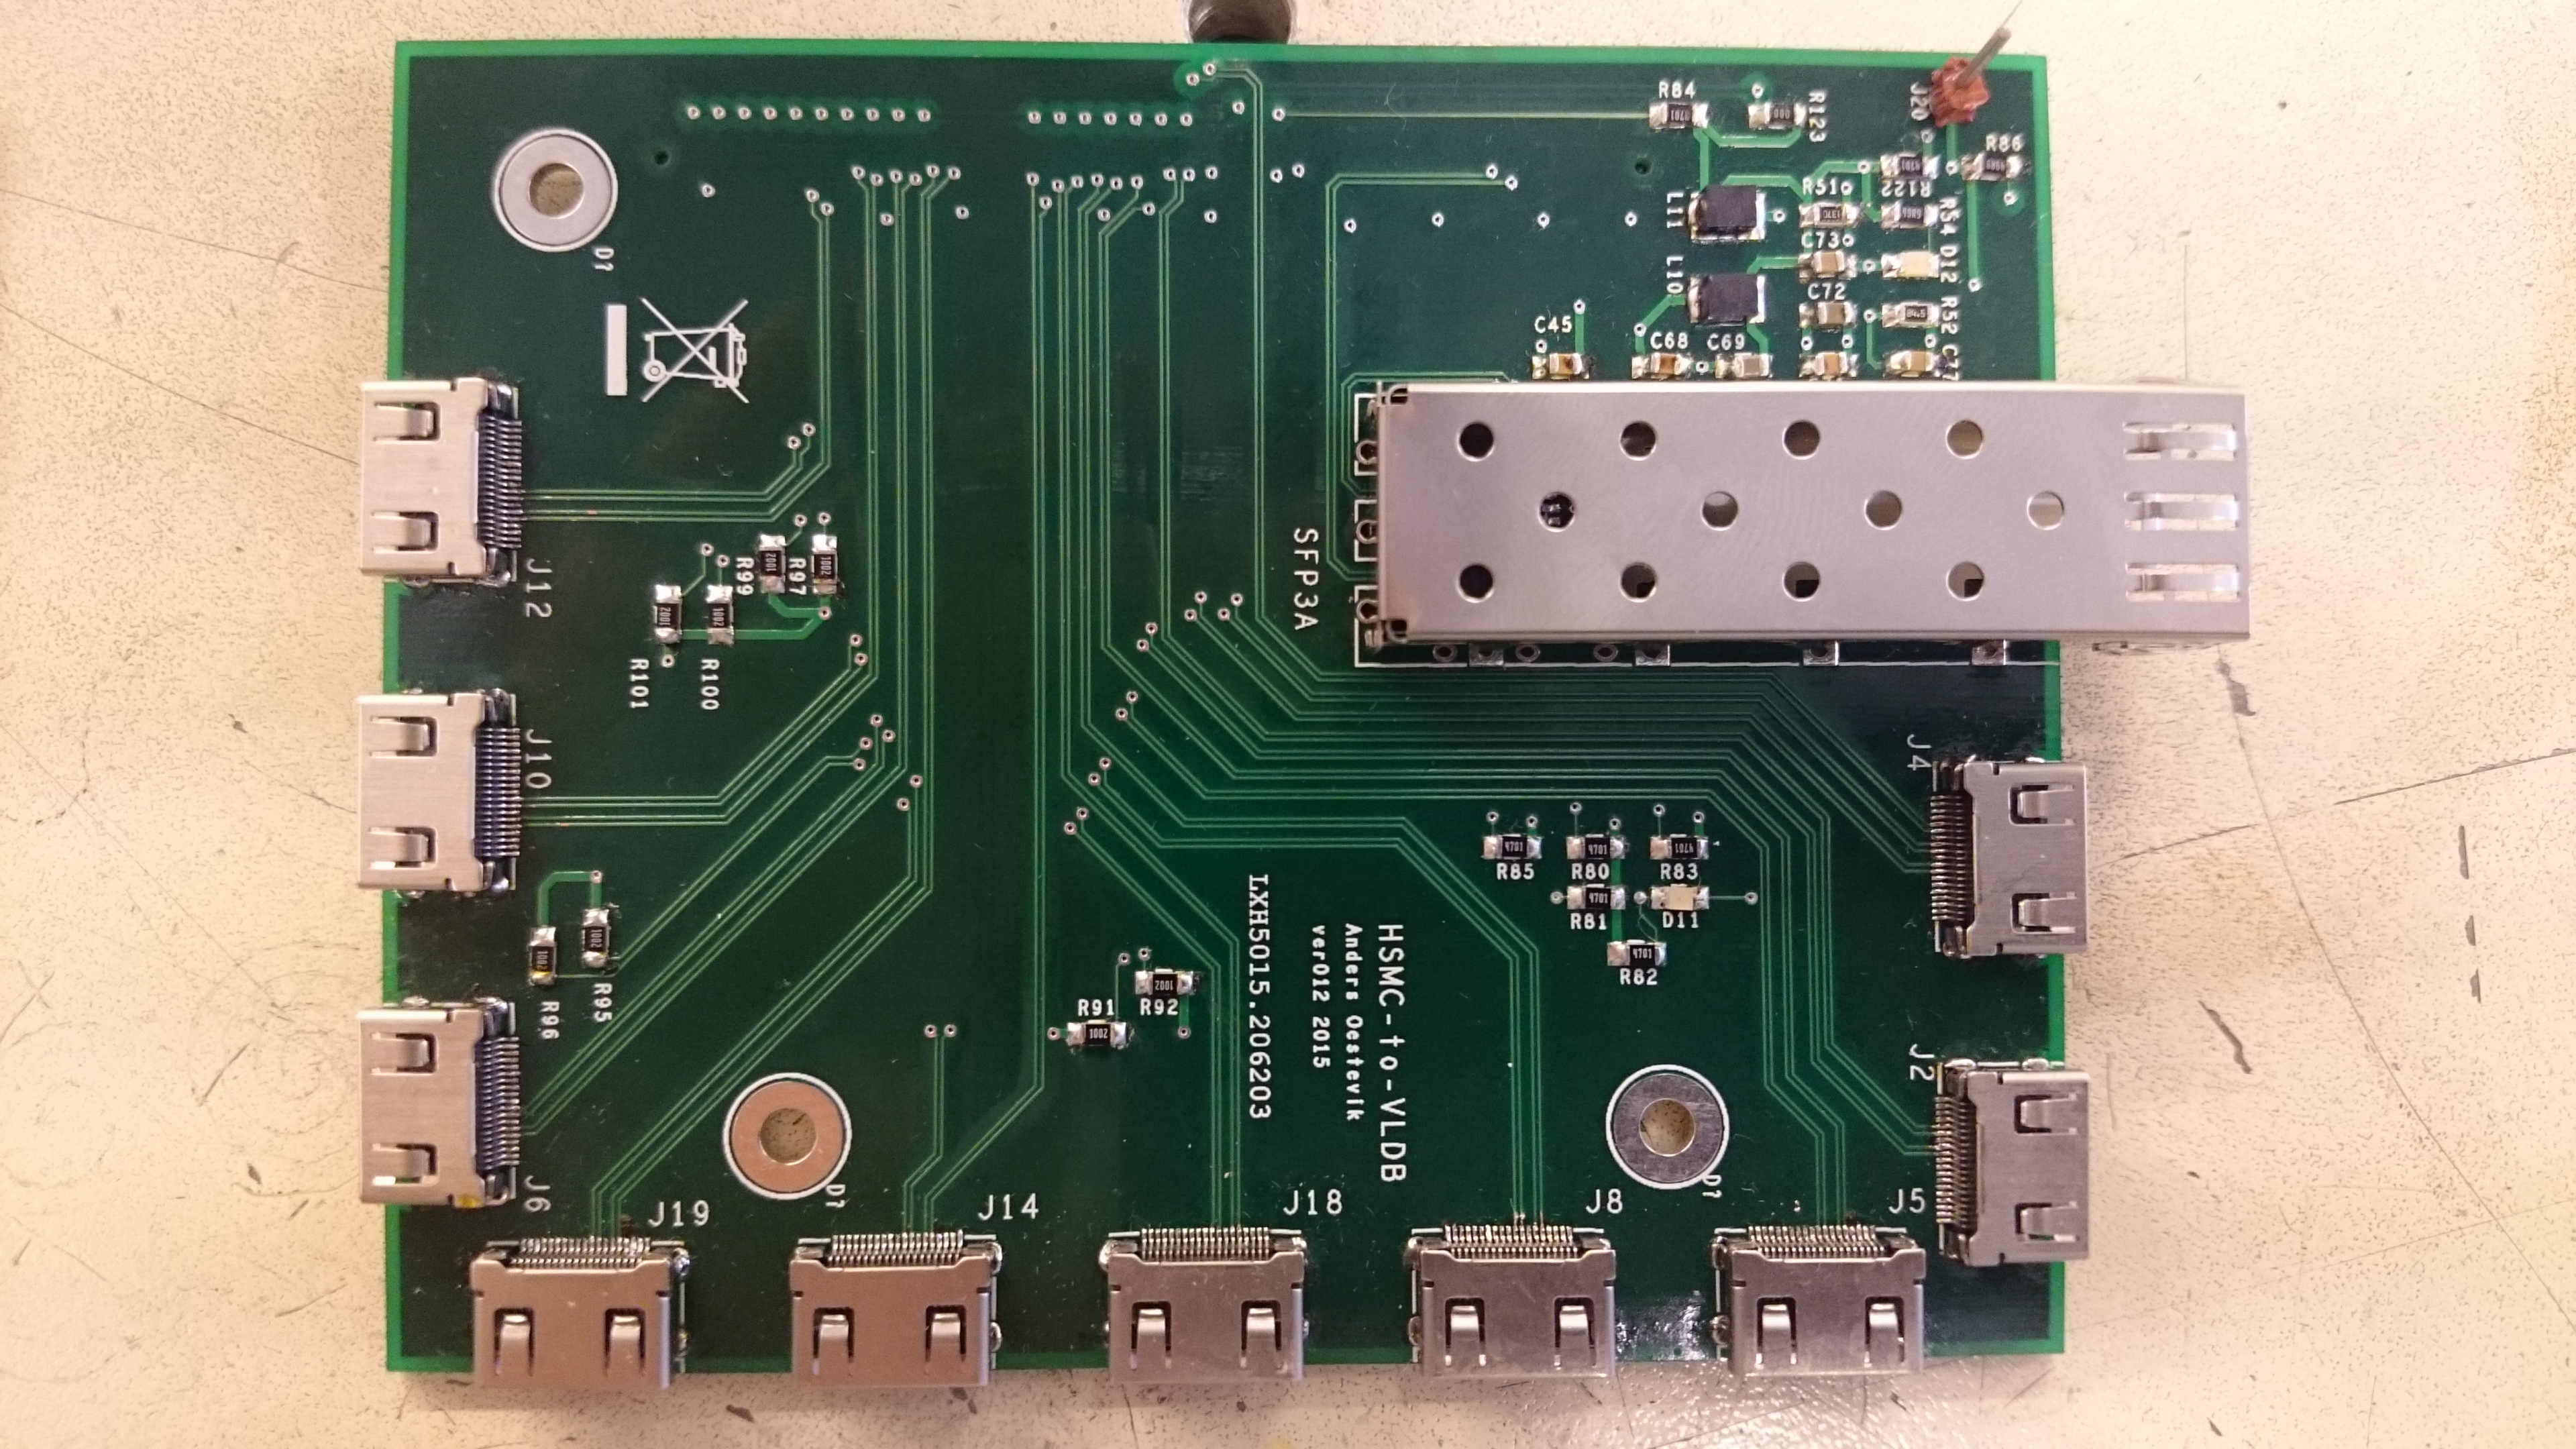
\includegraphics[width=0.2\paperwidth, trim={16cm 0cm 15cm 0cm}, clip]{../img/pcb_1.JPG}
\end{backgroundblock}

\begin{textblock*}{\paperwidth}(4.5cm,4.2cm)
{\color{black} \Huge \textbf{$\uparrow$}}
\end{textblock*}

\begin{backgroundblock}{9cm}{2.0cm}
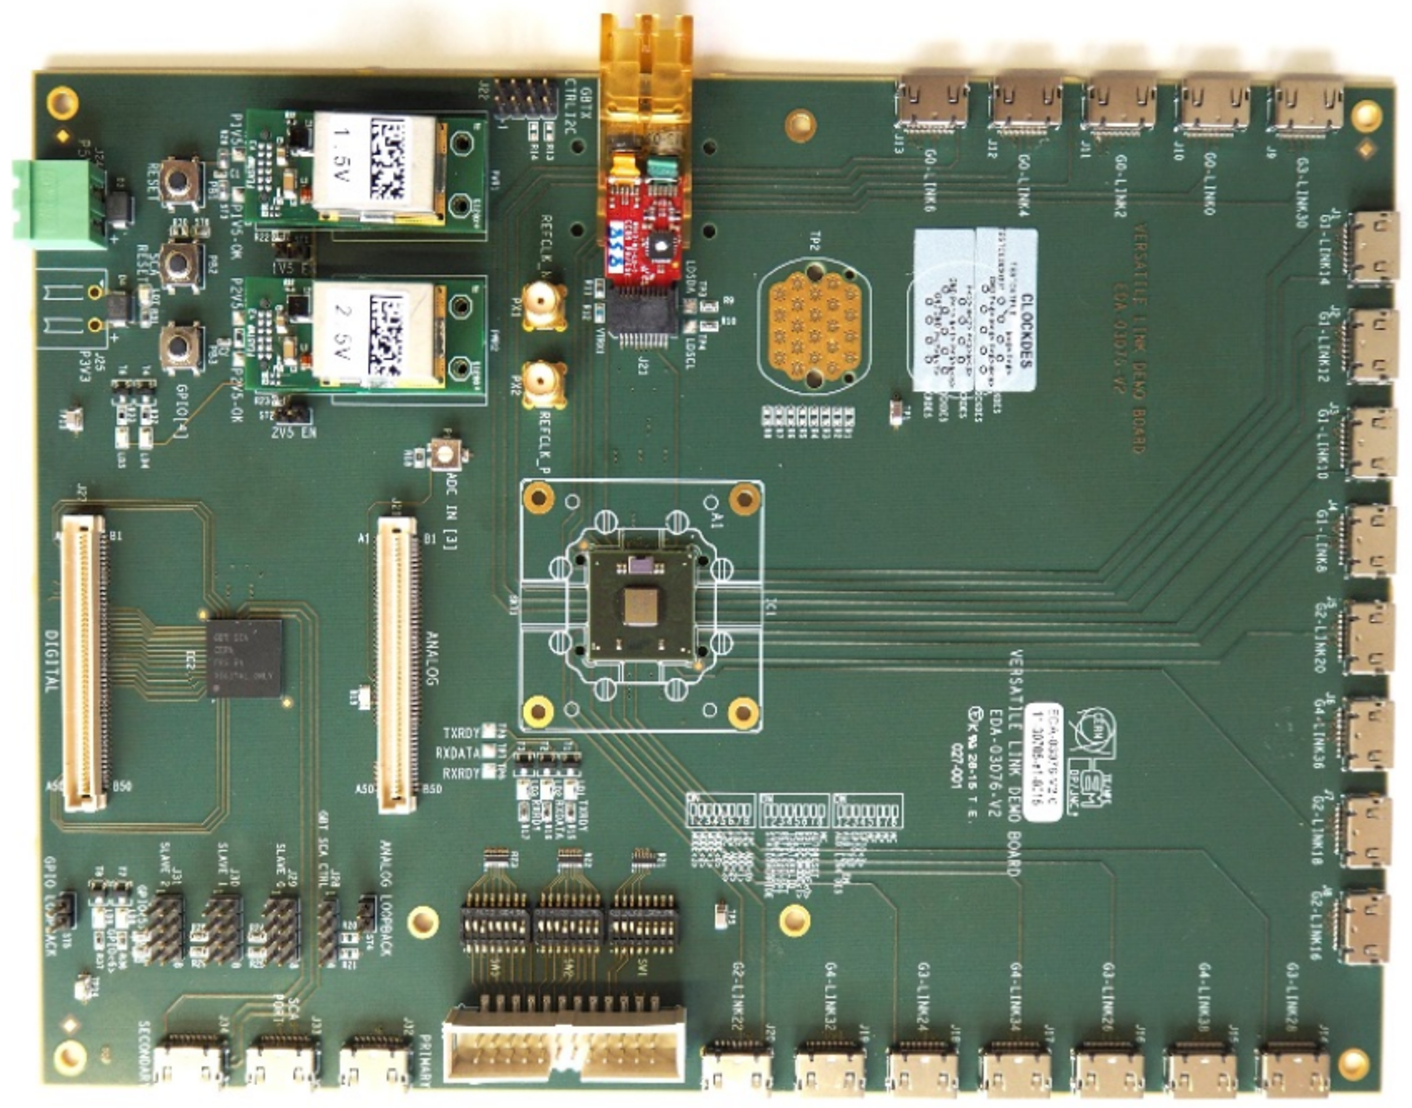
\includegraphics[width=0.2\paperwidth]{../img/vldb.pdf}
\end{backgroundblock}

\begin{textblock*}{\paperwidth}(10.0cm,4.2cm)
{\color{black} \Huge \textbf{$\uparrow$}}
\end{textblock*}

\begin{backgroundblock}{1.3cm}{5cm}
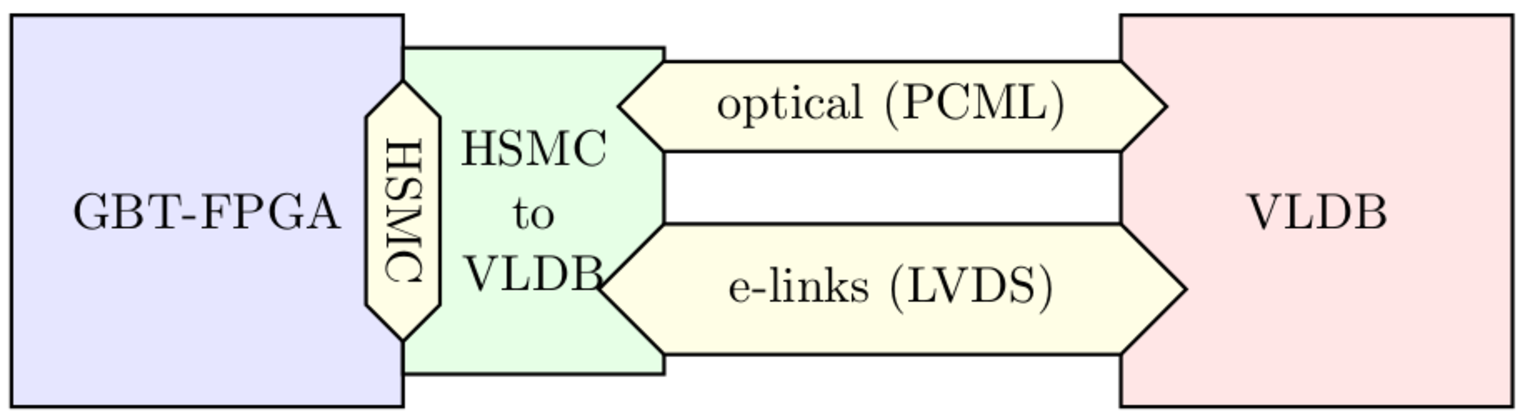
\includegraphics[width=0.8\paperwidth]{../img/pcbdia.pdf}
\end{backgroundblock}
\end{frame}
%------------------------------------------------

\begin{frame}[t]
\frametitle{PCB Design}
\begin{backgroundblock}{0.5cm}{4cm}
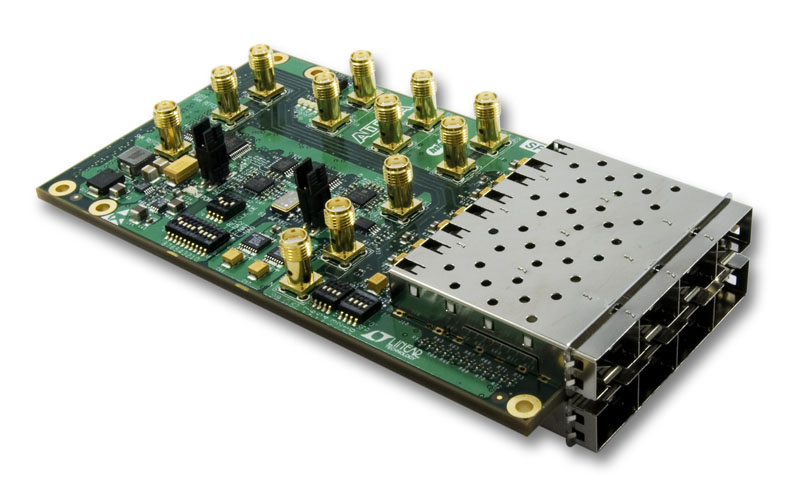
\includegraphics[width=0.4\paperwidth]{../img/sfp.jpg}
\end{backgroundblock}

\begin{textblock*}{\paperwidth}(6cm,5.5cm)
{\color{black} \Huge \textbf{$\rightarrow$}}
\end{textblock*}

\begin{backgroundblock}{7.5cm}{4.0cm}
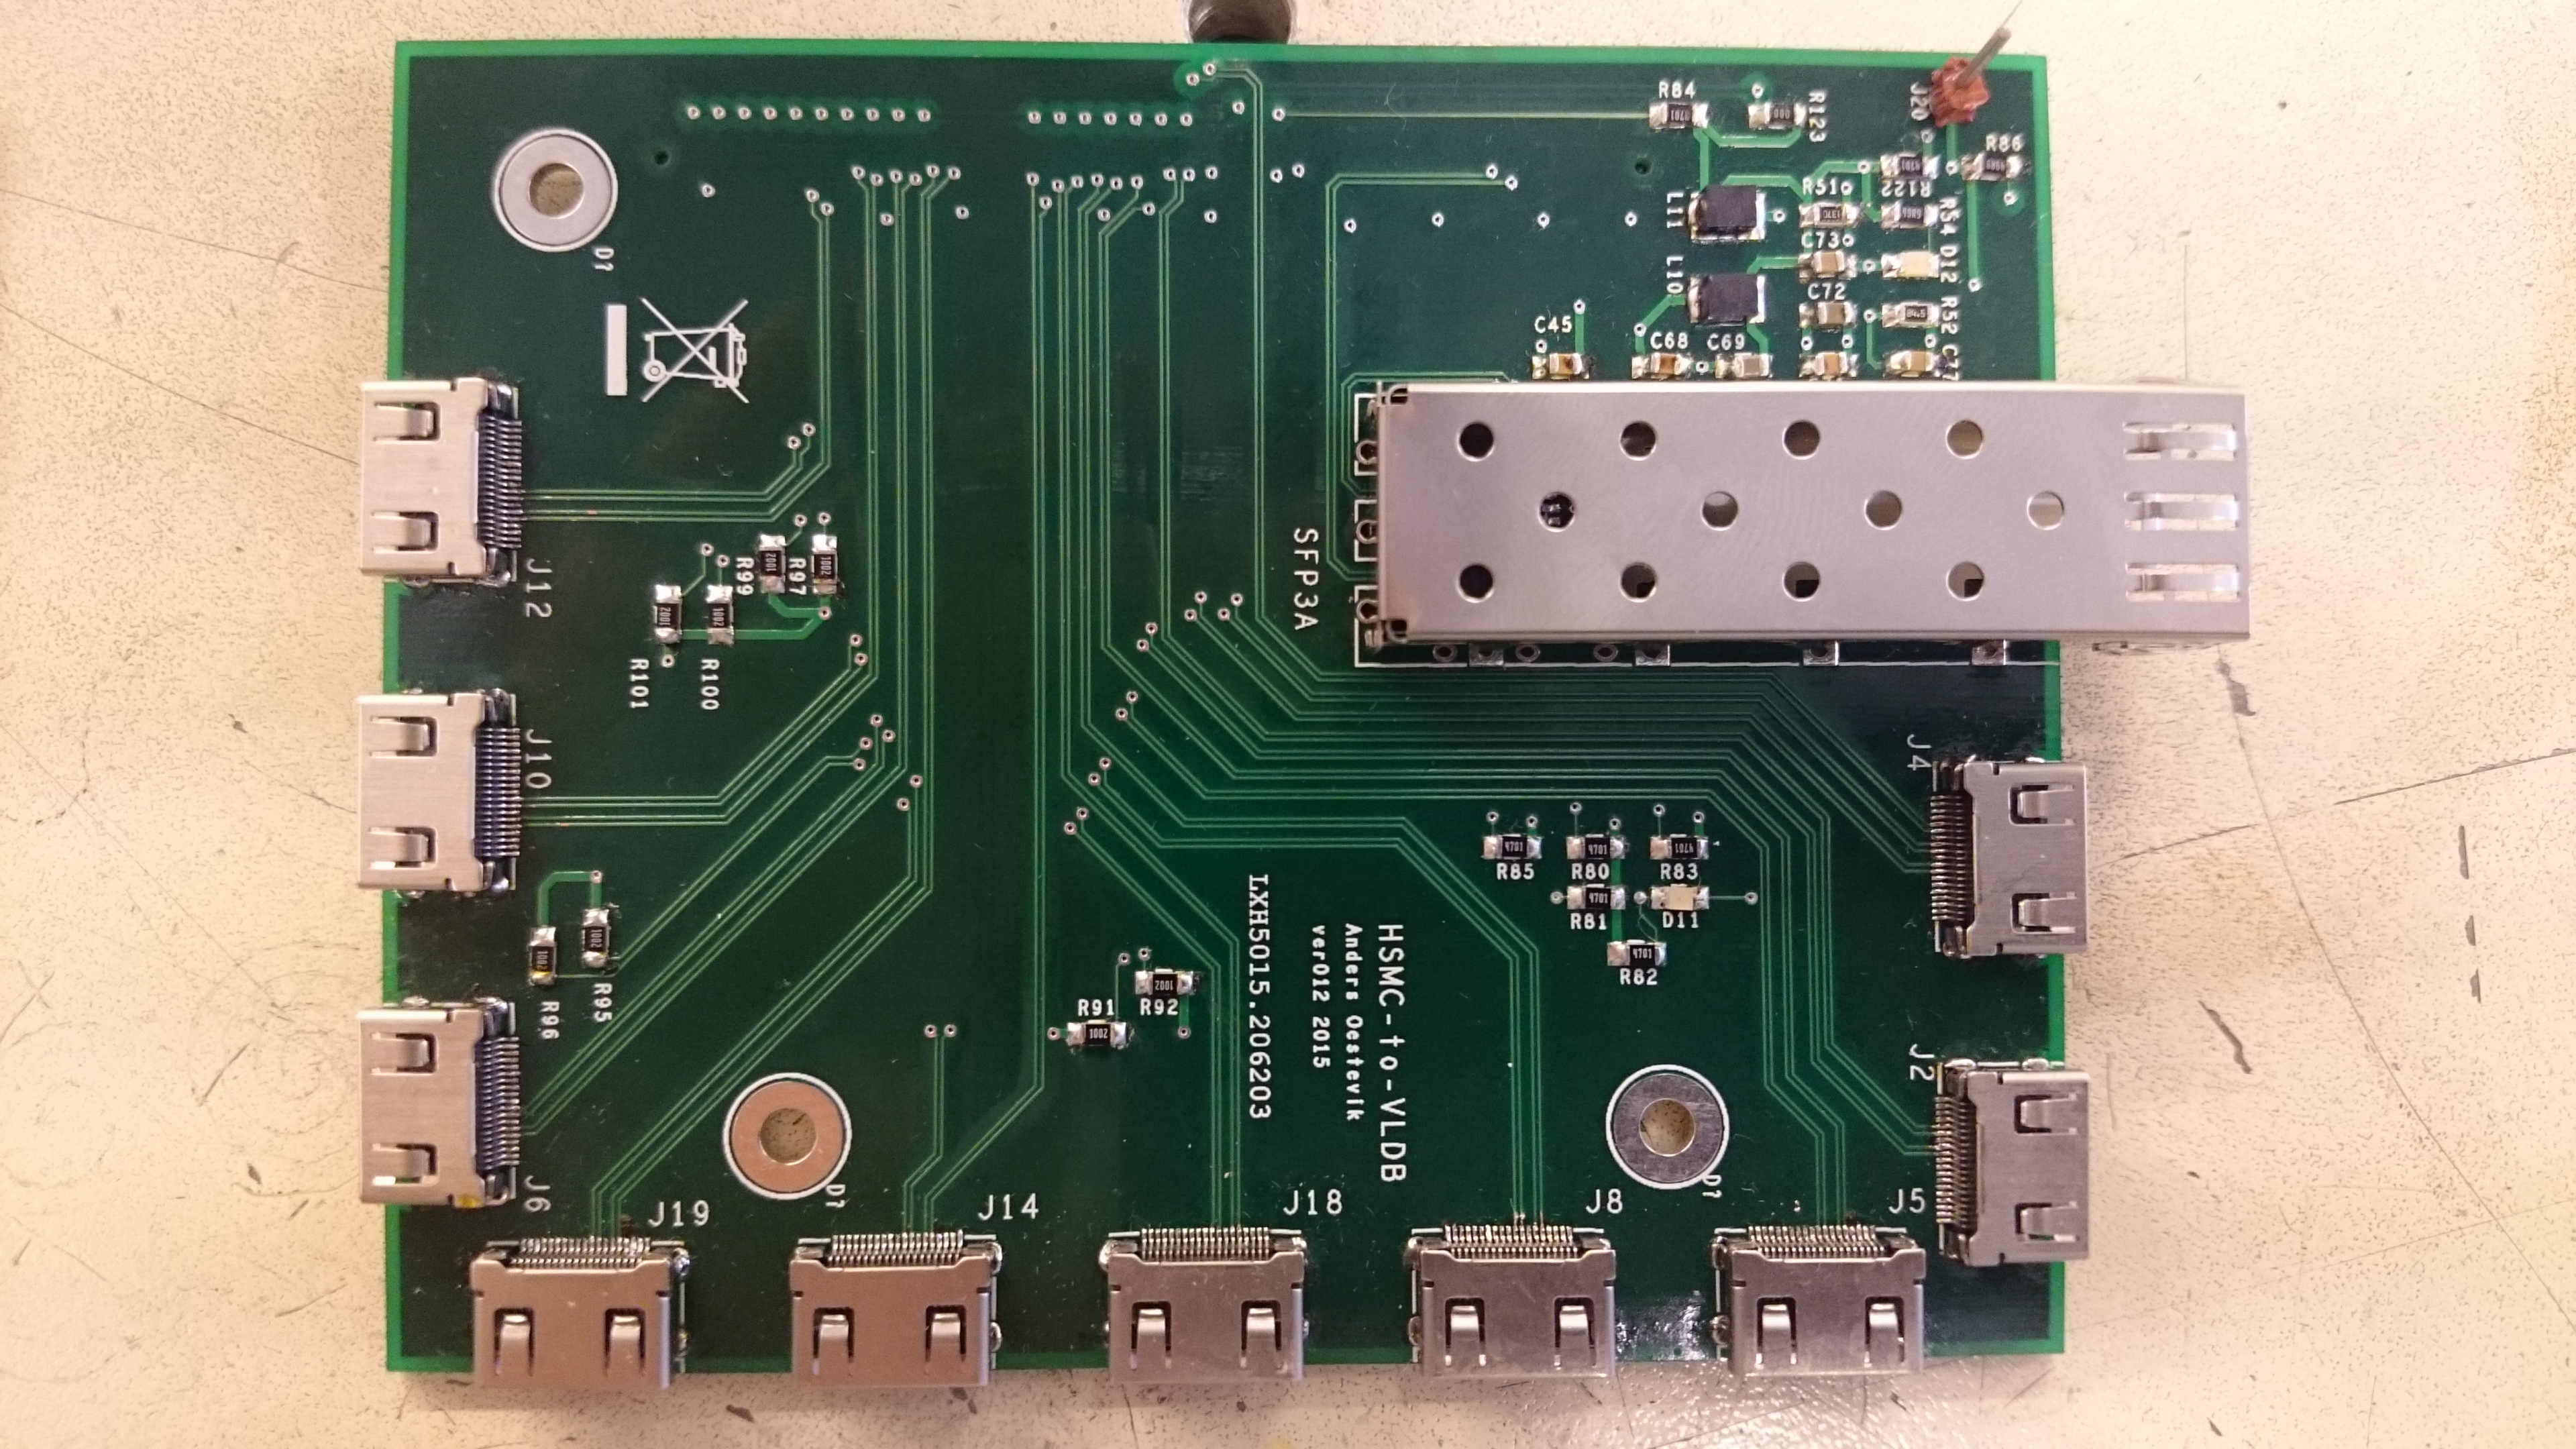
\includegraphics[width=0.35\paperwidth, trim={16cm 0cm 15cm 0cm}, clip]{../img/pcb_1.JPG}
\end{backgroundblock}

\begin{textblock*}{\paperwidth}(0.5cm,7cm)
{\tiny \color{gray} (\url{http://www.terasic.com.tw/} \\ \url{attachment/archive/342/image/SFP_003_800.jpg})}
\end{textblock*}

\begin{textblock*}{\paperwidth}(1cm,3.8cm)
{\color{black} SFP HSMC board}
\end{textblock*}

\begin{textblock*}{\paperwidth}(10pt,8cm)
{\small \color{gray} SFP - Small Form-Factor Pluggable \\ HSMC - High-Speed Mezzanine Card}
\end{textblock*}

\begin{itemize}
\item Each HDMI has an input pair and an output pair
\item J4 has an additional pair for input clock from VLDB
\end{itemize}

\end{frame}
%------------------------------------------------

\begin{frame}[t]
\frametitle{Transmission Lines}

\begin{backgroundblock}{7.5cm}{7.0cm}
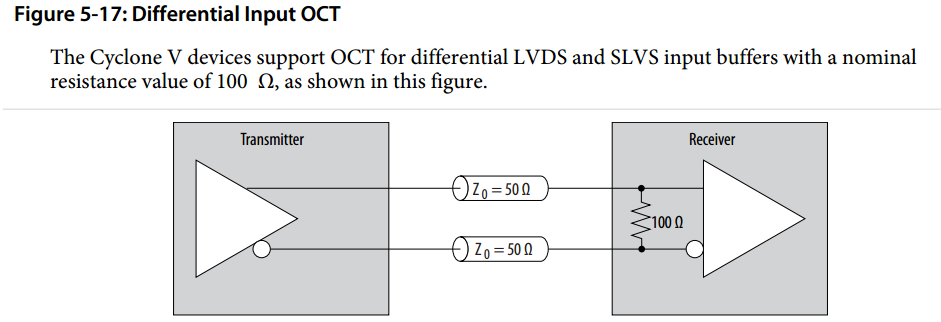
\includegraphics[width=0.4\paperwidth]{../img/altera_z0.png}
\end{backgroundblock}

\begin{align*}
 	v = \frac{c}{\sqrt{\epsilon_r}},~
 	\epsilon_r \approx 4
 \end{align*}

\begin{itemize}
\item $v = 15~\centi\meter\per\nano\second$
\item $4.8~\giga\bit\per\second~(0.2~\nano\second)$ $\rightarrow$ \\ transmission line if trace \textless~ $3.1~\centi\meter$
\item Characteristic impedance, $Z_0 = 50$
\item Differential impedance, $Z_{diff} = 100$
\end{itemize}

\end{frame}
%------------------------------------------------

\begin{frame}[t]
\frametitle{Transmission Lines}

\begin{backgroundblock}{2.0cm}{6cm}
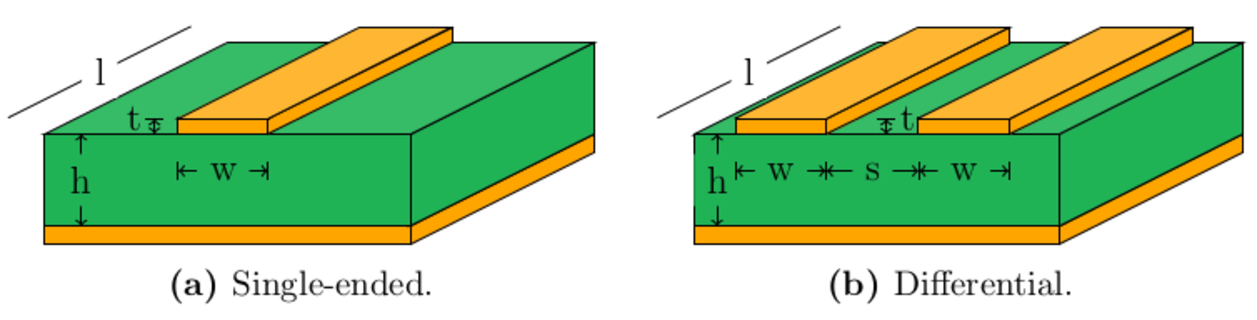
\includegraphics[width=0.7\paperwidth]{../img/umstrip.pdf}
\end{backgroundblock}

\begin{align*}
    Z_0 = \frac{60}{\sqrt{0.475\epsilon_r + 0.67}} \times \ln{\frac{4h}{0.67(0.8w + t)}}
 \end{align*}

 \begin{align*}
    Z_{diff} = 2 \times Z_0 [1 - 0.48 e^{(-0.96 \times \frac{s}{h})}]
\end{align*}

\end{frame}
%------------------------------------------------

\begin{frame}[t]
\frametitle{Design Parameters}

\begin{backgroundblock}{1.2cm}{4.5cm}
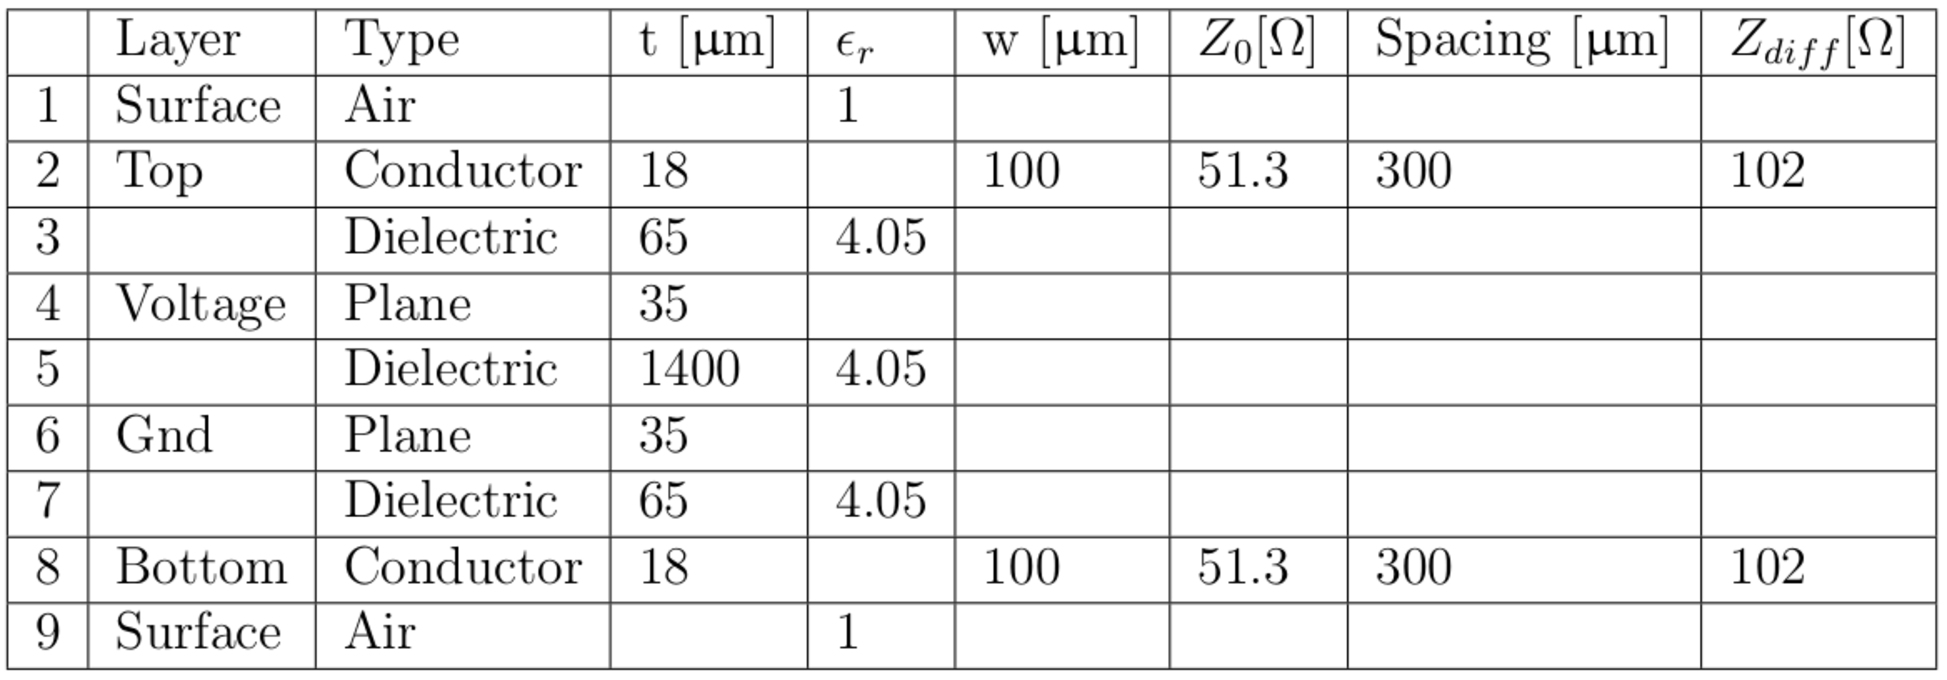
\includegraphics[width=0.8\paperwidth]{../img/designpar.pdf}
\end{backgroundblock}

\begin{itemize}
\item Routing differential signals:
	\begin{itemize}
	\item Equal trace lengths on each pair
	\item As close as possible, but keep distance to other pairs
	\item As straight paths as possible
	\end{itemize}
\end{itemize}

\end{frame}
%------------------------------------------------

\begin{frame}[t]
\frametitle{Result}

\begin{backgroundblock}{4.0cm}{2.0cm}
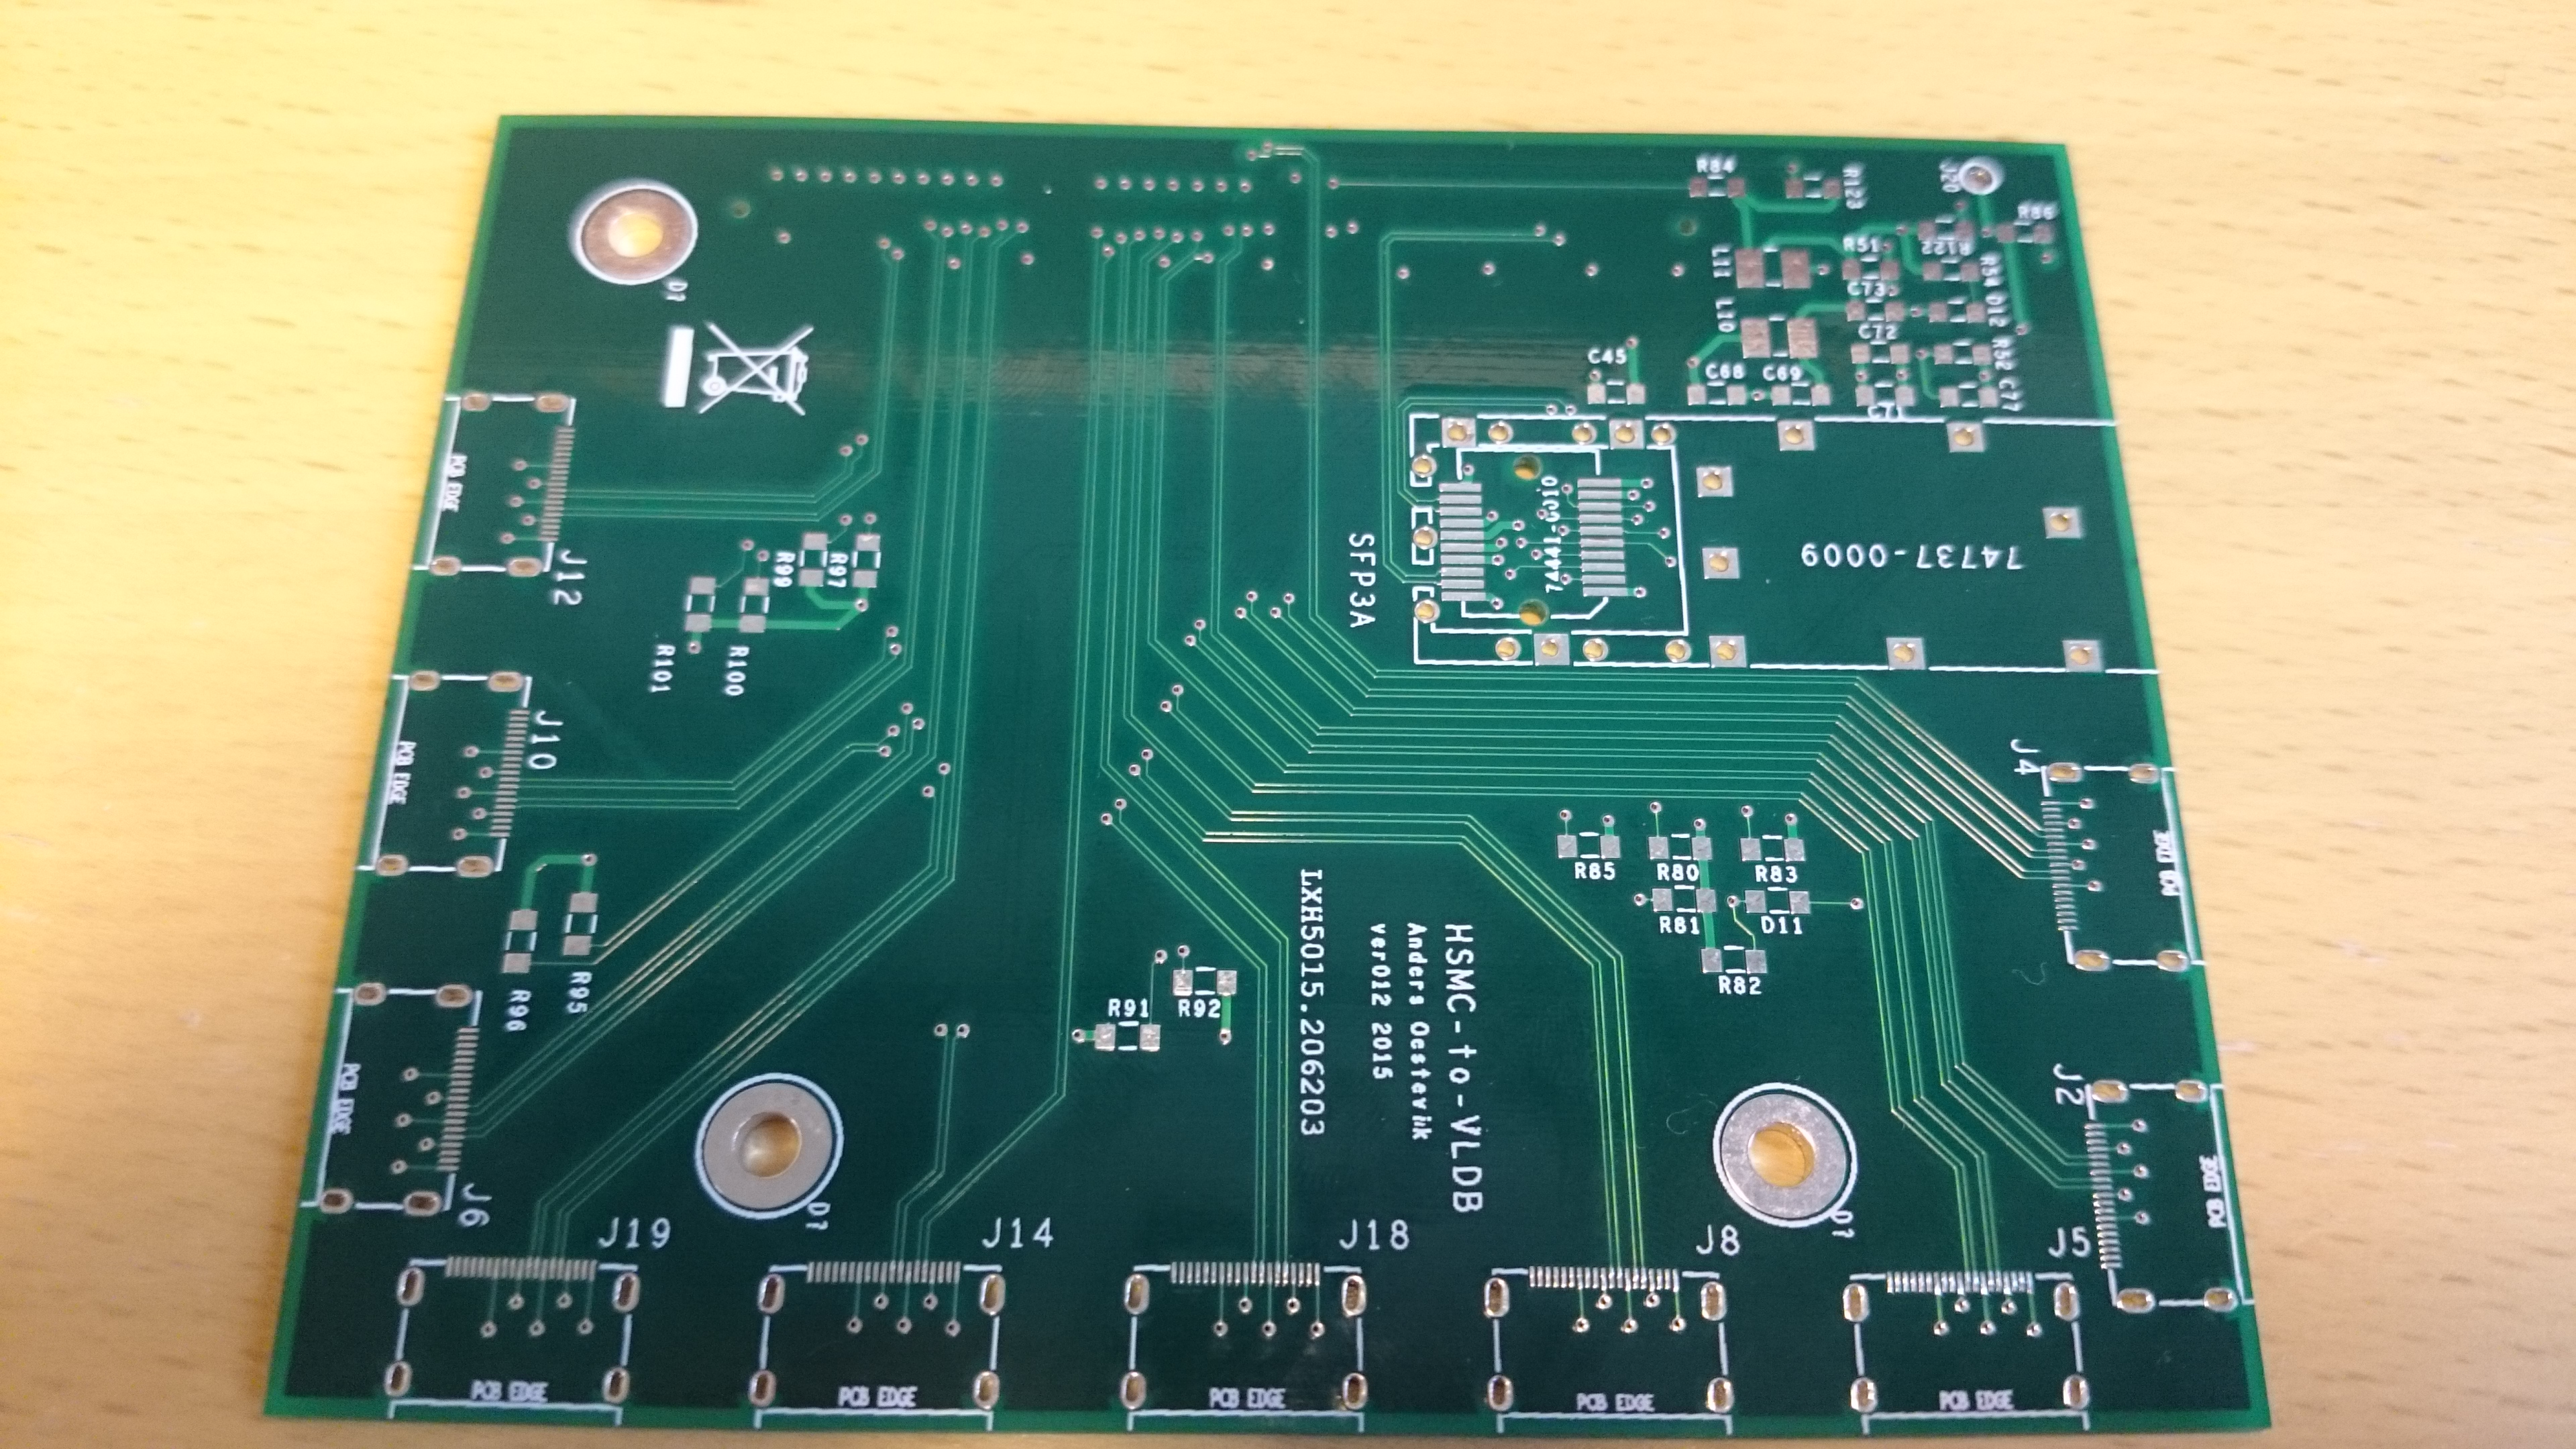
\includegraphics[width=0.4\paperwidth, trim={14cm 0cm 15cm 5cm}, clip]{../img/pcbbare.JPG}
\end{backgroundblock}

\begin{backgroundblock}{7.0cm}{6.0cm}
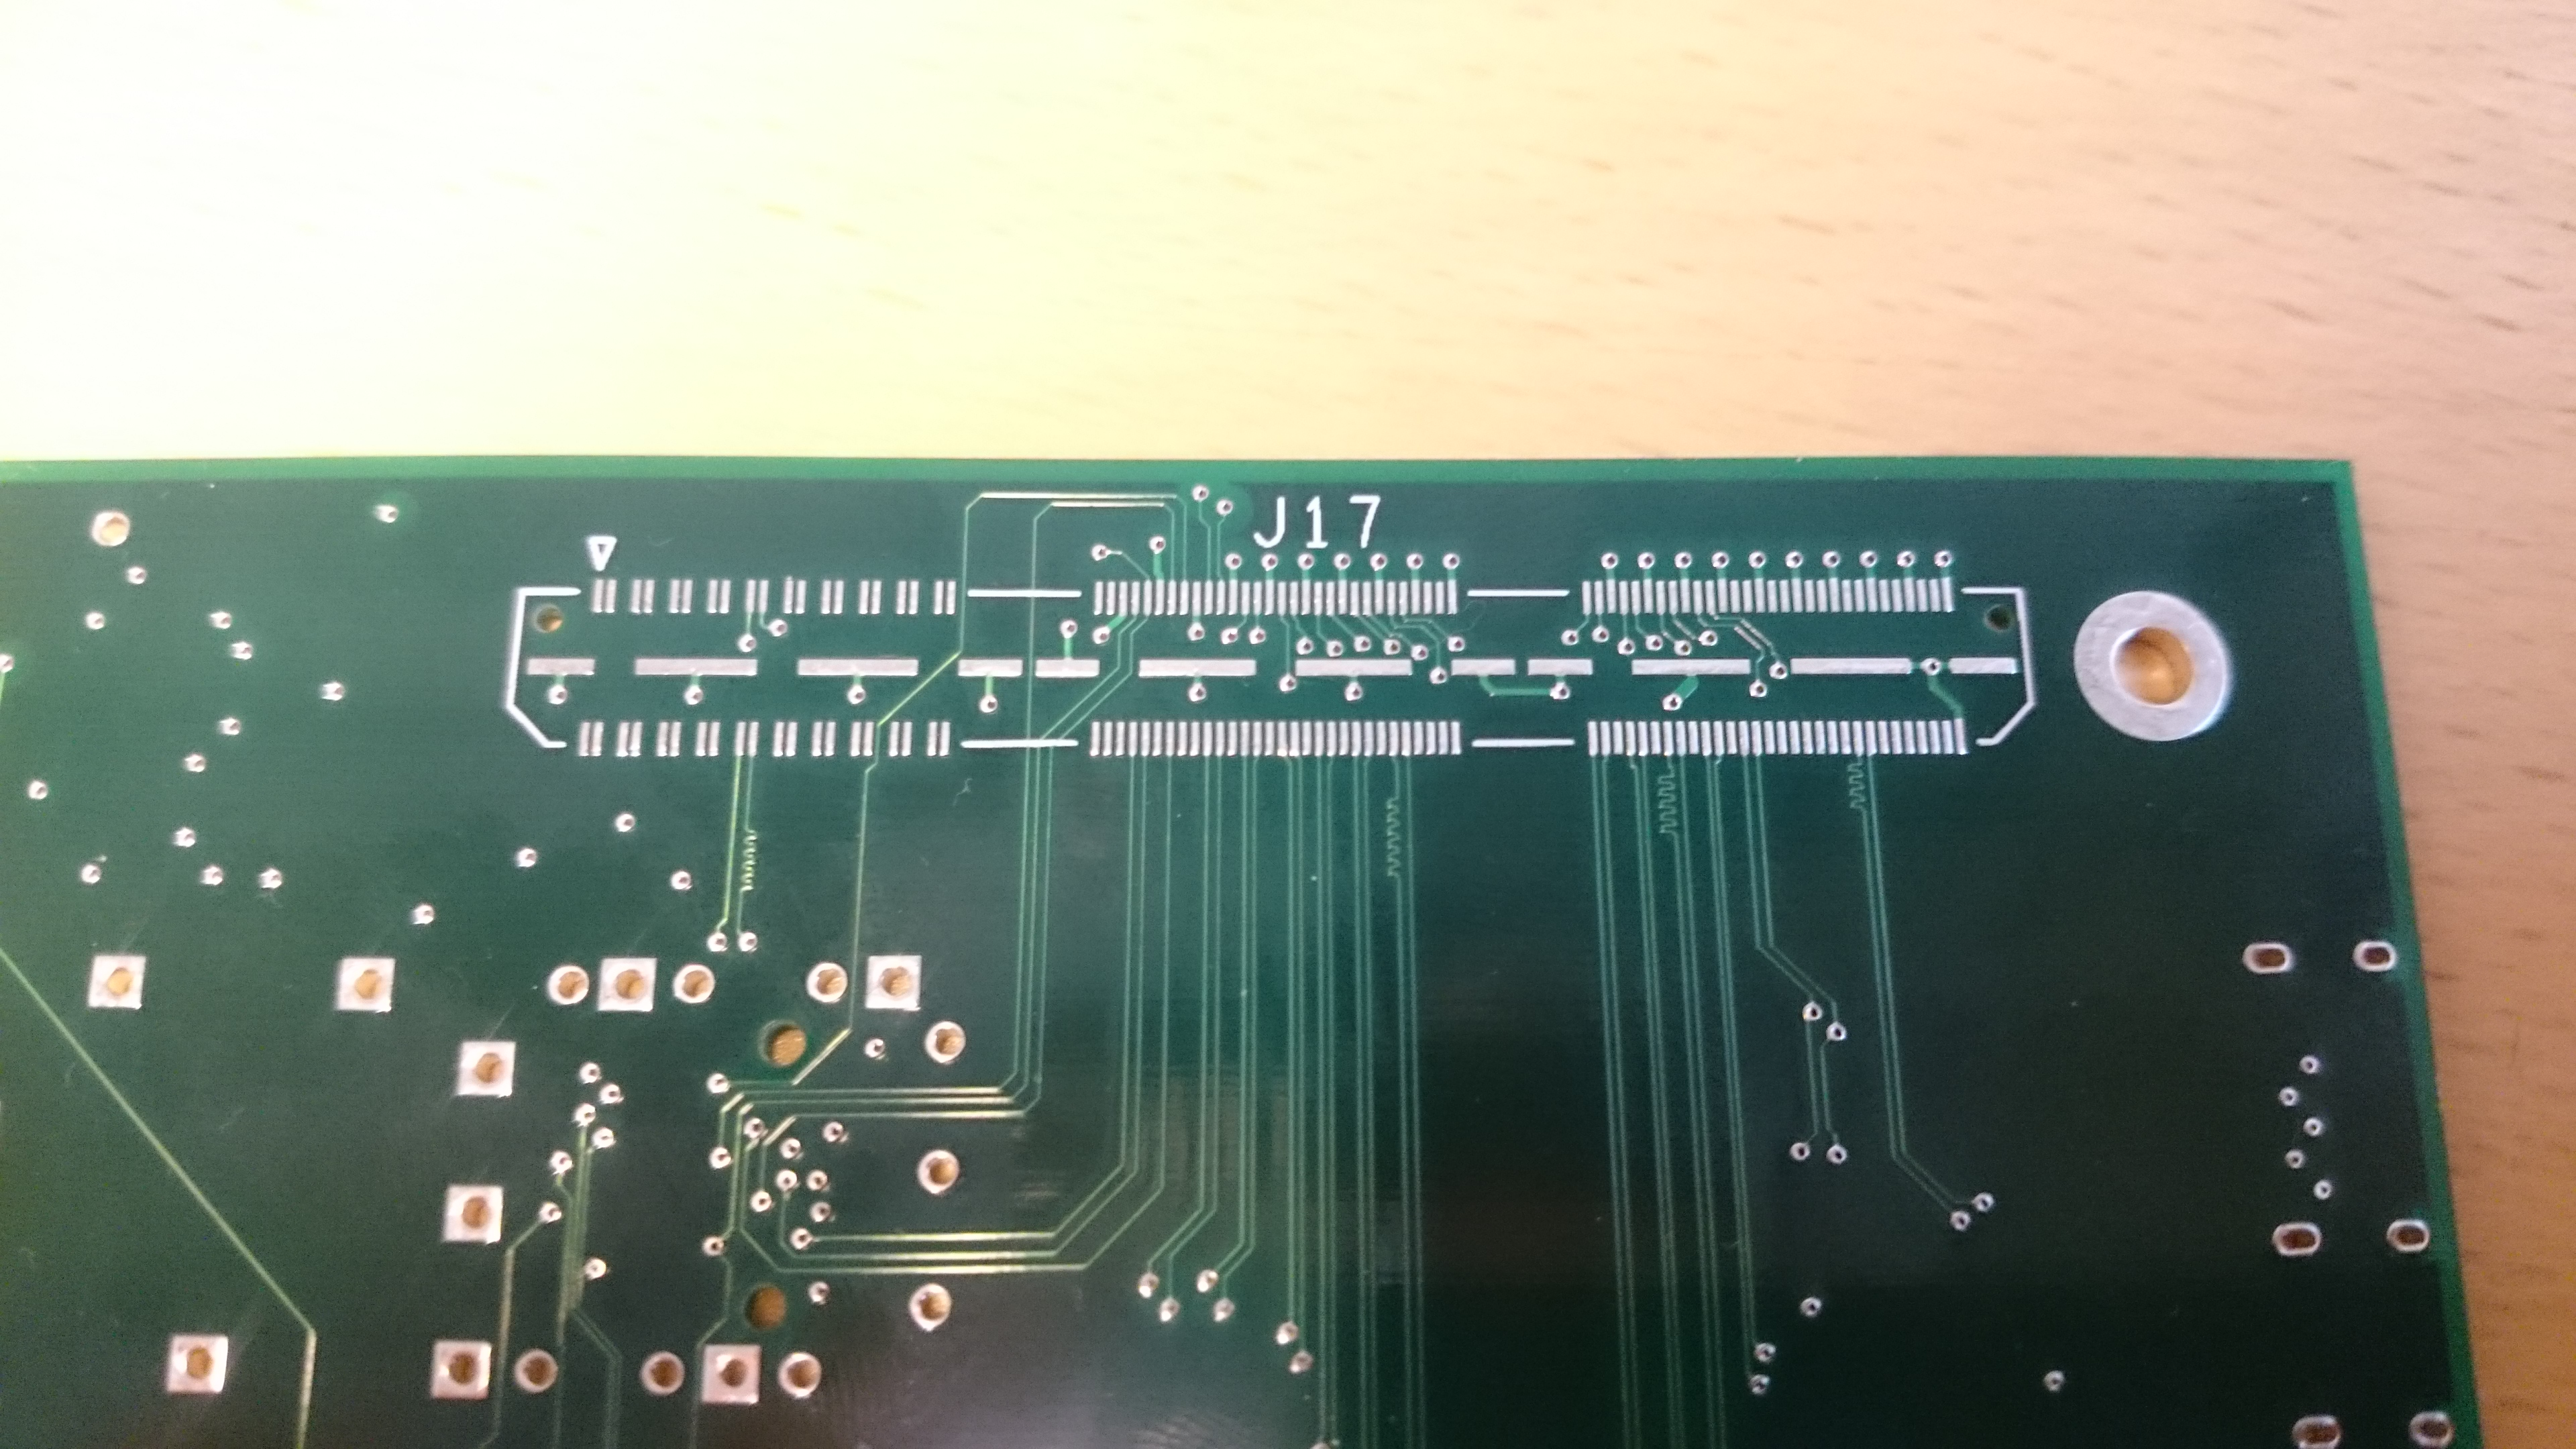
\includegraphics[width=0.4\paperwidth, trim={14cm 0cm 15cm 20cm}, clip]{../img/pcbbare2.JPG}
\end{backgroundblock}

\begin{textblock*}{\paperwidth}(6cm,7.5cm)
{\color{black} \Huge \textbf{$\rightarrow$}}
\end{textblock*}

\begin{backgroundblock}{2.0cm}{6.3cm}
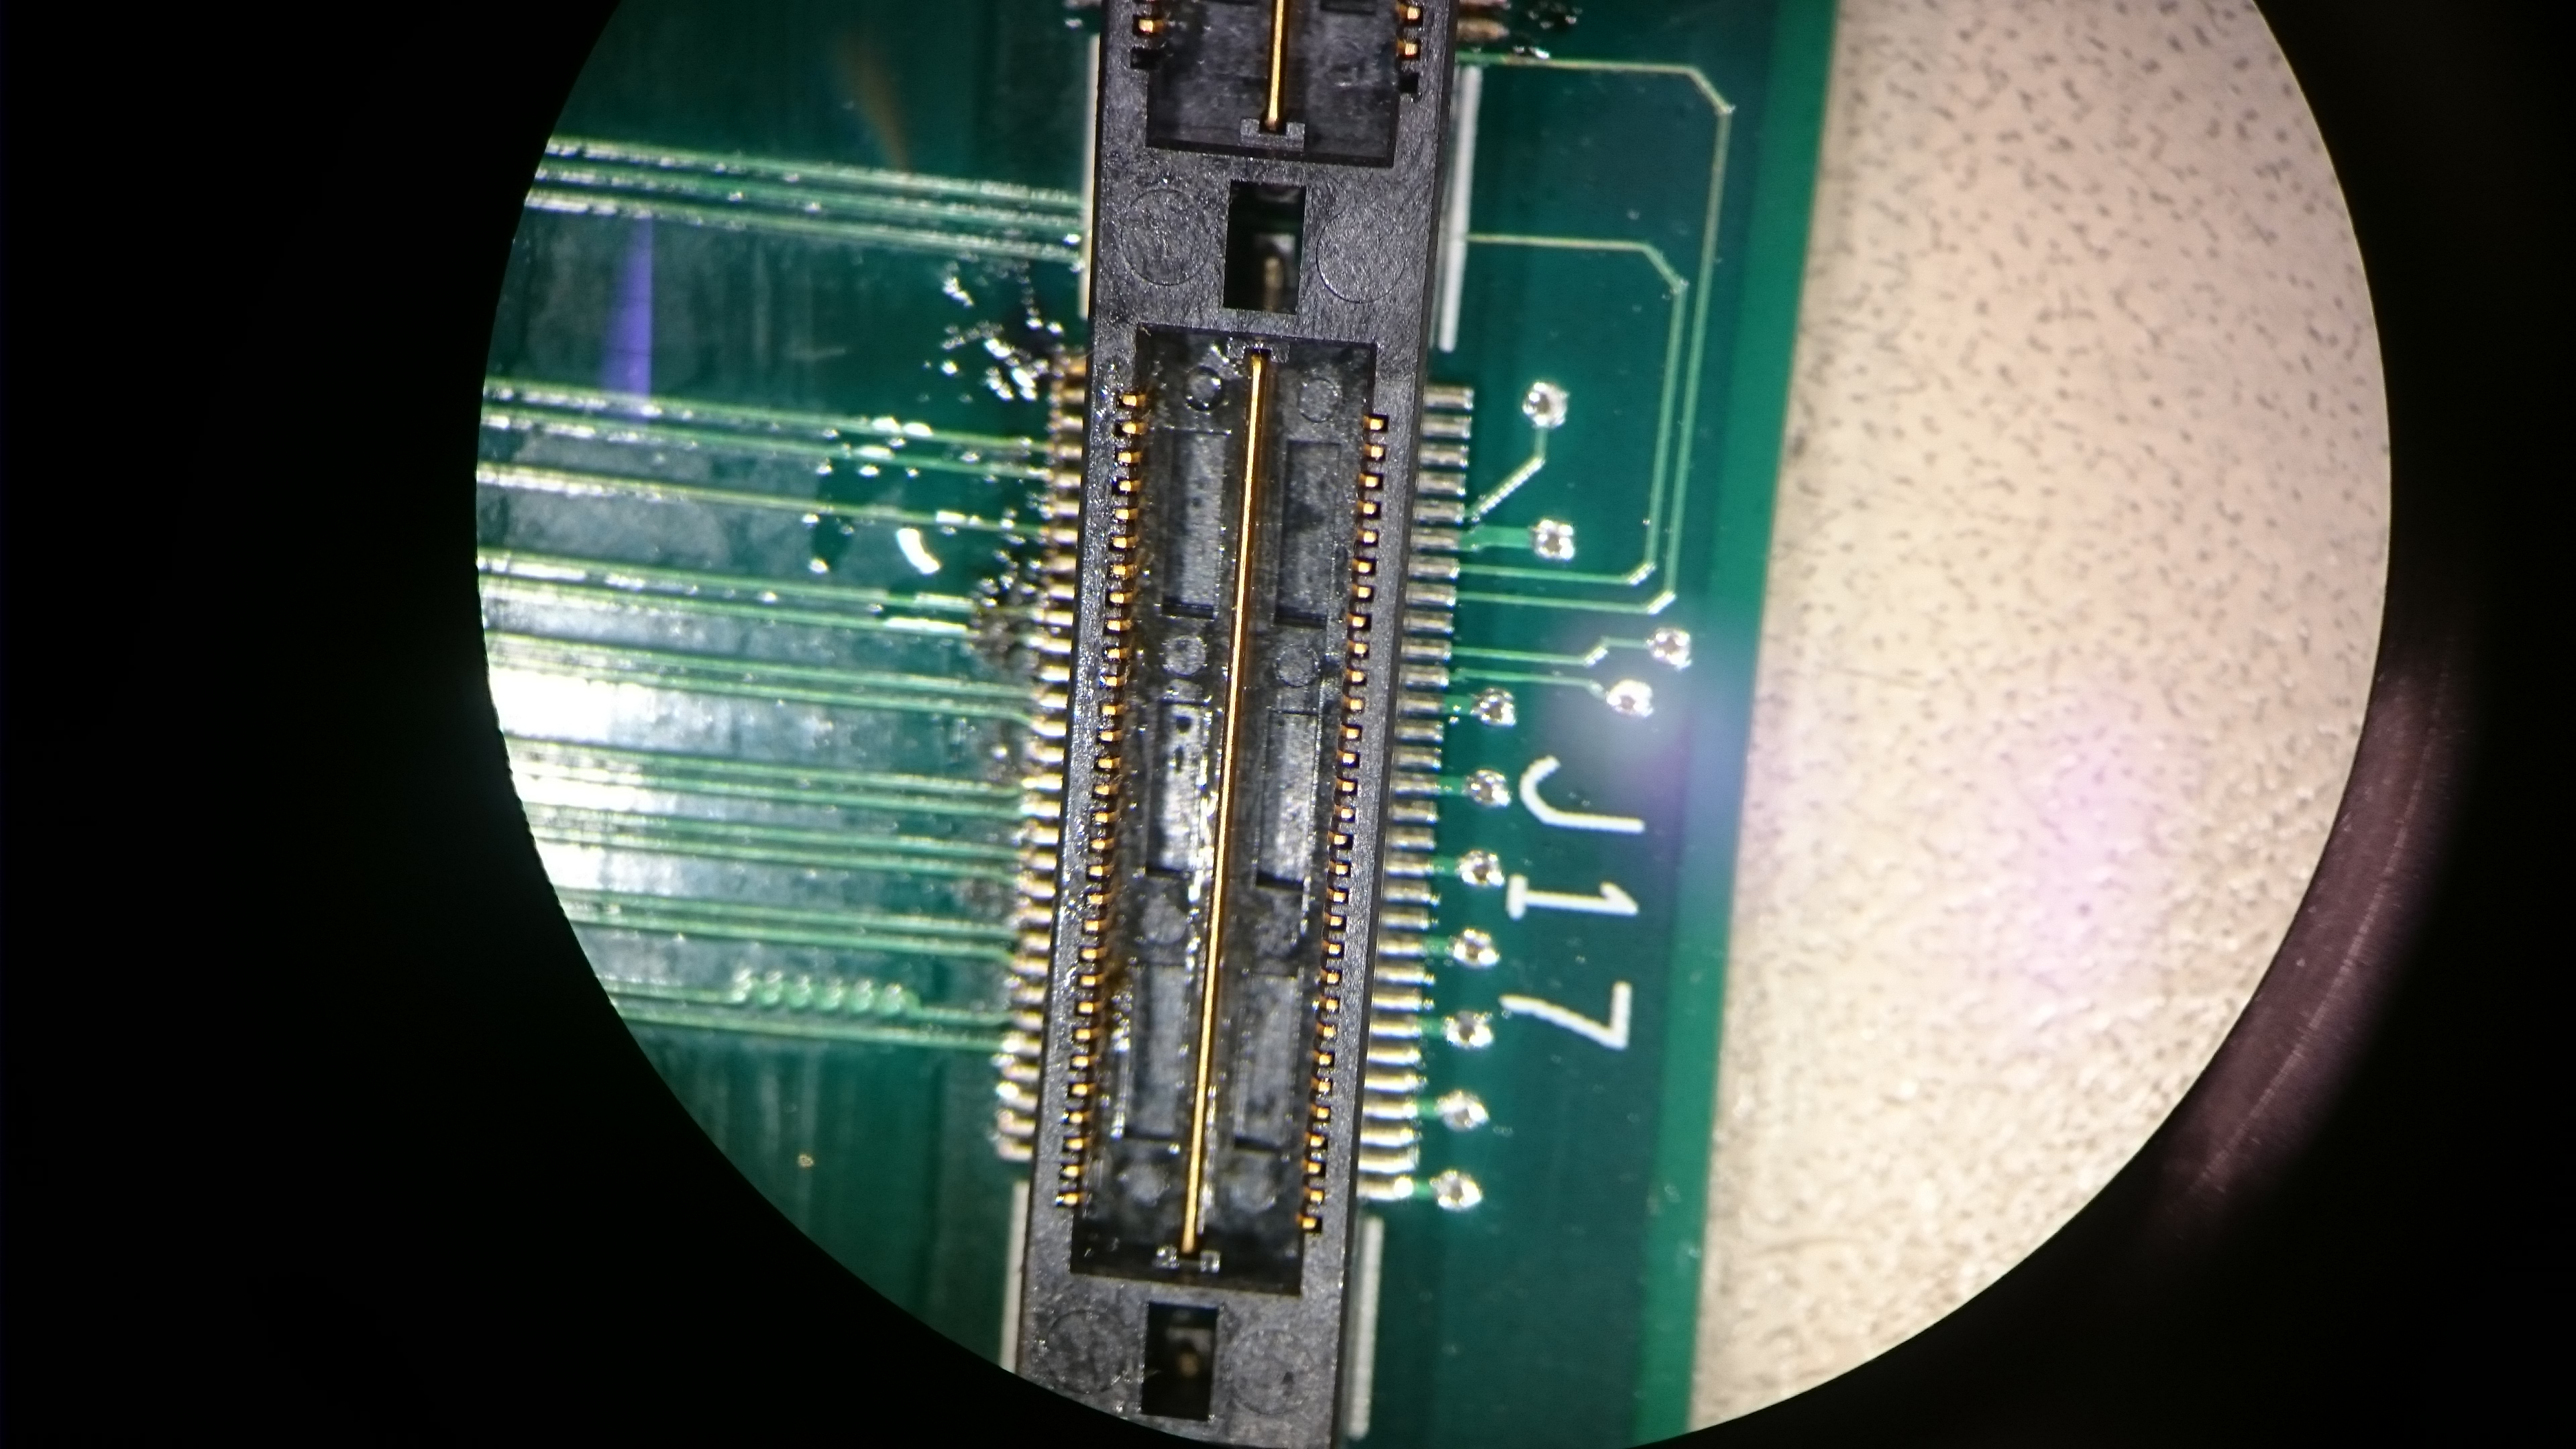
\includegraphics[width=0.2\paperwidth, trim={40cm 0cm 40cm 0cm}, clip, angle=90]{../img/pcbclose.JPG}
\end{backgroundblock}

\end{frame}
%------------------------------------------------

\begin{frame}[b]
\frametitle{Result}

\begin{backgroundblock}{2.0cm}{2.0cm}
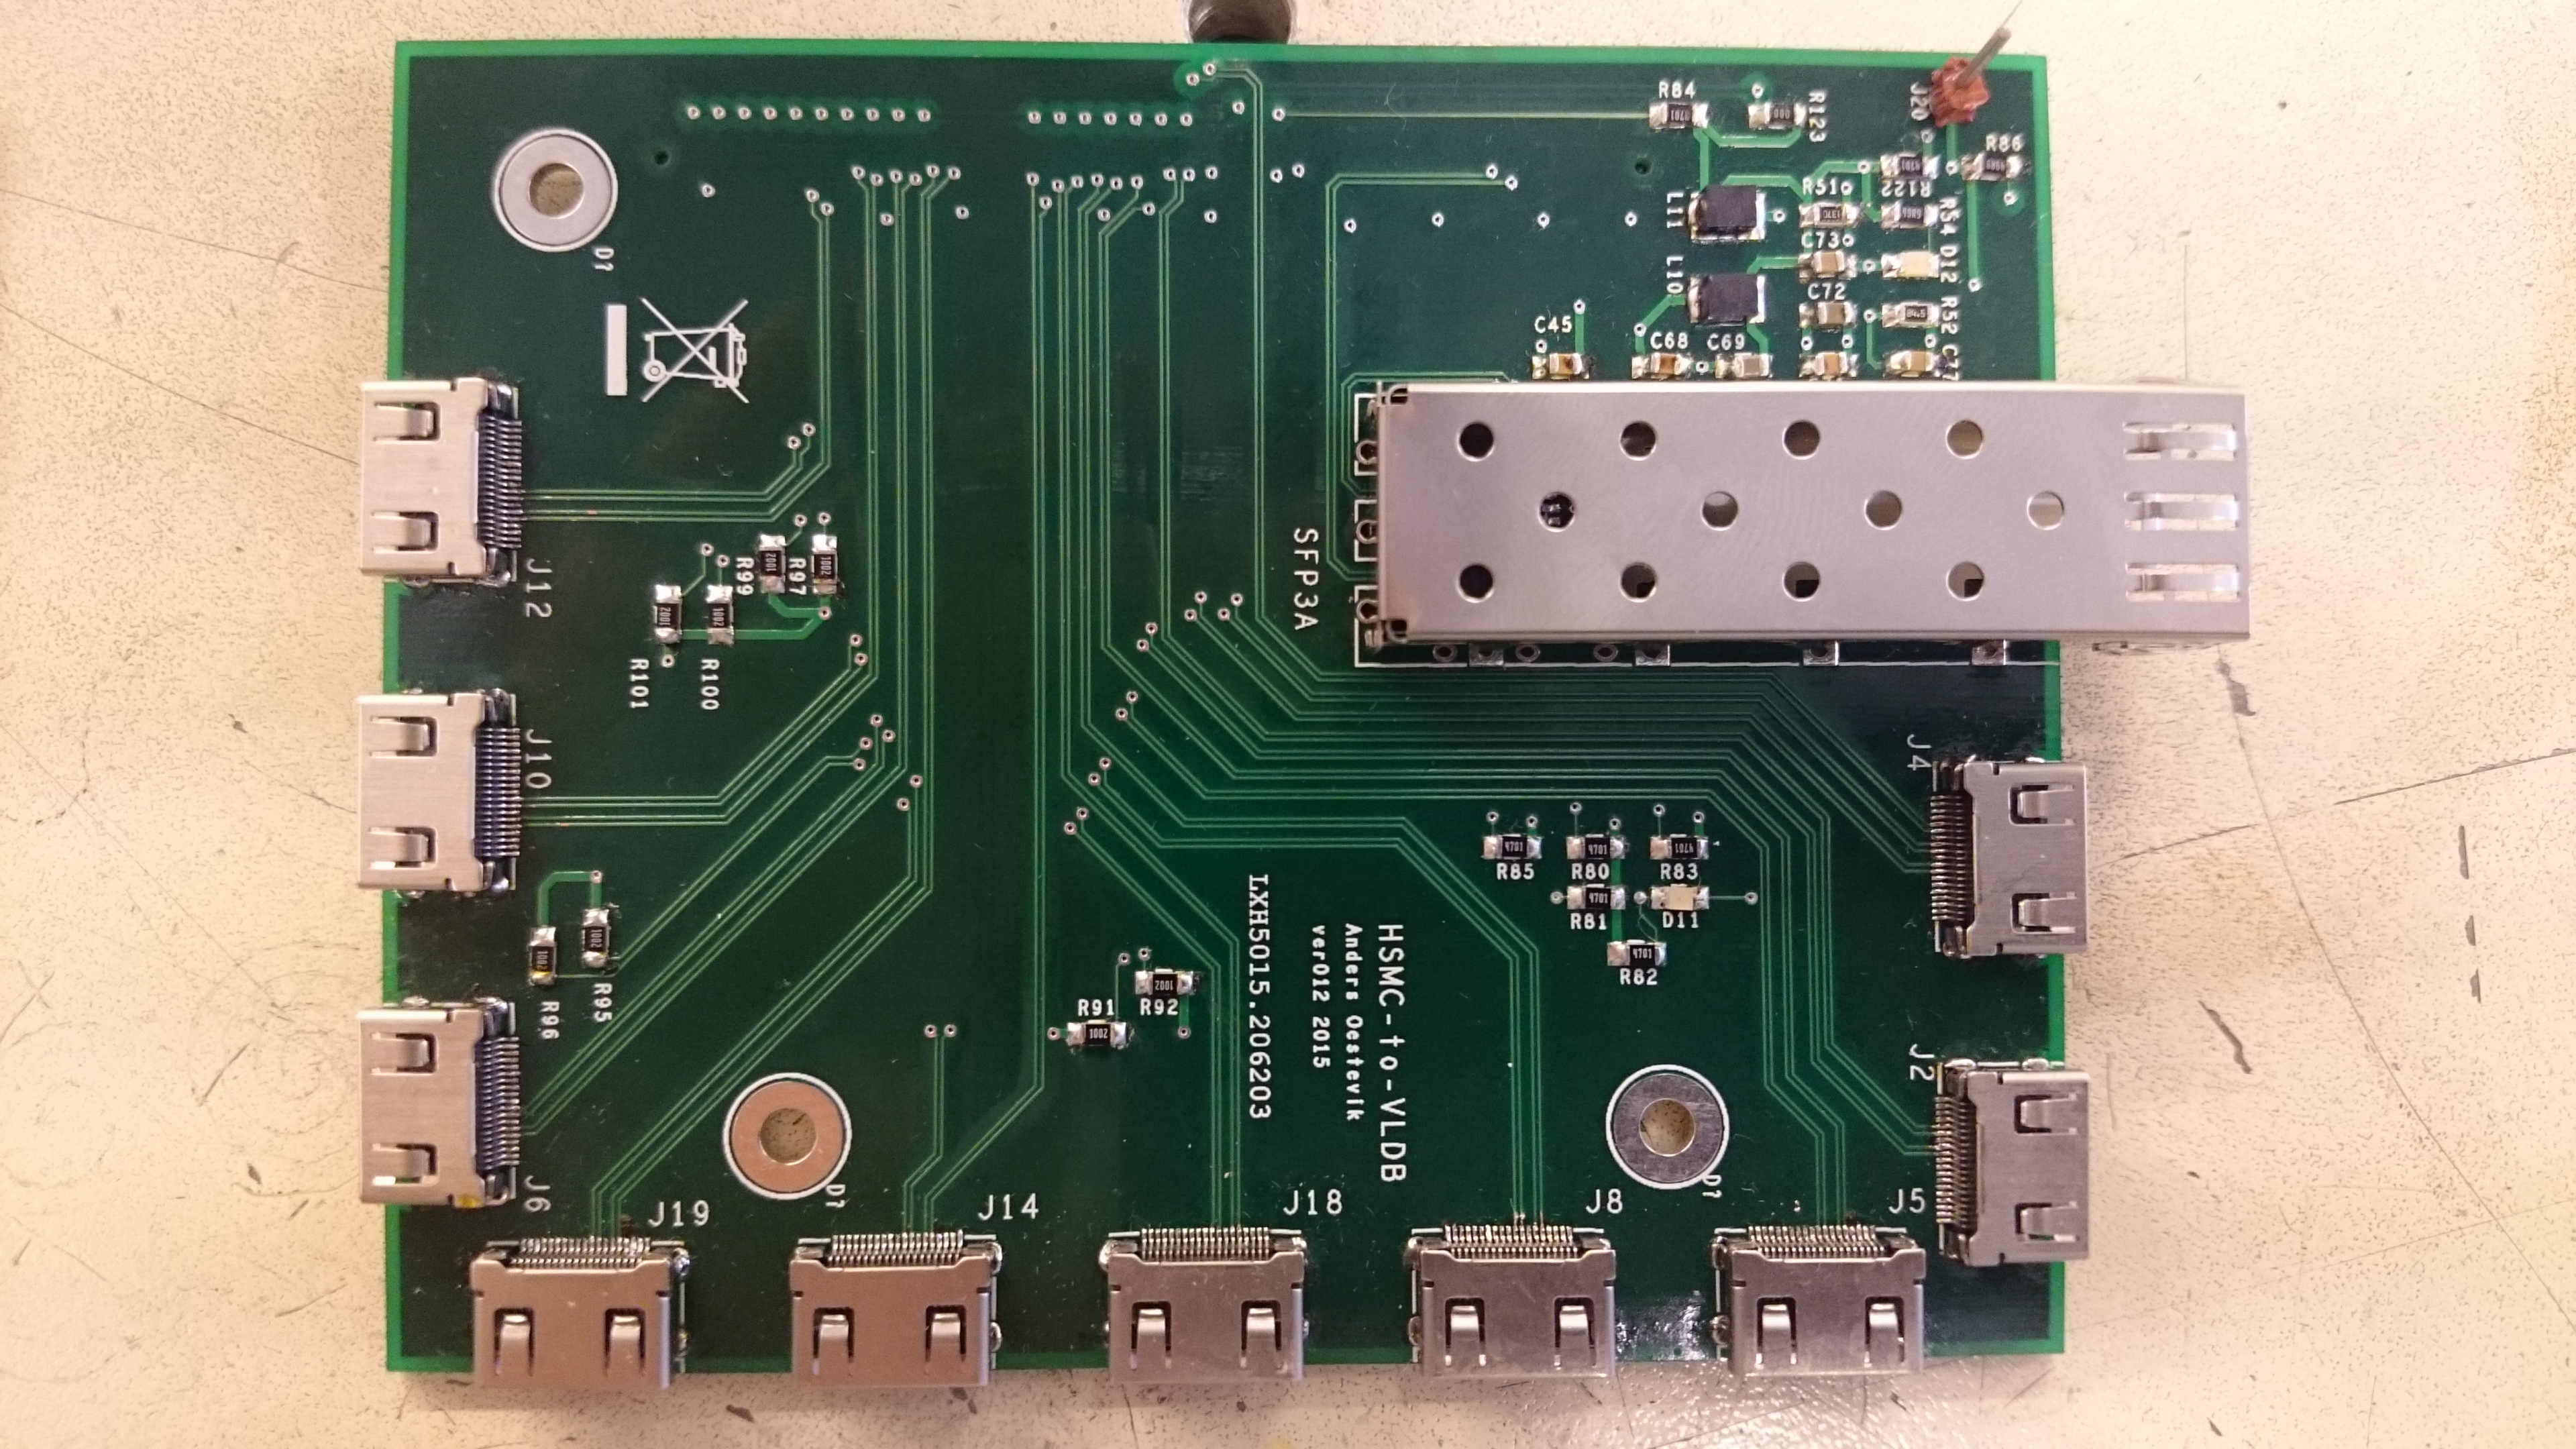
\includegraphics[width=0.7\paperwidth]{../img/pcb_1.JPG}
\end{backgroundblock}

\end{frame}
%------------------------------------------------

%------------------------------------------------
\section{GBT Control Software}
%------------------------------------------------
\subsection{Hardware}
\subsection{Software}
%------------------------------------------------

\begin{frame}[t]
\frametitle{GBT Control Software}

\begin{backgroundblock}{2cm}{5cm}
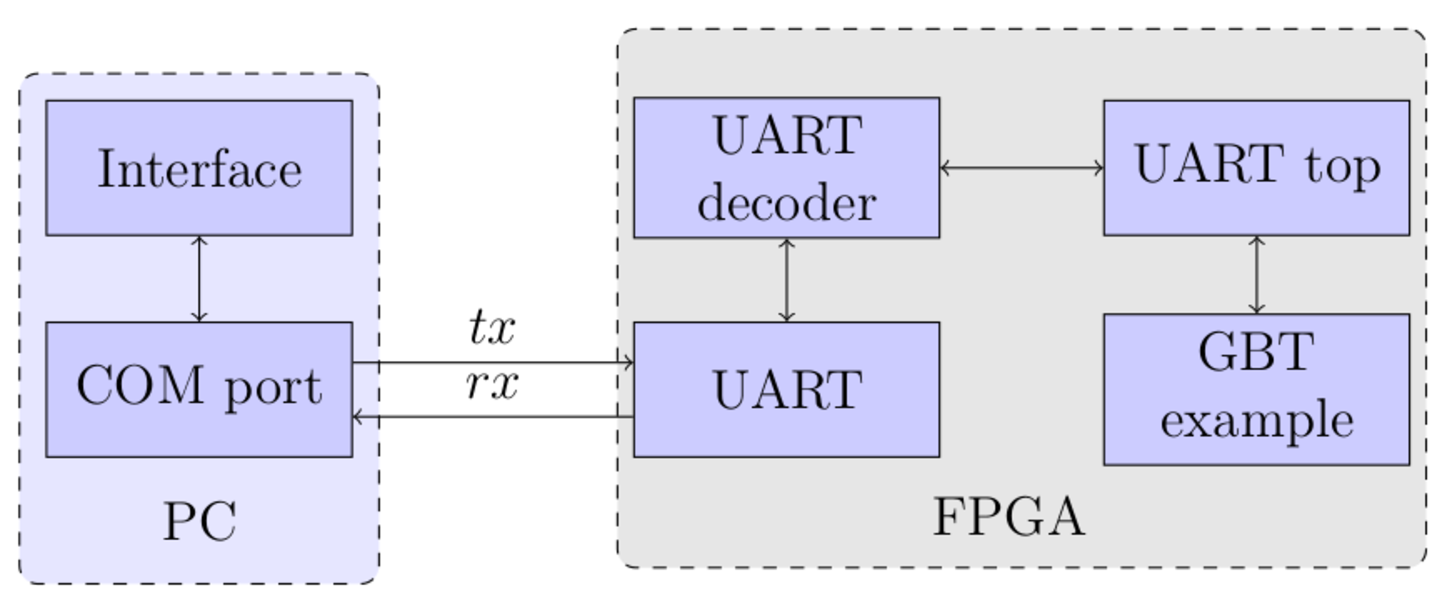
\includegraphics[width=0.6\paperwidth]{../img/softdia.pdf}
\end{backgroundblock}

\begin{backgroundblock}{5.5cm}{8.3cm}
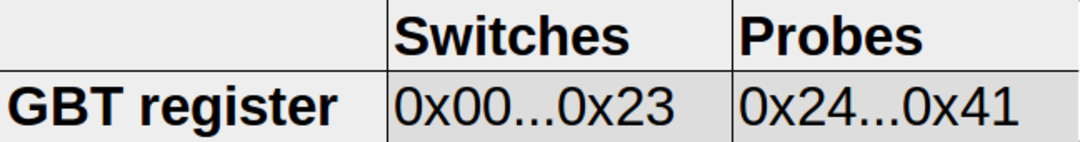
\includegraphics[width=0.3\paperwidth]{../img/gbtreg.pdf}
\end{backgroundblock}

\Large Specifications:\\
\normalsize
\begin{itemize}
\item Provide communication between PC and FPGA
\item Read and write GBT control signal information
\item Provide a simple User Interface	
\end{itemize}

\end{frame}
%------------------------------------------------

\begin{frame}[t]
\frametitle{Hardware}

\begin{backgroundblock}{2cm}{5cm}
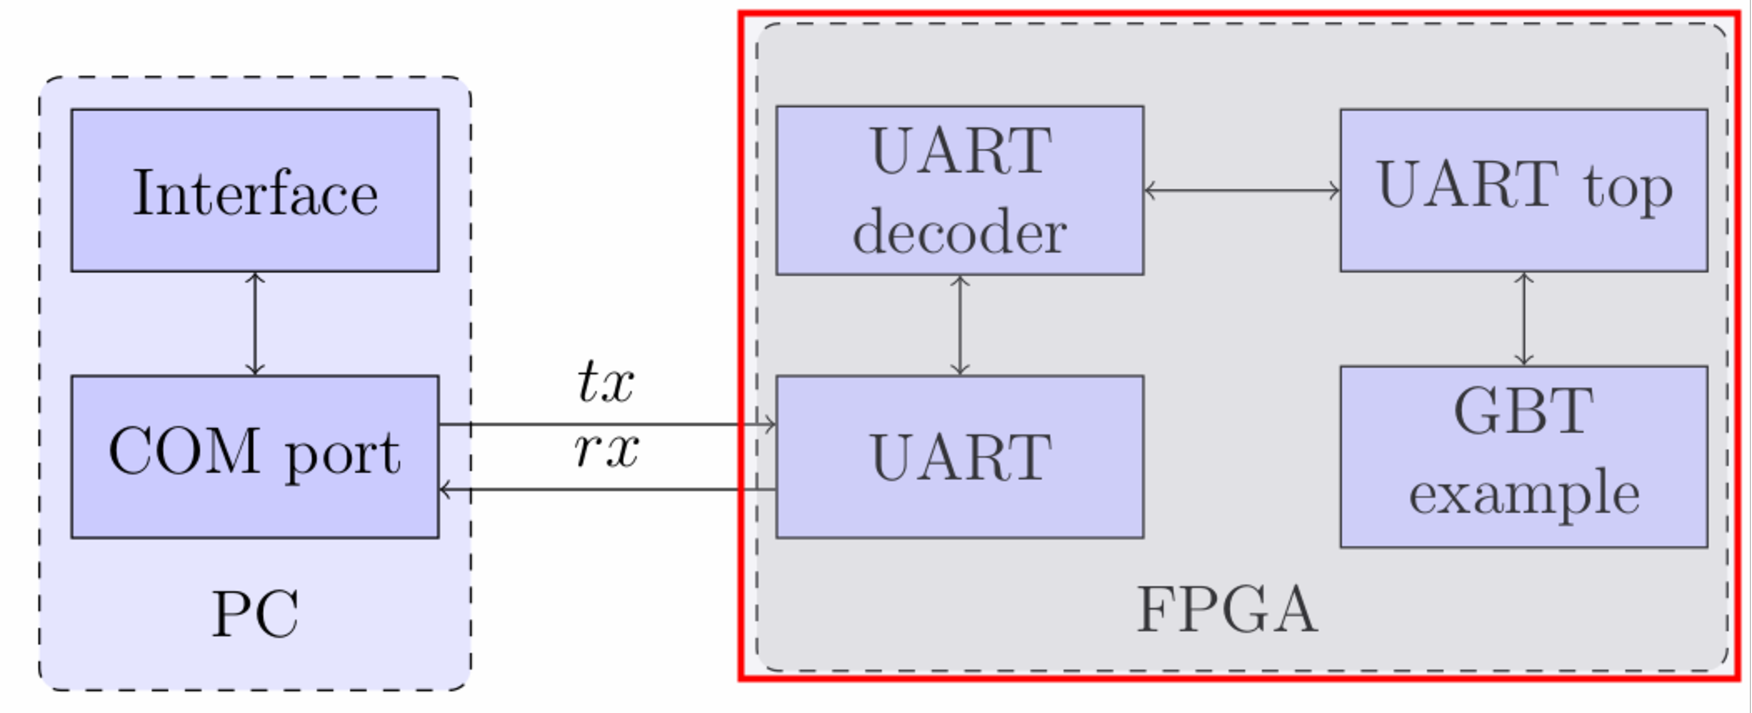
\includegraphics[width=0.6\paperwidth]{../img/harddia.pdf}
\end{backgroundblock}

\begin{backgroundblock}{5.5cm}{8.3cm}
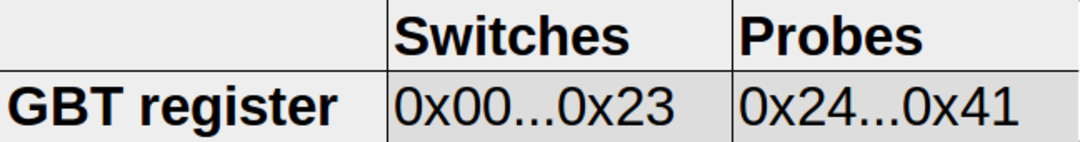
\includegraphics[width=0.3\paperwidth]{../img/gbtreg.pdf}
\end{backgroundblock}

\begin{itemize}
\item Treat incoming requests sent from PC
\item Components:
	\begin{itemize}
	\item UART (RX, TX, Buffers, baudrate generator)
	\item Decoder
	\end{itemize}
\item Goal: implement into GBT Example Design
\end{itemize}

\end{frame}
%------------------------------------------------

\begin{frame}[t]
\frametitle{UART}

\begin{backgroundblock}{1.5cm}{5cm}
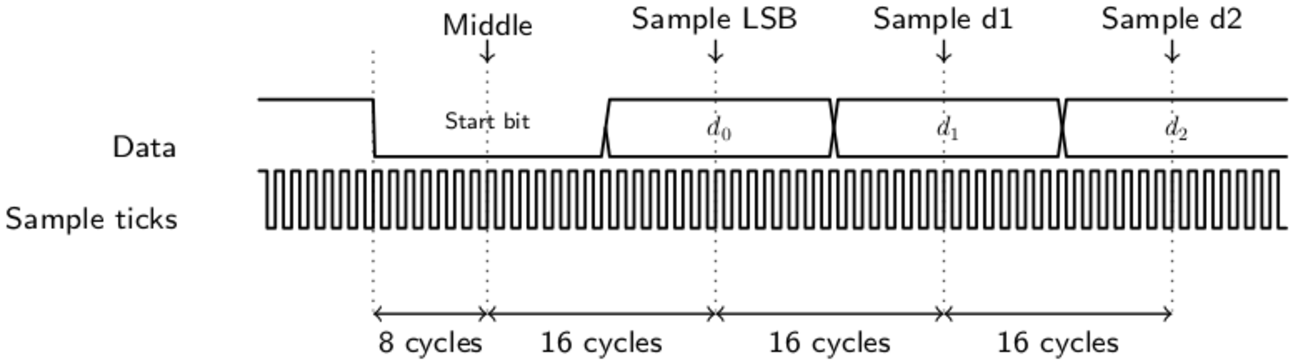
\includegraphics[width=0.7\paperwidth]{../img/oversamp.pdf}
\end{backgroundblock}

\begin{itemize}
\item Synchronisation $\rightarrow$ Oversampling
\item $16 \times baudrate$ - fixed
\item Stores bytes in FIFO-buffers
\item $19200-8-N-1~ \rightarrow 307200$ sample clock
\end{itemize}

\end{frame}
%------------------------------------------------

\begin{frame}[t]
\frametitle{Decoder}

\begin{backgroundblock}{-0.1cm}{5cm}
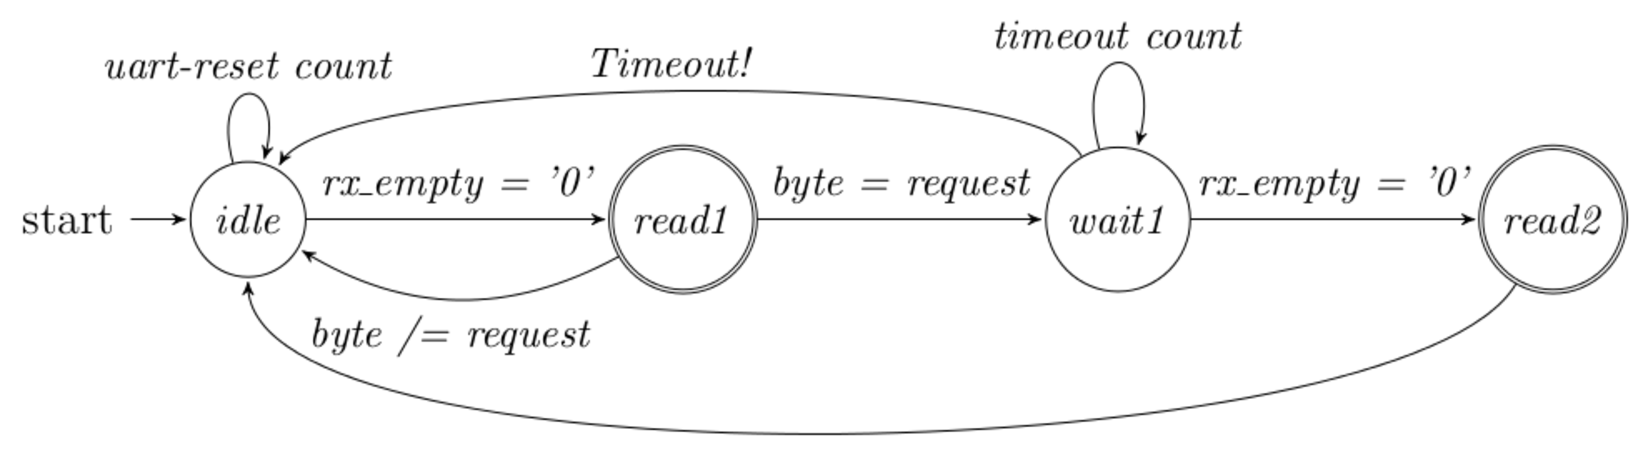
\includegraphics[width=1\paperwidth]{../img/statedec.pdf}
\end{backgroundblock}

\begin{columns}[c] %The "c" option specifies centered vertical alignment while the "t" option is used for top vertical alignment

\column{.45\textwidth} % Left column and width
\begin{itemize}
\item Requests:
	\begin{itemize}
	\item read $\rightarrow$ 0xDD
	\item write 0 $\rightarrow$ 0xEE
	\item write 1 $\rightarrow$ 0xFF
	\end{itemize}
\end{itemize}

\column{.5\textwidth} % Right column and width
\begin{itemize}
\item Legal addresses:
	\begin{itemize}
	\item 0x00 $\rightarrow$ 0x41
	\end{itemize}
\item Bytes sent to PC:
	\begin{itemize}
	\item 0x00 $\rightarrow$ 0xC1
	\end{itemize}	
\end{itemize}

\end{columns}

\end{frame}
%------------------------------------------------

\begin{frame}
\frametitle{Software}

\begin{backgroundblock}{2cm}{3cm}
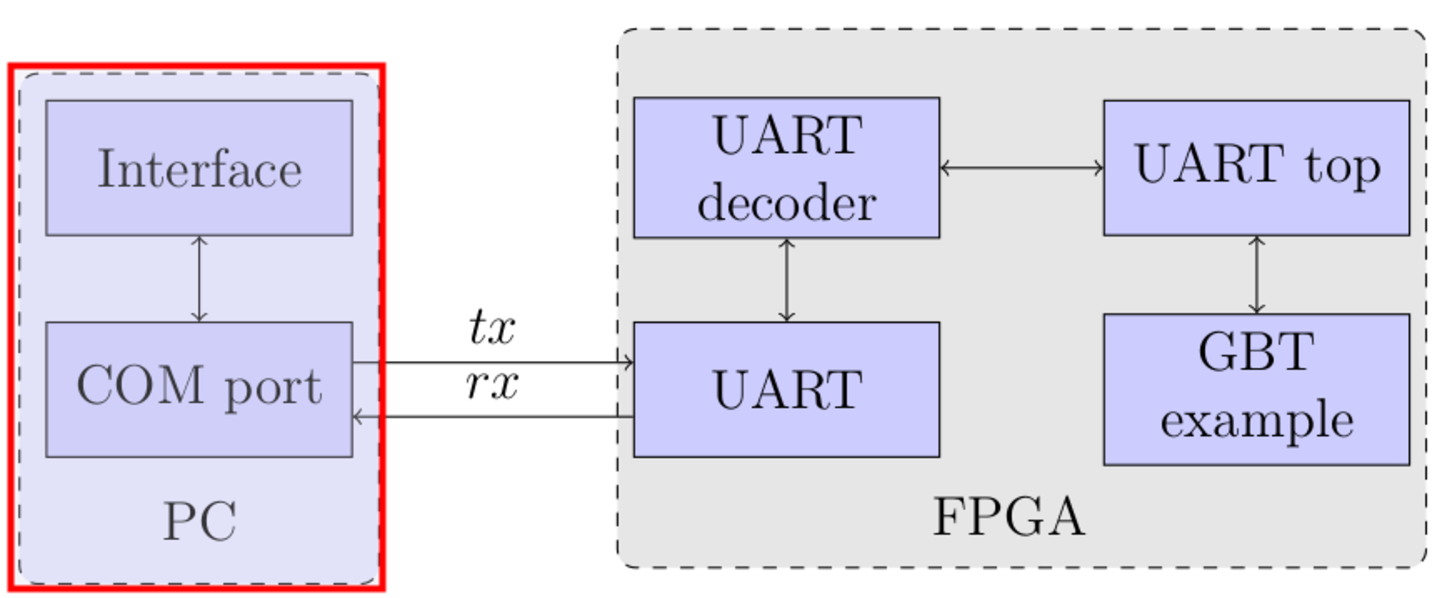
\includegraphics[width=0.6\paperwidth]{../img/softdia2.pdf}
\end{backgroundblock}

\begin{backgroundblock}{5.5cm}{6.3cm}
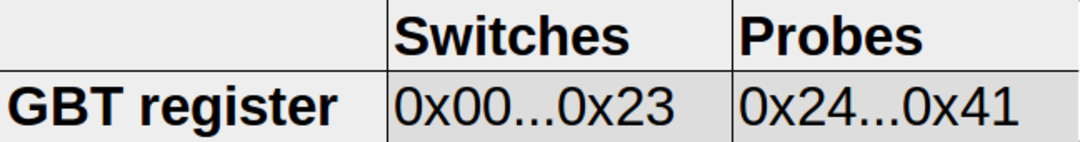
\includegraphics[width=0.3\paperwidth]{../img/gbtreg.pdf}
\end{backgroundblock}

\end{frame}
%------------------------------------------------

\begin{frame}
\frametitle{Software}

\Large Modules:\\
\normalsize
\begin{itemize}
\item Send/Receive
	\begin{itemize}
	\item RS-232 library
	\item Continuously transmits pattern to GBT-registers
	\item Reads it back for transmit confirmation
	\end{itemize}
\item User Interface
	\begin{itemize}
	\item ncurses library
	\item User commands: write, read, status, open, close, exit
	\item Dummy registers instead of real GBT-registers
	\end{itemize}
\item GBT register data $\rightarrow$ stored and maintained using a custom \textit{Signals}-library
\end{itemize}

\end{frame}
%------------------------------------------------

\begin{frame}[t]
\frametitle{Send/Receive Module}

\begin{backgroundblock}{4.5cm}{3cm}
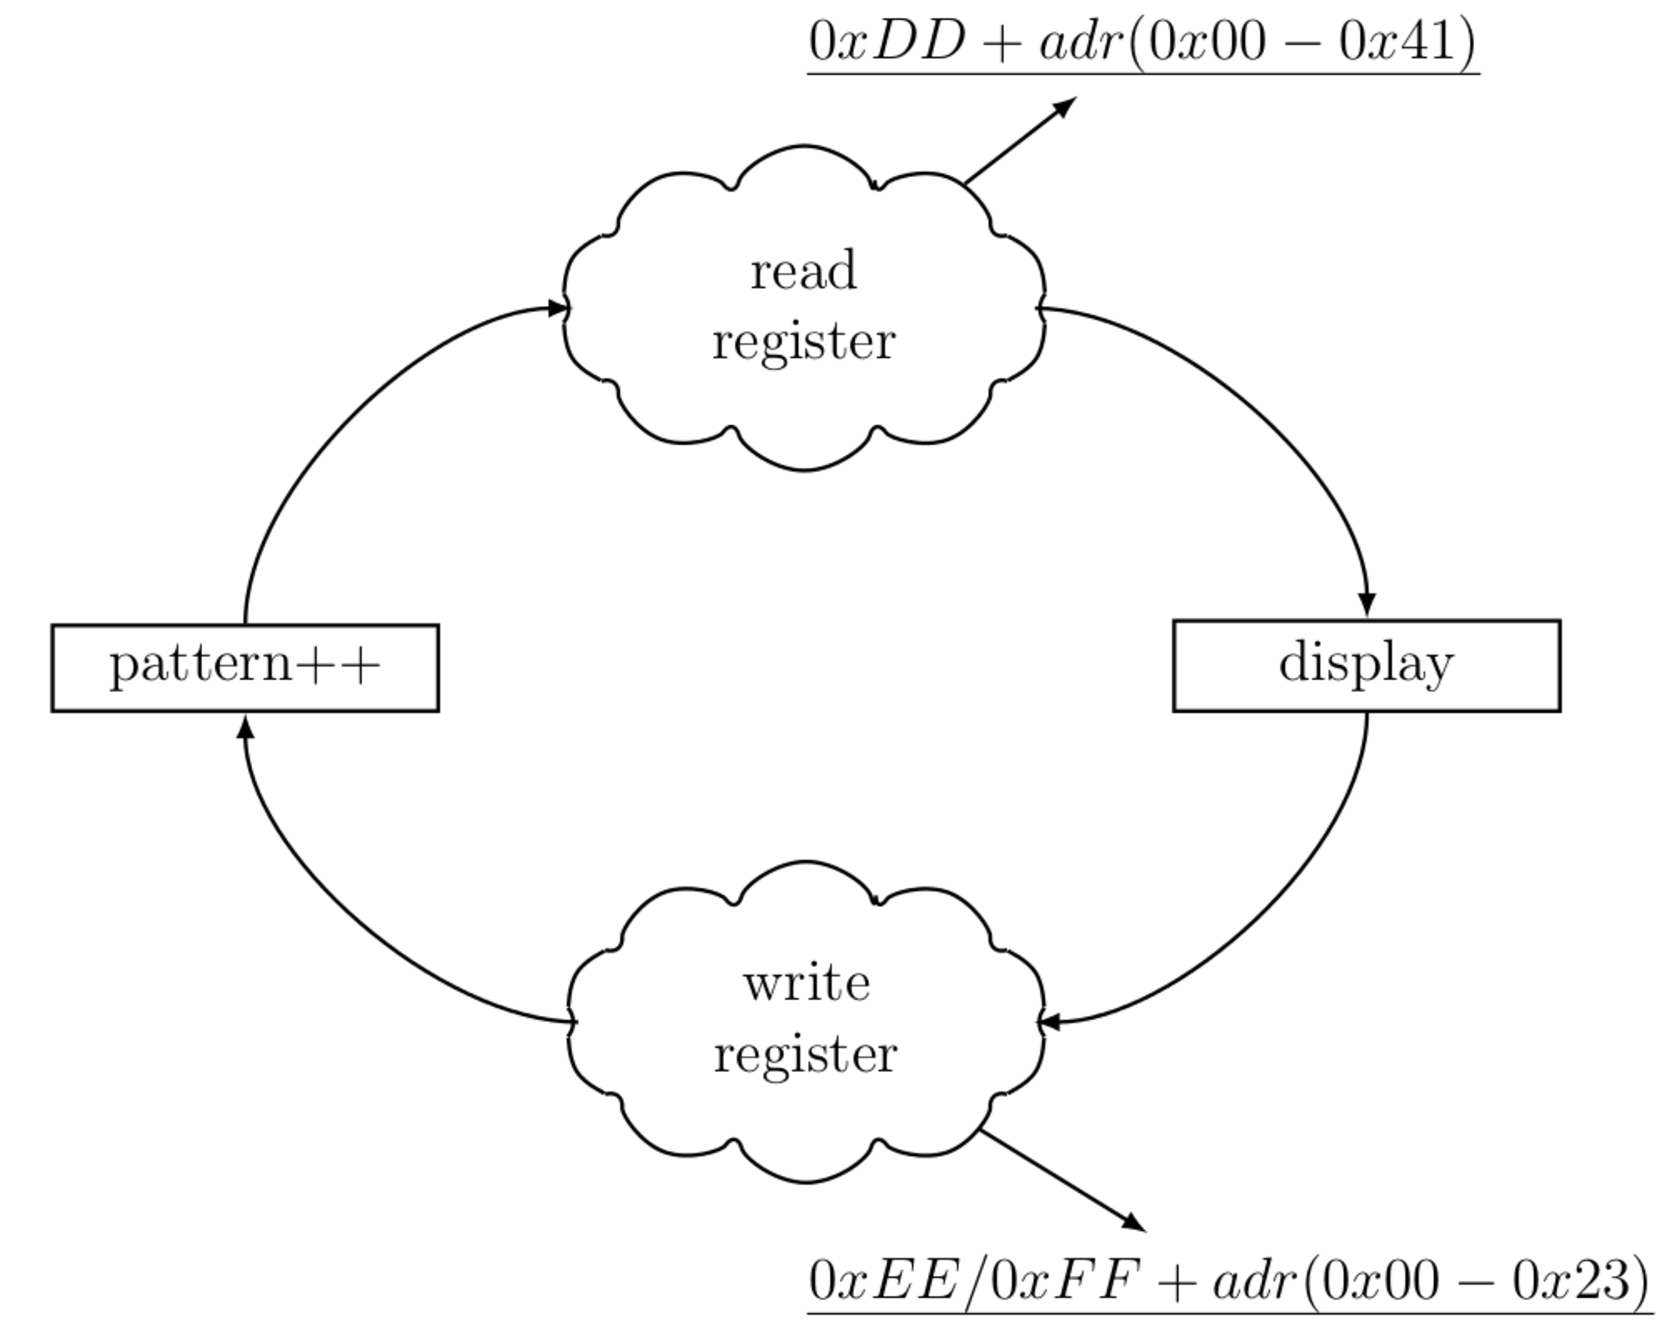
\includegraphics[width=0.6\paperwidth]{../img/prgcycle2.pdf}
\end{backgroundblock}

\begin{itemize}
\item Read: transmit 2 bytes, receive 1 byte
\item Write: transmit 2 bytes
\item 2D-array with "patterns"
\item COM-port $\leftarrow\rightarrow$ FPGA
\end{itemize}

\end{frame}
%------------------------------------------------

% \begin{frame}[t]
% \frametitle{Read register}

% \begin{backgroundblock}{1.5cm}{2cm}
% 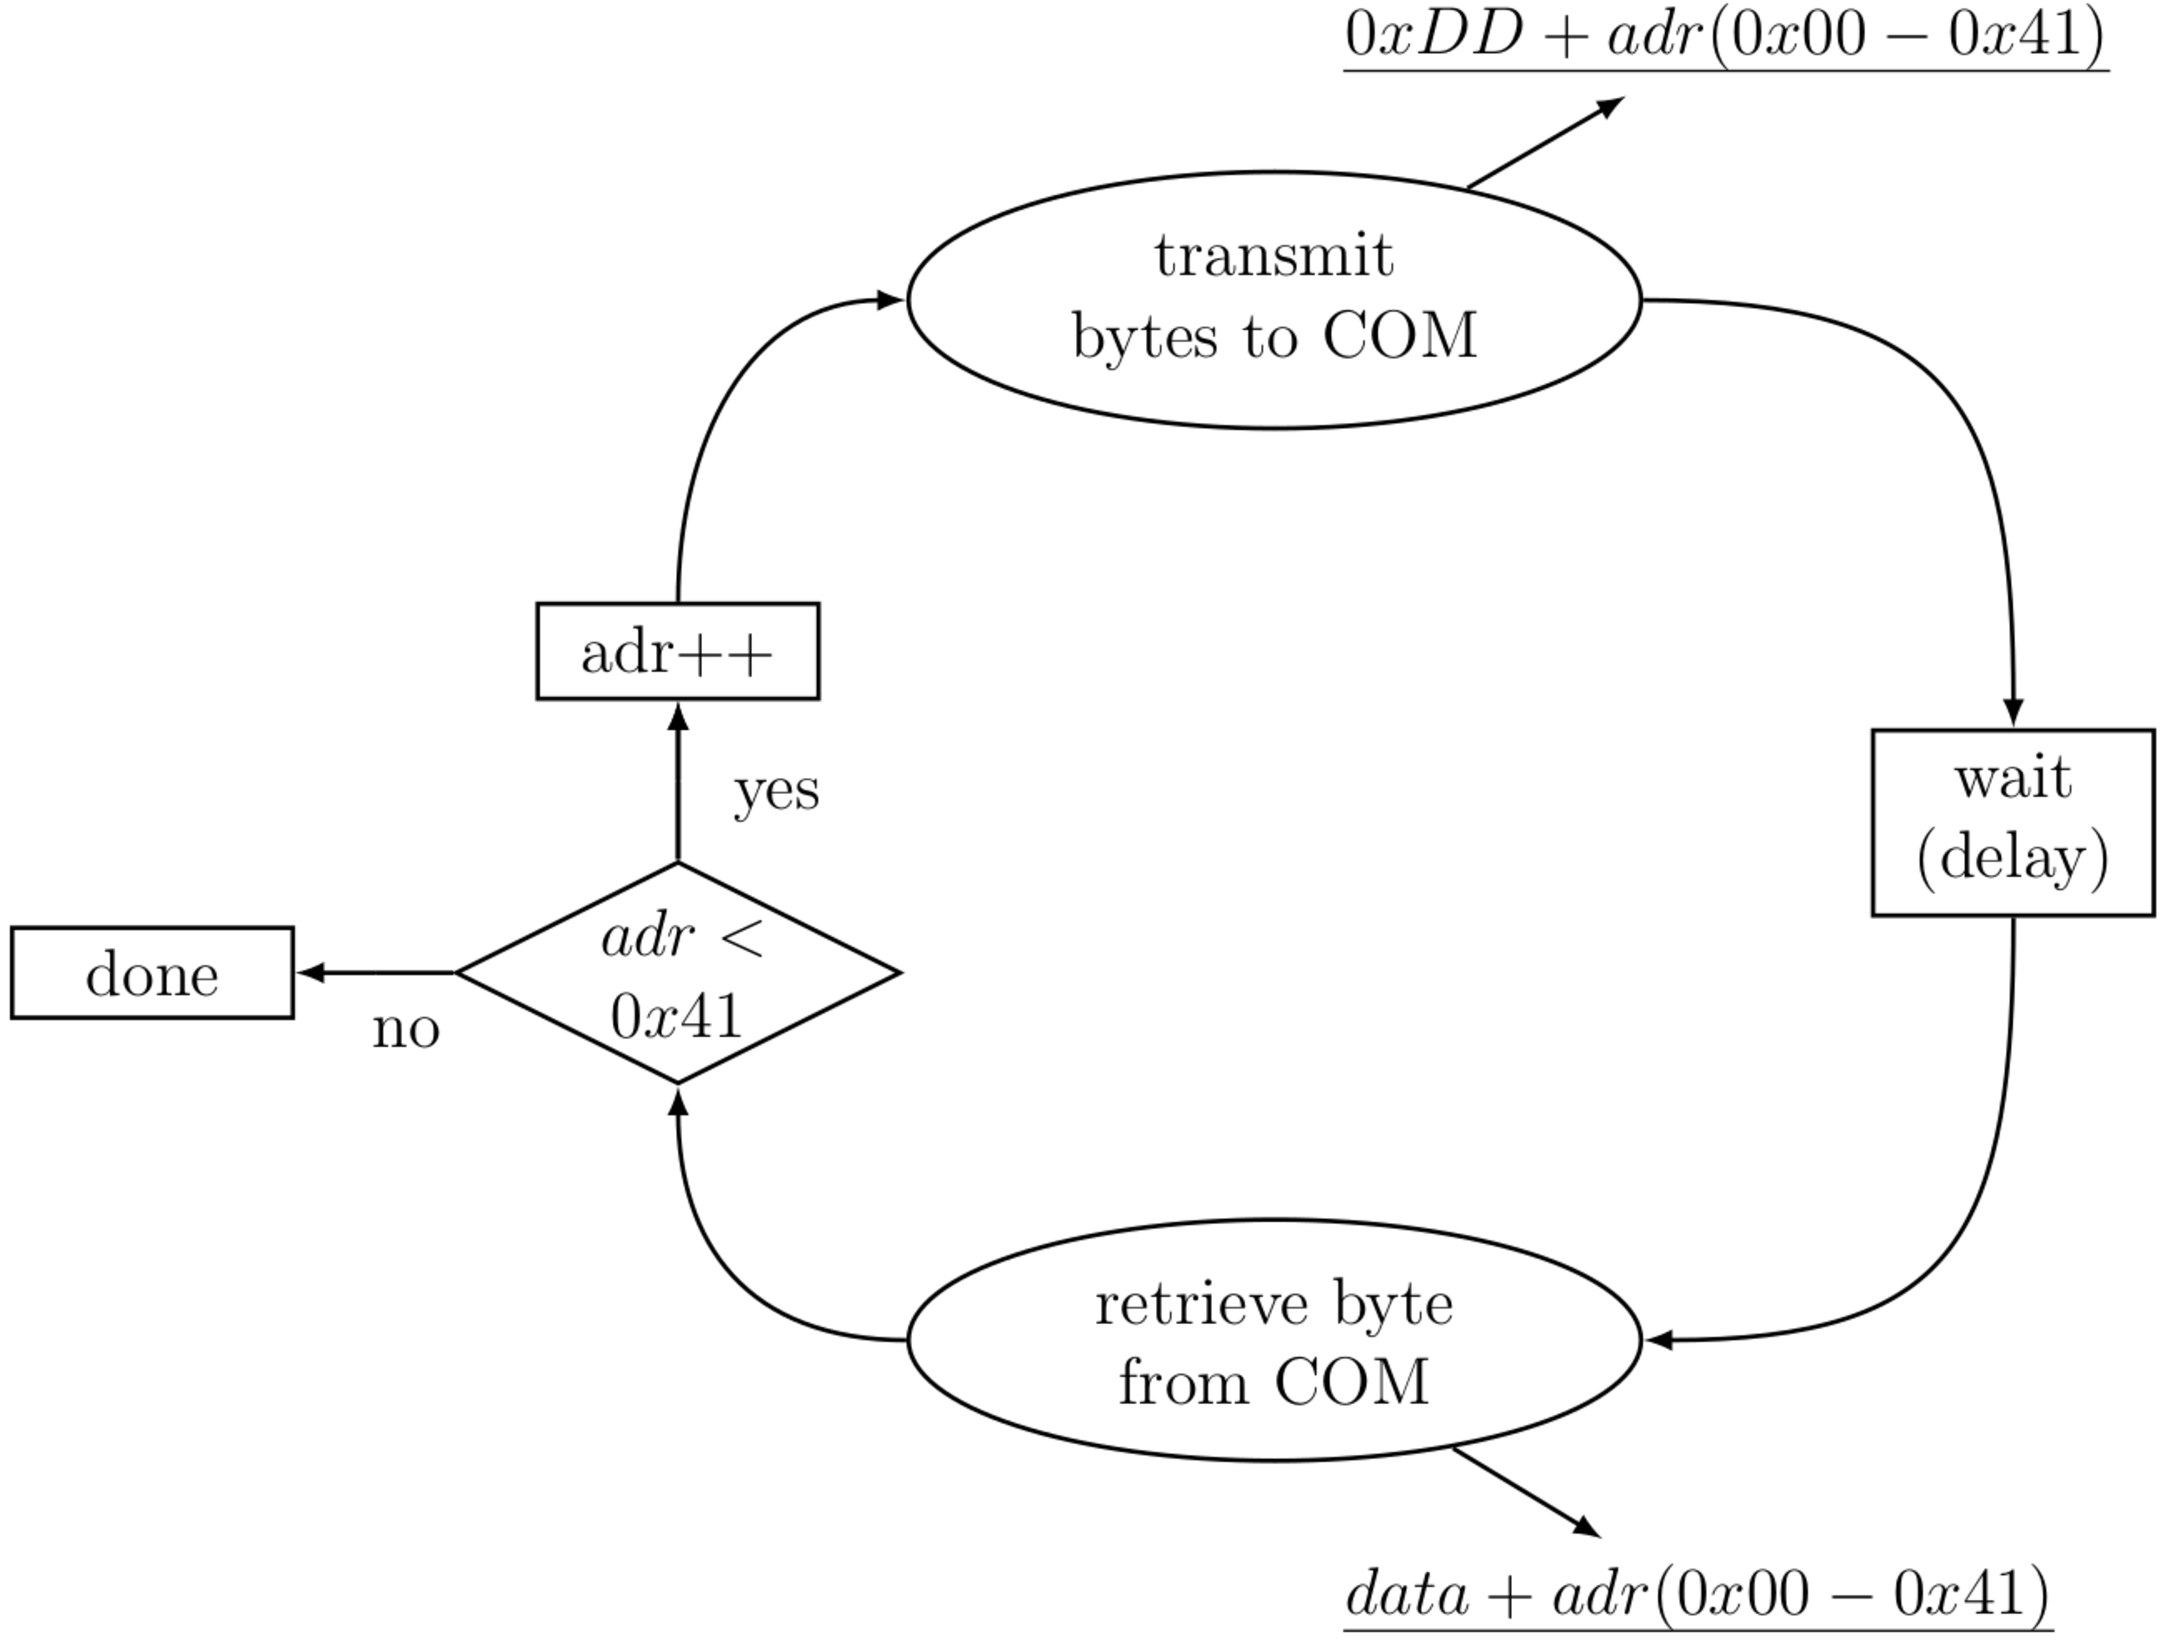
\includegraphics[width=0.7\paperwidth]{../img/rx_cycle.pdf}
% \end{backgroundblock}

% \end{frame}
% %------------------------------------------------

% \begin{frame}[t]
% \frametitle{Write register}

% \begin{backgroundblock}{1.5cm}{3cm}
% 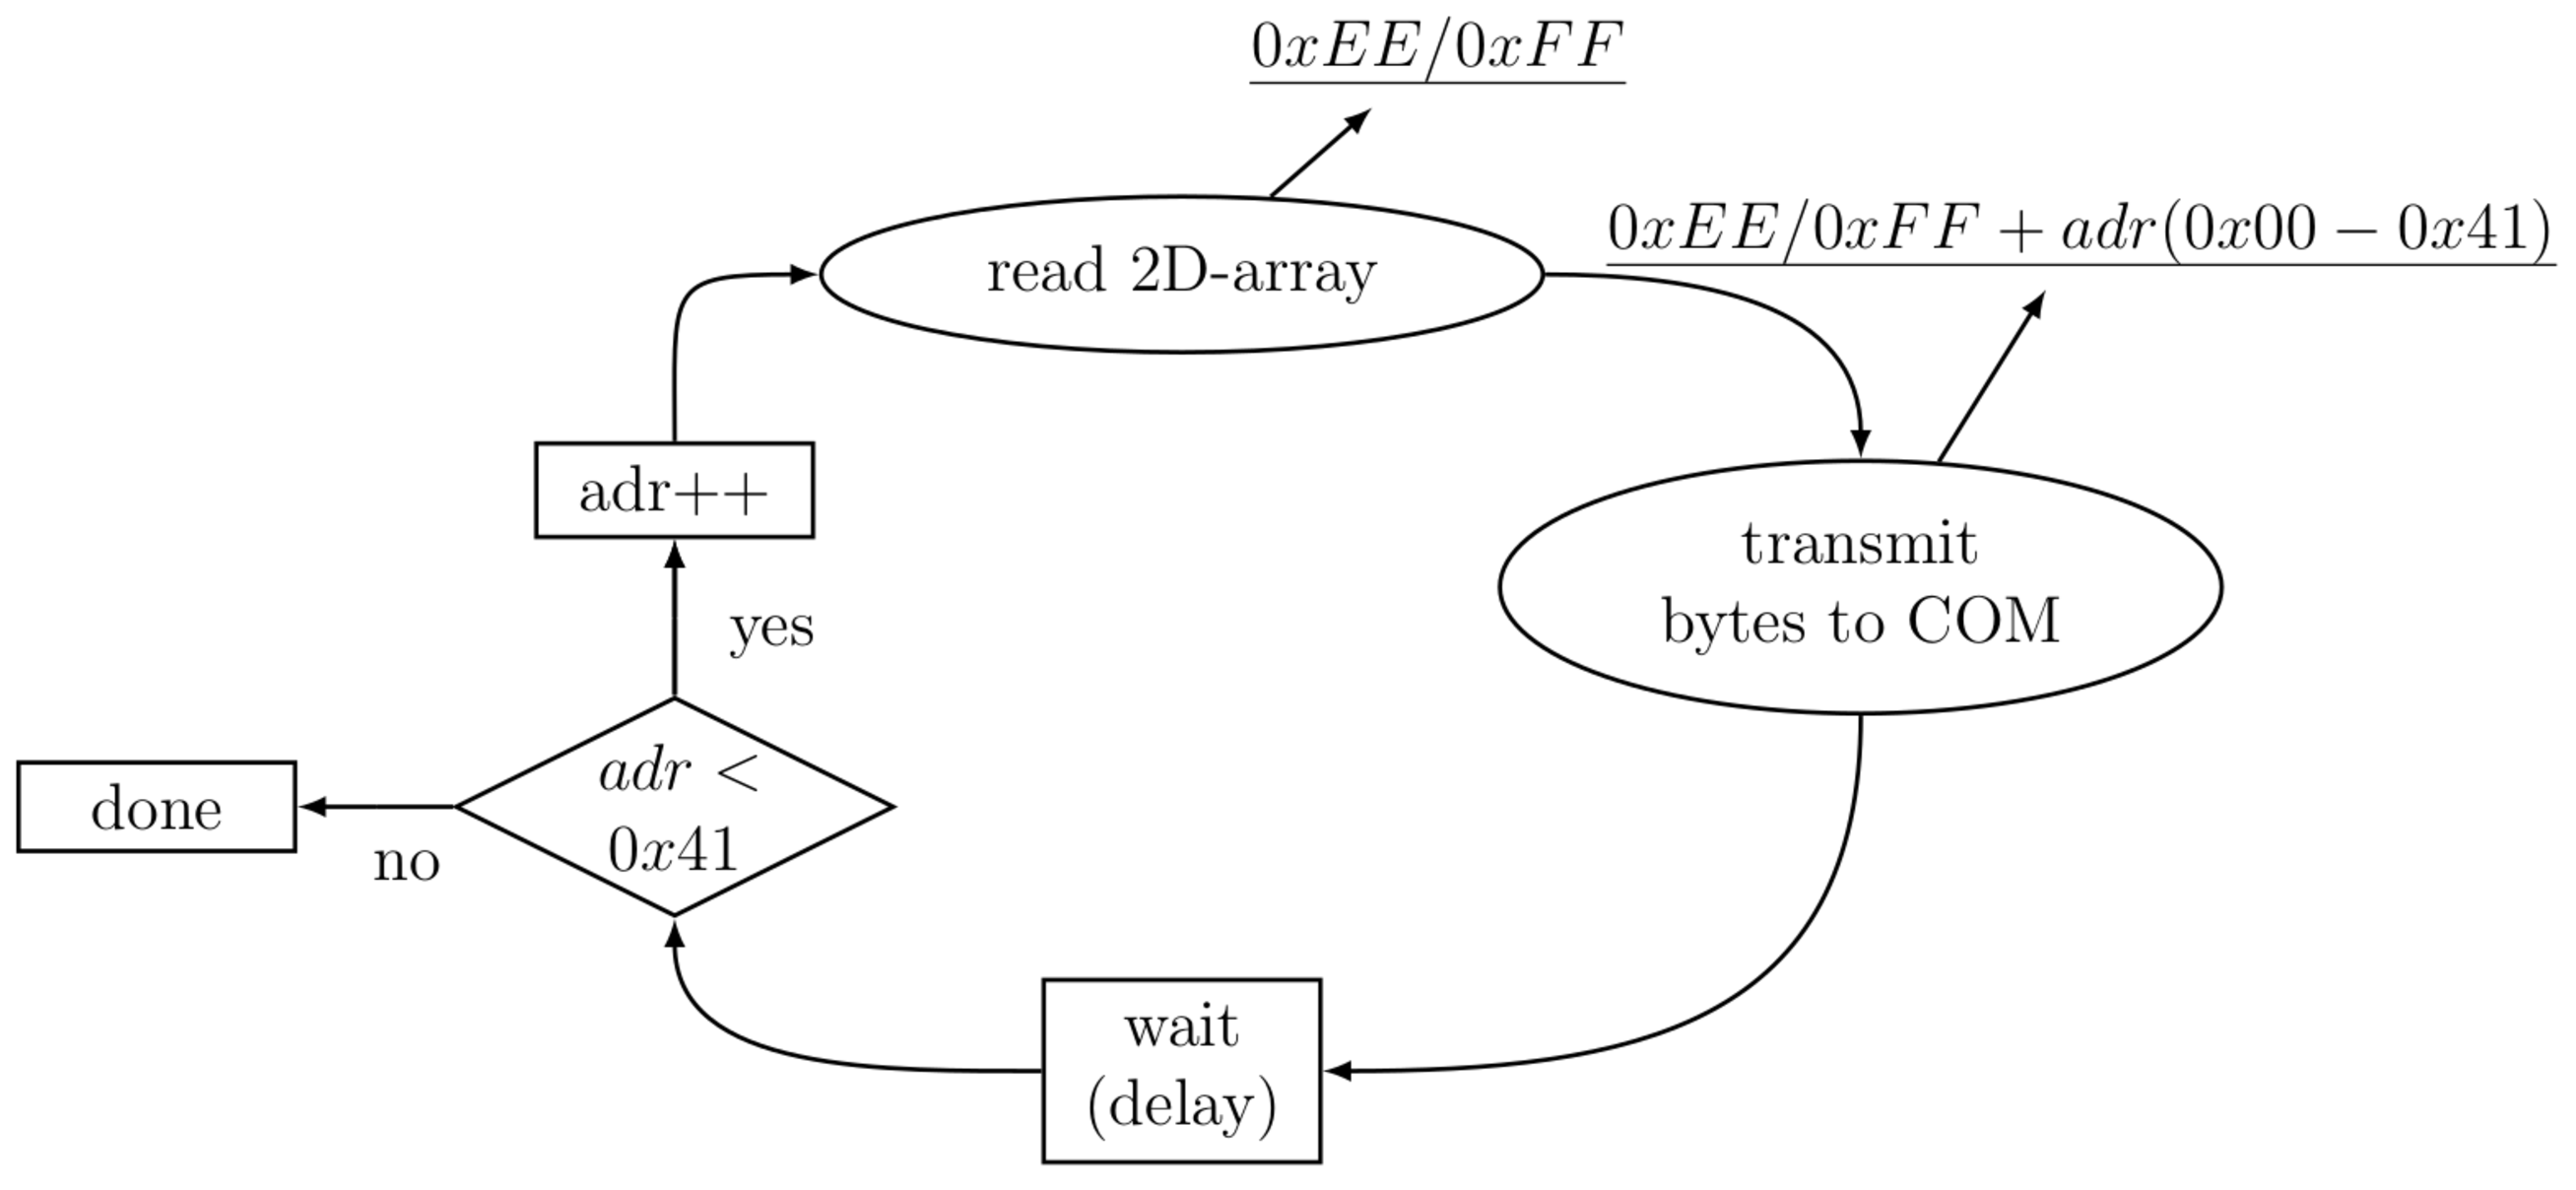
\includegraphics[width=0.8\paperwidth]{../img/tx_cycle.pdf}
% \end{backgroundblock}

% \end{frame}
% %------------------------------------------------

\begin{frame}[b]
\frametitle{User Interface}
\begin{backgroundblock}{0.5cm}{2cm}
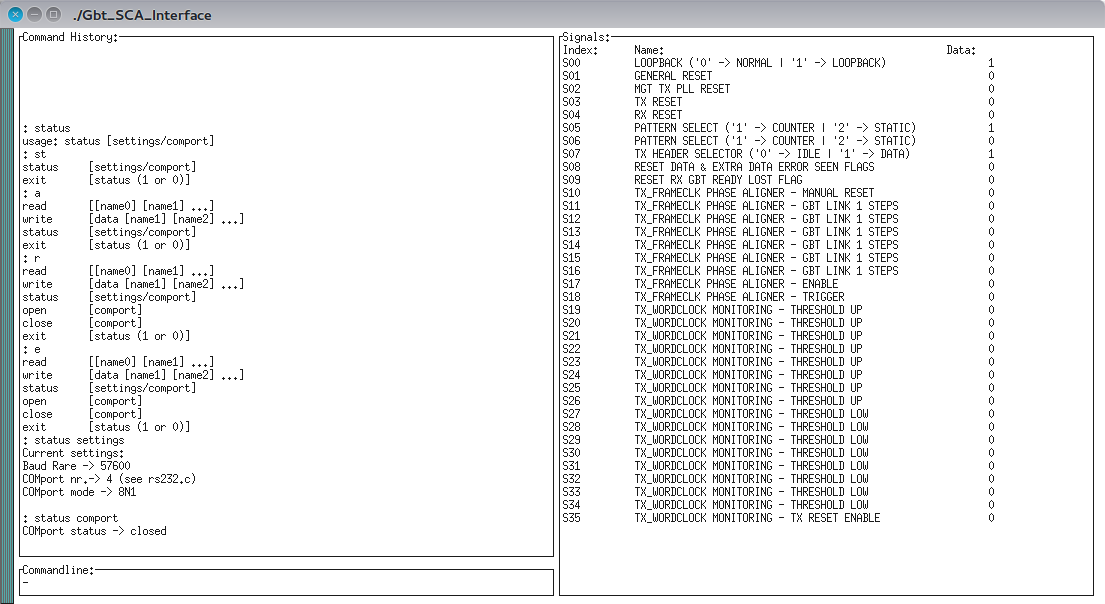
\includegraphics[width=0.9\paperwidth, trim={6mm 0 0 11mm}, clip]{../img/gbt_gui_inv.png}
\end{backgroundblock}

\begin{itemize}
\item Ex.: "write 1 s01 s02 s03"
\end{itemize}

\end{frame}
%------------------------------------------------

%------------------------------------------------
\section{Testing and Verification}
%------------------------------------------------
\subsection{External Loop-back Test}
\subsection{Testing Software and Hardware}
%------------------------------------------------

\begin{frame}[t]
\frametitle{Testing and Verification}

\begin{backgroundblock}{1.5cm}{5.5cm}
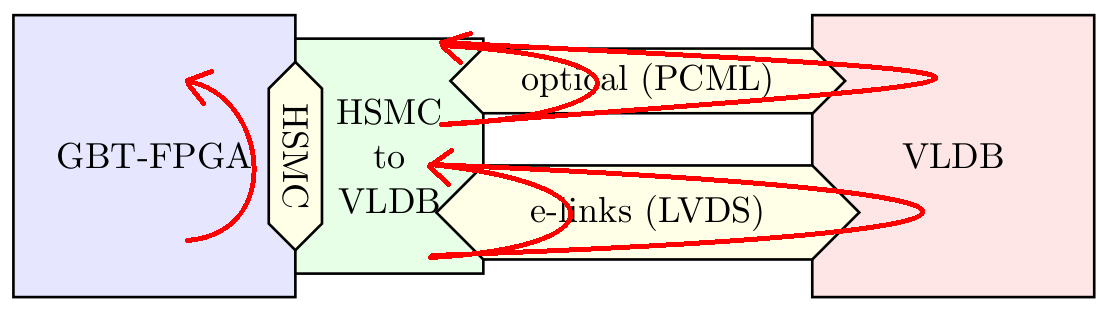
\includegraphics[width=0.8\paperwidth]{../img/loopbackdia.png}
\end{backgroundblock}

\begin{itemize}
\item Internal loopback test using GBT-example
\item External Loopback Tests: HDMI and Optical-Fiber
%\item Hardware Simulation using Testbench in Modelsim
\item Testing Software and Hardware
\end{itemize}

\end{frame}
%------------------------------------------------

\begin{frame}[t]
\frametitle{Test Setup}

\begin{backgroundblock}{0.5cm}{2cm}
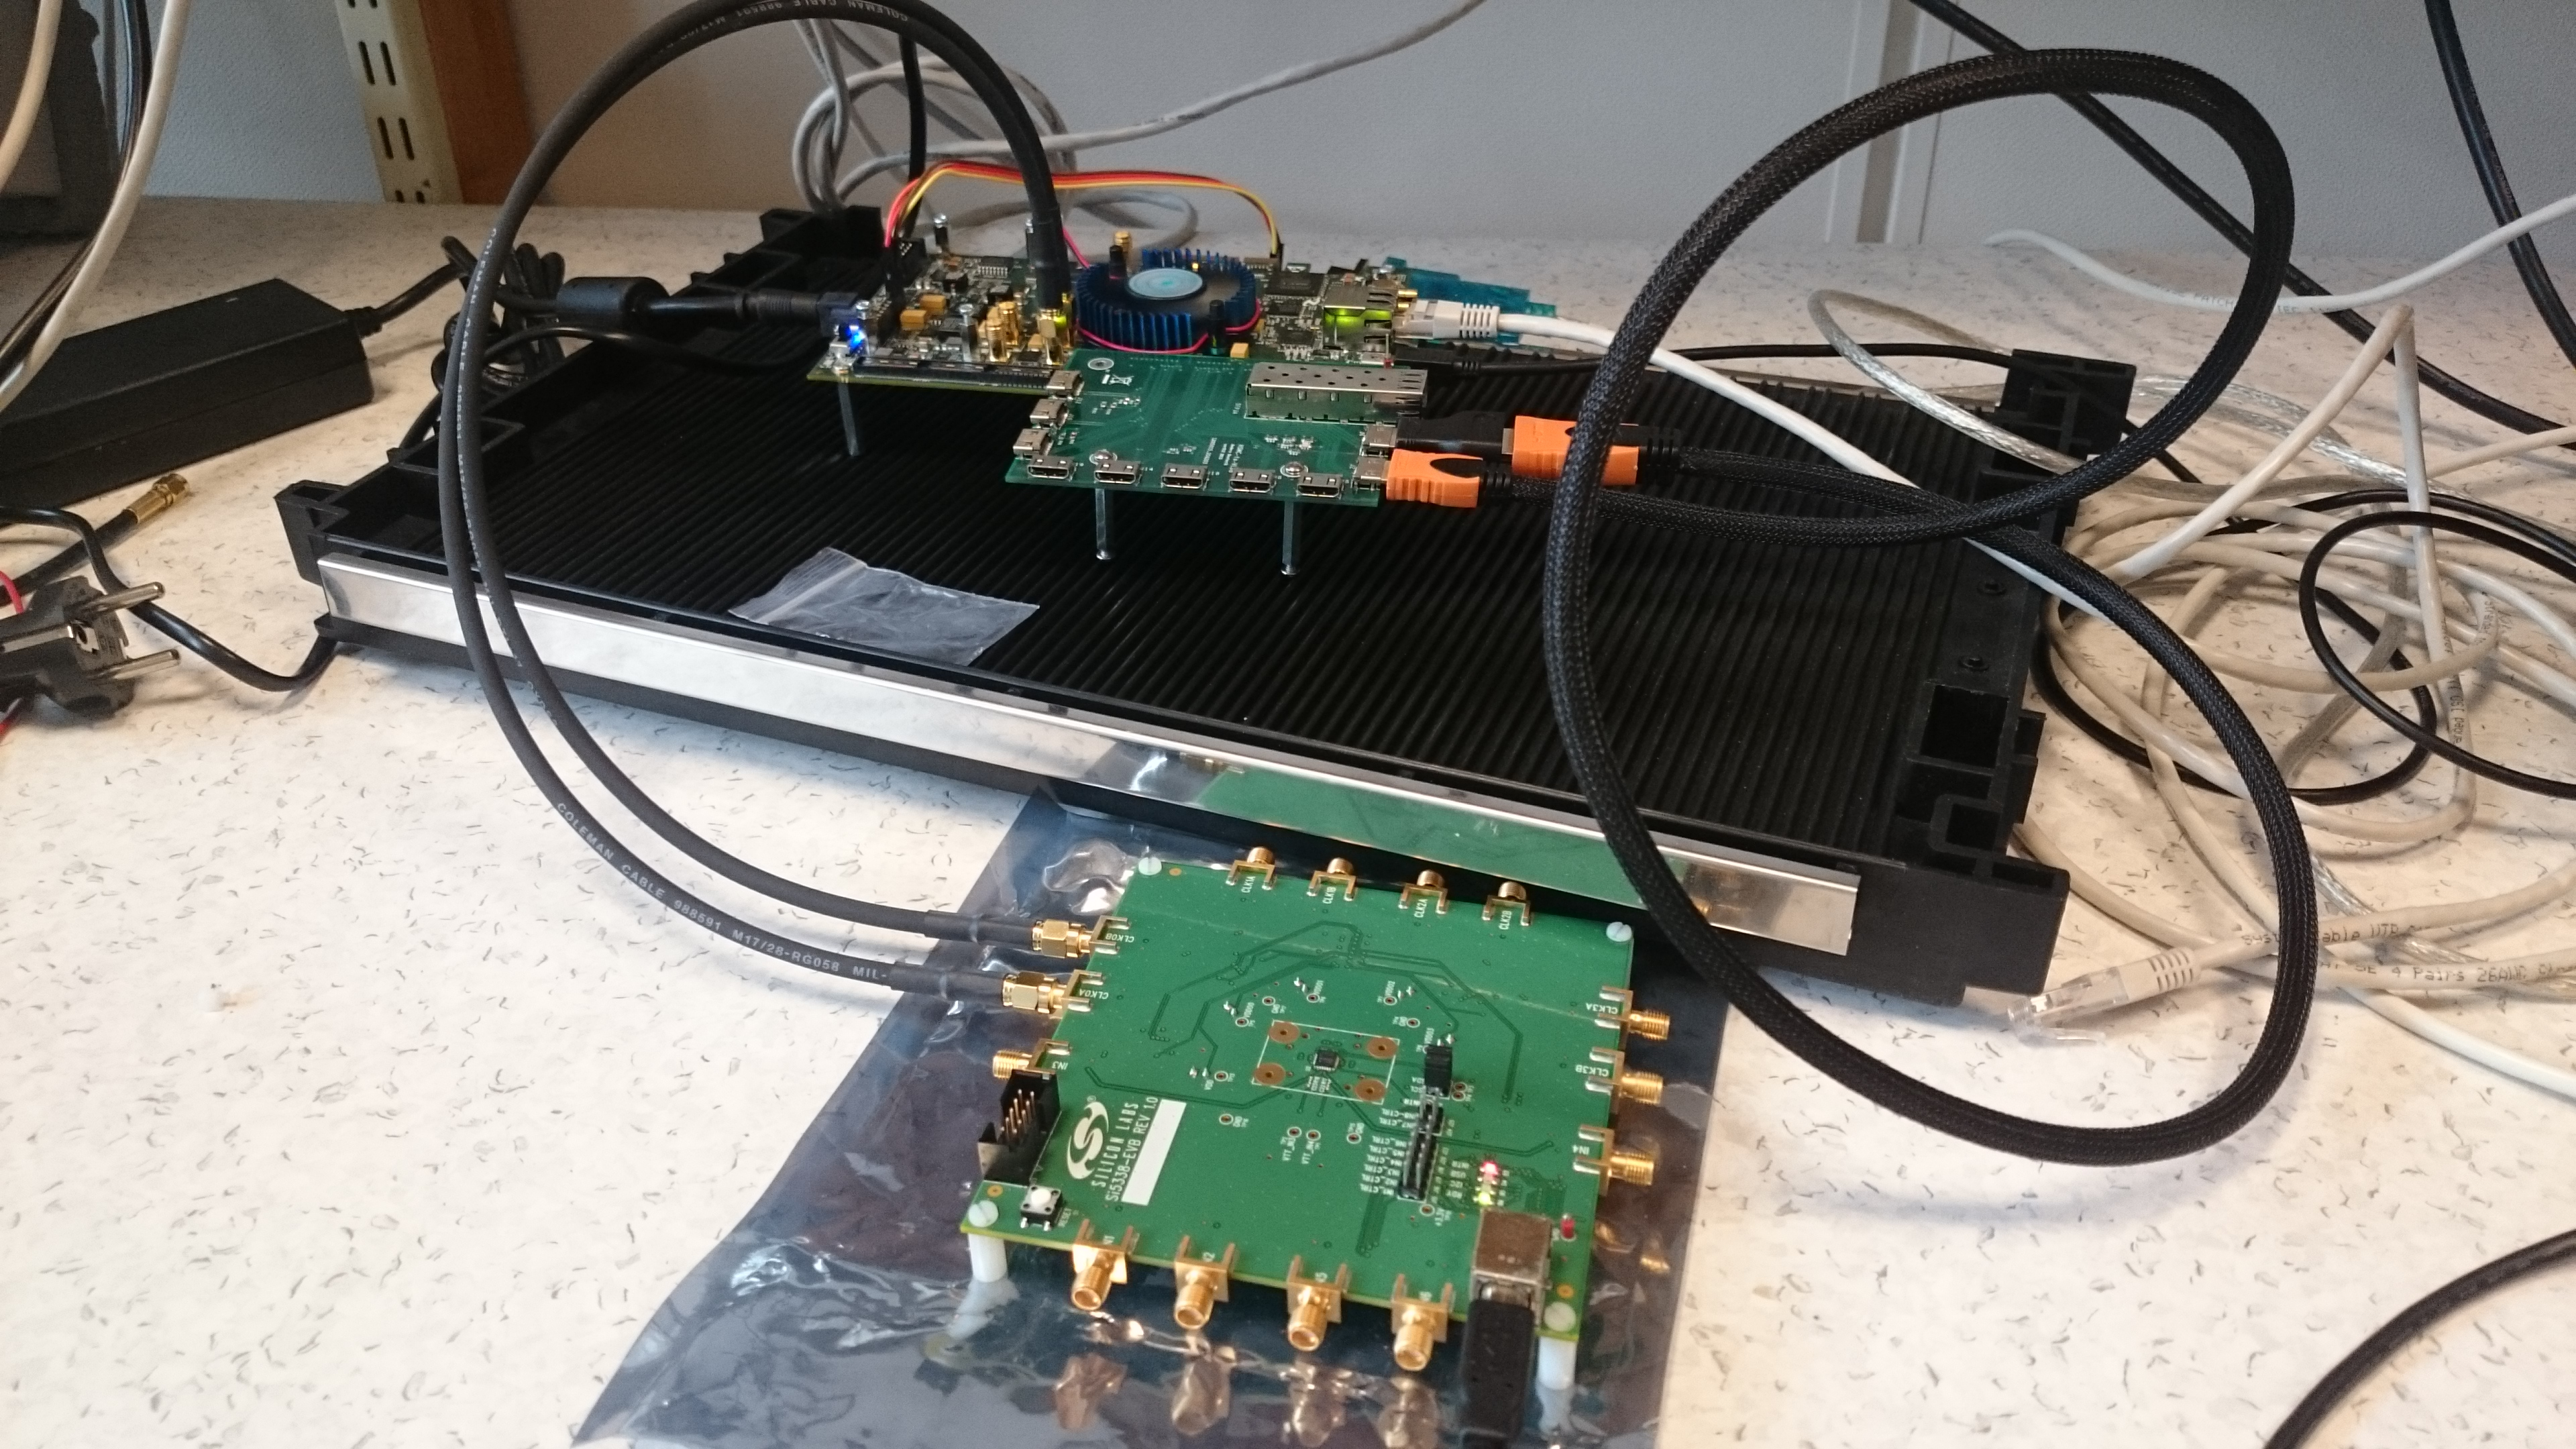
\includegraphics[width=0.9\paperwidth]{../img/setup.JPG}
\end{backgroundblock}

\end{frame}
%------------------------------------------------
\begin{frame}[t]
\frametitle{Test Setup}

\begin{backgroundblock}{0.5cm}{2cm}
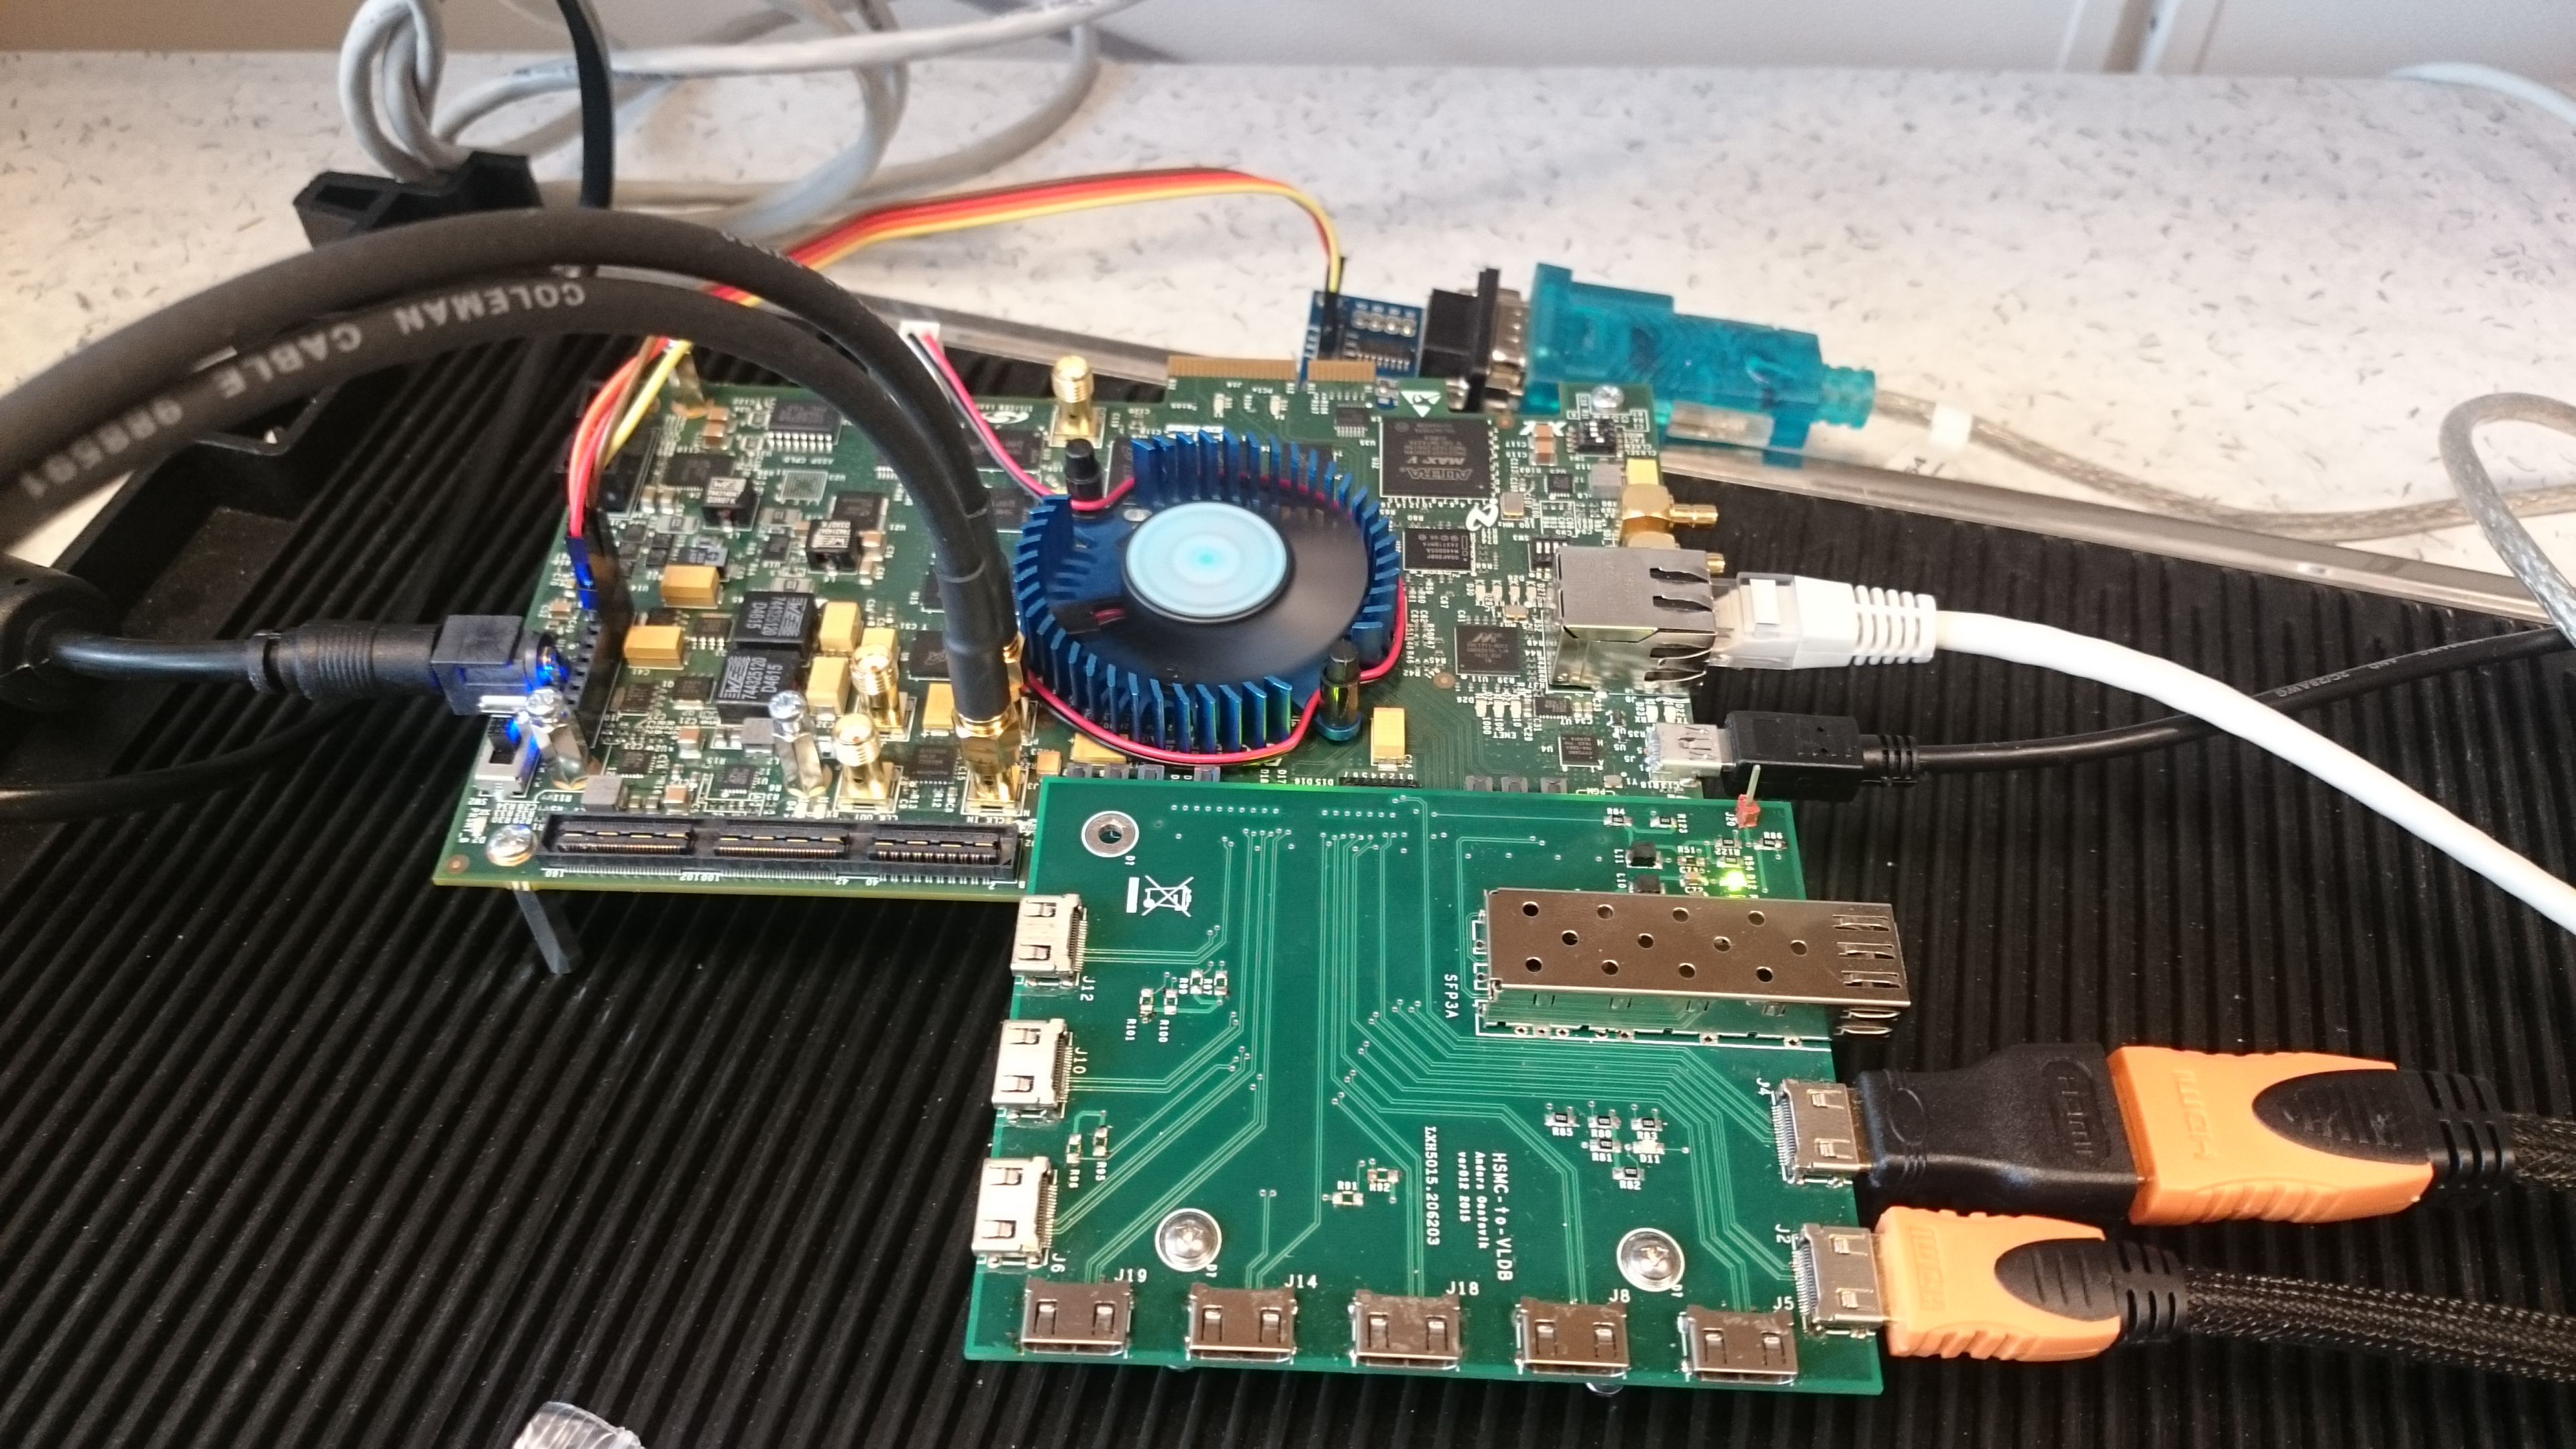
\includegraphics[width=0.9\paperwidth]{../img/setup2.JPG}
\end{backgroundblock}

\end{frame}
%------------------------------------------------

\begin{frame}[t]
\frametitle{External Loop-back Test}

\begin{backgroundblock}{7.5cm}{2.8cm}
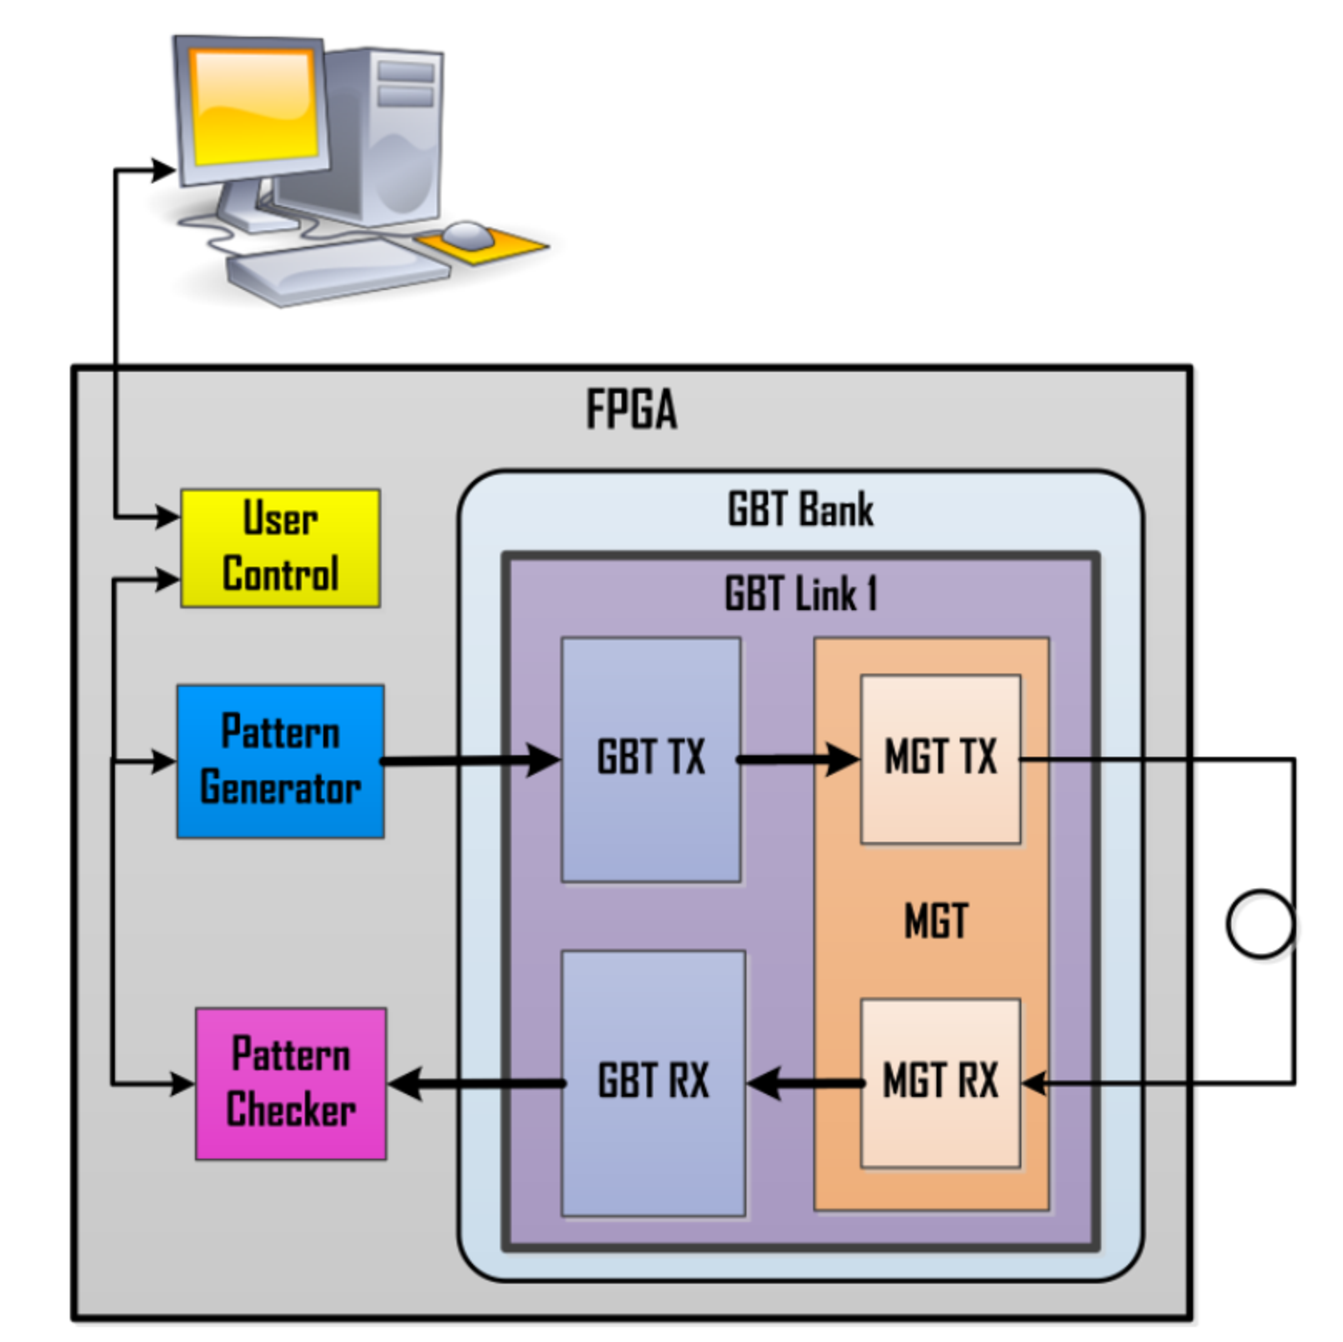
\includegraphics[width=5cm]{../img/gbtex}
\end{backgroundblock}

\begin{backgroundblock}{1.5cm}{5.5cm}
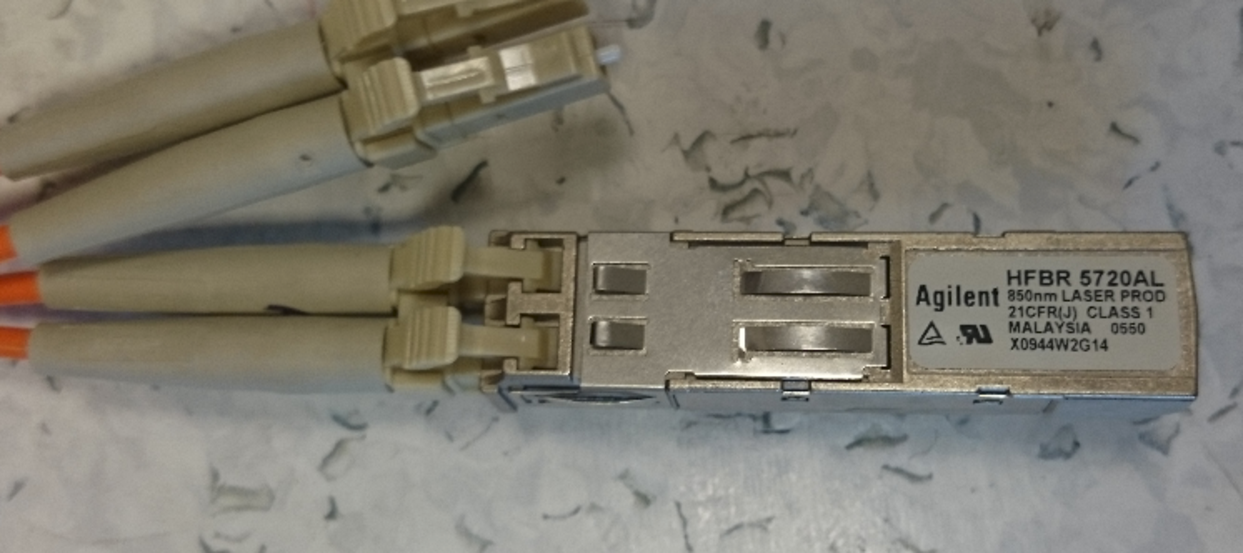
\includegraphics[width=5cm]{../img/laser}
\end{backgroundblock}

\Large Optical Fiber Connector (PCML):\\
\normalsize
\begin{itemize}
\item GBT example Design
\item $4.8~\giga\bit\per\second~counter$
\item Internal-, then external loopback
\item SignalTap II $\rightarrow$ sample TX and RX
\end{itemize}

\end{frame}
%------------------------------------------------

\begin{frame}[t]
\frametitle{External Loop-back Test}

\begin{backgroundblock}{7cm}{5cm}
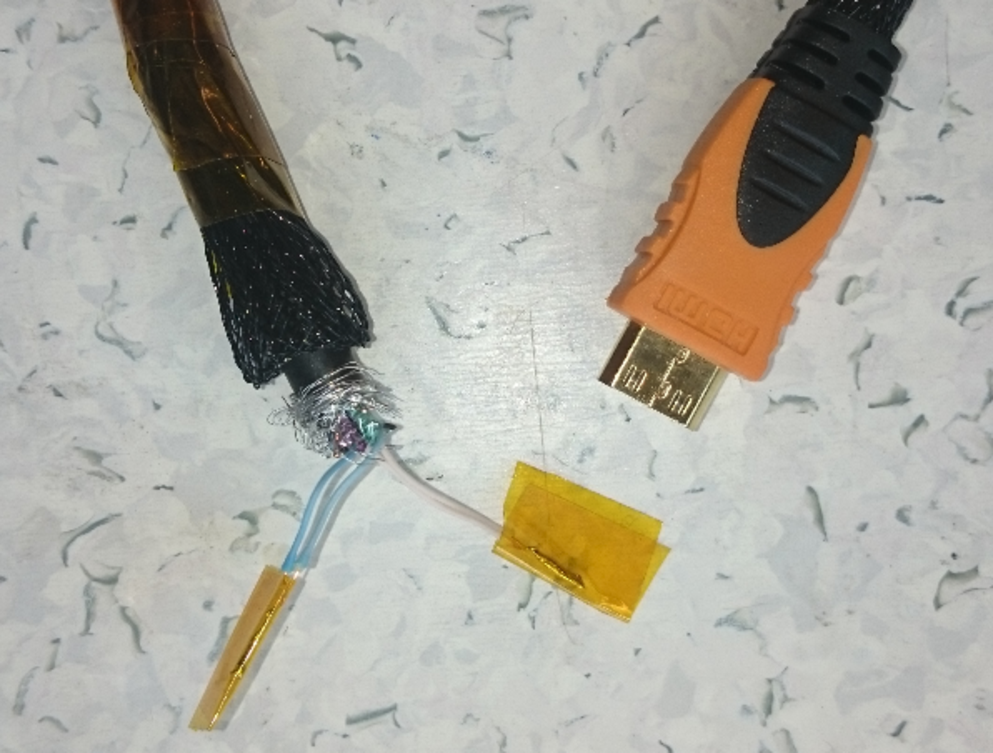
\includegraphics[width=0.4\paperwidth]{../img/hdmilpback}
\end{backgroundblock}

\Large HDMI connectors (LVDS):\\
\normalsize
\begin{itemize}
\item Purpose: Transmission of $320~\mega\bit\per\second$ E-link detector data
\item Test: Loop-back a $300~\mega\hertz$ Pseudo-random counter
\item Measure:
	\begin{itemize}
	\item bit-error count
	\item eye-diagram
	\item crosstalk
	\item reflections
	\end{itemize}
\end{itemize}

\end{frame}
%------------------------------------------------

\begin{frame}[t]
\frametitle{Testing and Verification}

\begin{backgroundblock}{1.5cm}{4cm}
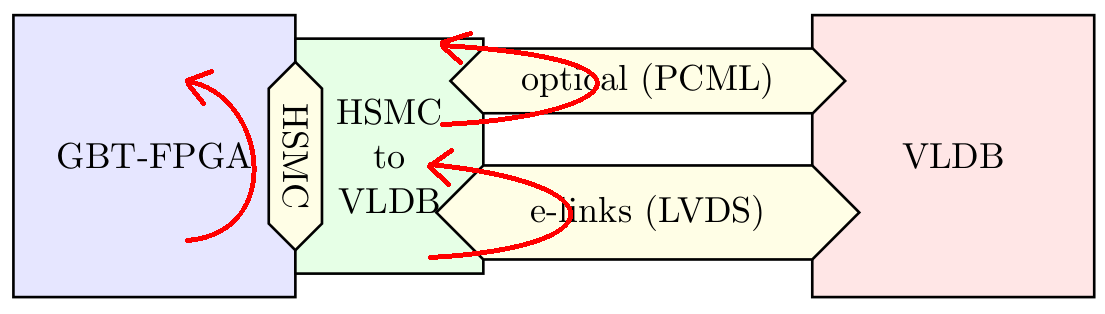
\includegraphics[width=0.8\paperwidth]{../img/loopbackdia2.png}
\end{backgroundblock}

\end{frame}
%------------------------------------------------

\begin{frame}[t]
\frametitle{Testing Software and Hardware}

\begin{itemize}
\item Verified hardware with a testbench $\rightarrow$ Bitvis Utility Library
\item Verified that the software and hardware were communicating
	%\begin{itemize}
	%\item Uart-
	%\end{itemize}
\end{itemize}

\end{frame}
%------------------------------------------------

%------------------------------------------------
\section{Conclusion}
%------------------------------------------------
%\subsection{}
%------------------------------------------------

\begin{frame}[t]
\frametitle{Conclusion}

%\Large PCB:\\
%\normalsize
\begin{itemize}
\item PCB:
	\begin{itemize}
	\item Optical Fiber module \textbf{works} $\rightarrow$ $4.8~\giga\bit\per\second$ external loopback
	\item HDMI LVDS connectors \textbf{needs more testing} $\rightarrow$ eye-diagram, crosstalk, reflections, bit-error count.
	\end{itemize}
\end{itemize}

%\Large Hardware:\\
%\normalsize
\begin{itemize}
\item Hardware:
	\begin{itemize}
	\item UART + Decoder \textbf{works}
	\item Implementation into the GBT Example Design remains
	\end{itemize}
\end{itemize}	

%\Large Software:\\
%\normalsize
\begin{itemize}
\item Software:
	\begin{itemize}
	\item Send/Receive and User Interface modules \textbf{works}
	\item Both needs to be merged
	\end{itemize}
\end{itemize}	

%\vspace{15pt}
%\large A final test of the system as a whole remains

\begin{itemize}
\item Final test of the whole system:
	\begin{itemize}
	\item GBT example + Hardware + Software + PCB-loopback
	\item Test system together with VLDB
	\end{itemize}
\end{itemize}

\end{frame}
%------------------------------------------------

\begin{frame}
\Huge{\centerline{Thank you!}}
\end{frame}

%----------------------------------------------------------------------------------------

\end{document} 